% @author Tobias Wulf
% thesis root document

\documentclass[
  a4paper,            % DIN A4
  DIV=10,             % Schriftgröße und Satzspiegel
  oneside,            % einseitiger Druck
  BCOR=5mm,           % Bindungskorrektur
  parskip=half,       % Halber Abstand zwischen Absätzen
  numbers=noenddot,   % Kein Punkt hinter Kapitelnummern
  bibtotoc,           % Literaturverzeichnis im Inhaltsverzeichnis
  listof=totoc        % Abbildungs- und Tabellenverzeichnis im Inhaltsverzeichnis
]{scrreprt}
\usepackage{./style/thesisstyle}

% redefine reference names for autoref
\addto\extrasngerman{%
	\def\subsubsectionautorefname{Unterabschnitt}%
	\def\paragraphautorefname{Unterabschnitt}%
}
  
\makeglossaries           % create all glossary entries (remember: run makeglossaries manually)
\makeindex
\loadglsentries[main]{./glossaries/glossary}  % load acronym, symbol and glossarie entries
\loadglsentries[\acronymtype]{./glossaries/acronyms}
\loadglsentries[symbols]{./glossaries/symbols}

\addbibresource{./literature/literature.bib}

\sisetup{locale = DE}     % siunitx locale setup
%\DeclareSIUnit \fps{fps}  % a custom unit (usage: \SI{24}{\fps})

% code listings setup
\lstset{style=Matlab-editor,basicstyle=\ttfamily}

\begin{document}
% !TEX root = ../thesis.tex
%
% configurations
%

% text field
%-> replace supervisor names with correct ones
\firstSupervisor{Prof. Dr. Karl-Ragmar Riemschneider}
\secondSupervisor{Prof. Dr. Klaus Jünemann}

% text field
%-> replace title with your thesis title
\thesisTitle{Winkelmessung durch magnetische Sensor-Arrays und Toleranzkompensation mittels Gauß-Prozess}
\thesisTitleEN{Angular Measurement by Magnetic Sensor Arrays and Tolerance Compensation by Gaussian Process}

% text field
%-> replace the key words with your own key words
\keywordsDE{Sensor-Array Simulation, Dipol, Magnetfeld, Kugelmagnetapproximation, TMR, TDK TAS2141, AMR, NXP KMZ60, Toleranzkompensation, Gauß-Prozess, Kovarianzmatrix, Regression, Winkelvorhersage}
\keywordsEN{Sensor Array Simulation, Dipole, Magnetic Field, Sperical Magnet Approximation, TMR, TDK TAS2141, AMR, NXP KMZ60, Tolerance Compensation, Gaussian Process, Covariance Matrix, Regression, Angular Prediction}

% text field
%-> replace the text with a description of the thesis
\abstractDE{\dots}
\abstractEN{\dots}

% text field
%-> replace jon with your name
\thesisAuthor{Tobias Wulf}

% text field
%-> enter the submission date
\submissionDate{TT. Monat Jahr}

% switch - uncomment only one
%-> uncomment NDA or public
%\NDA{yes}
\NDA{no}

% switch - uncomment only one
%-> uncomment cover or cover Corporate Design 2017
%\Cover{CD2017}
%\Cover{CD2017NoLogo}
\Cover{Std2018}

% switch - uncomment only one
%-> uncomment to show list of figures or not
\ListOfFigures{yes}
%\ListOfFigures{no}

% switch - uncomment only one
%-> uncomment to show list of tables or not
\ListOfTables{yes}
%\ListOfTables{no}

% switch - uncomment only one
%-> uncomment to show list of accronyms or not
\ListOfAccronyms{yes}
%\ListOfAccronyms{no}

% switch - uncomment only one
%-> uncomment to show list of symbols or not
\ListOfSymbols{yes}
%\ListOfSymbols{no}

% switch - uncomment only one
%-> uncomment to show list of glossary entries or not
\Glossary{yes}
%\Glossary{no}

% switch - uncomment only one
%-> uncomment the study course you are in
%\studycourse{ITS}
%\studycourse{TI}
%\studycourse{AI}
%\studycourse{WI}
\studycourse{EI}
%\studycourse{REE}
%\studycourse{BMT}
%\studycourse{MAI}
%\studycourse{MIK}
%\studycourse{MA}
    % load all settings

\hyphenation{Ba-che-lor-the-sis Mas-ter-the-sis}

% Cover page here, no page number
\ICoverPage

% PDF Metadata
% !TEX root = ../thesis.tex
%
% PDF Metadata integration
% @author Thomas Lehmann
%

% PDF Metadata
\hypersetup{
pdftitle={\IthesisTitle},
pdfauthor={\IthesisAuthor},
pdfkeywords={\IkeyWordsEN}
}

% Titlepage is page one even if the number is not shown.
\pagenumbering{roman}
% Title page here
% !TEX root = ../thesis.tex
%
% title page
% @author Thomas Lehmann
% Hints for title page and page numbering: https://en.wikipedia.org/wiki/Title_page
%
\title{\IthesisTitle}   % set latex default title to be used by hyperref in pdf
\author{\IthesisAuthor} % set latex default author to be used by hyperref in pdf

\newpage
\thispagestyle{empty}
{\fontfamily{phv}\selectfont
  \hfuzz=20pt       % suppress warnings due to extenstion onto page margins

  % Author of thesis
  \vspace*{1cm}
  \begin{minipage}[b]{\textwidth}
    \fontsize{14pt}{20pt}
    \selectfont
    \begin{center}
      \IthesisAuthor
    \end{center}
  \end{minipage}

  % Title of thesis
  \vspace{1.5cm}
  \begin{minipage}[b][0cm][t]{\textwidth}
    \fontsize{18pt}{20pt}
    \selectfont
    \begin{center}
      \IthesisTitle
    \end{center}
  \end{minipage}

  % Important information
  \begin{textblock*}{\textwidth}(40mm,210mm)
    \begin{minipage}[b]{\textwidth}
      \hbadness=10001    % suppress underfull warning due to short text
      \fontfamily{cmr}\selectfont
      \fontsize{12pt}{14pt}
      \selectfont
      \IthesisKindDE ~eingereicht im Rahmen der \IthesisExaminationDE \\
      im Studiengang \textit{\IstudyCourseName} \\
      am \IthesisDepartmentFull \\
      der Fakultät Technik und Informatik\\
      der Hochschule für Angewandte Wissenschaften Hamburg\\

      Betreuender Prüfer: \IfirstSv \\
      Zweitgutachter: \IsecondSv \\

      Eingereicht am: \ISubDate \\
    \end{minipage}
  \end{textblock*}
}


% Abstract page here
% !TEX root = ../thesis.tex
%
% abstract page
% @author Thomas Lehmann
%
\newpage
\thispagestyle{plain}
\clearpage
\hfuzz=12pt       % suppress warnings due to extenstion onto page margins

\textbf{\IthesisAuthor}

\vspace{0.3cm}
\textbf{Thema der Arbeit}

\IthesisTitle

\vspace{0.3cm}
\textbf{Stichworte}

\IkeyWordsDE

\vspace{0.3cm}
\textbf{Kurzzusammenfassung}

\begin{minipage}{\textwidth}
\IabstractDE
\end{minipage}

\vspace{1.0cm}
\textbf{\IthesisAuthor}

\vspace{0.3cm}
\textbf{Title of Thesis}

\IthesisTitleEN

\vspace{0.3cm}
\textbf{Keywords}

\begin{minipage}{\textwidth}
\IkeyWordsEN
\end{minipage}

\vspace{0.3cm}
\textbf{Abstract}

\IabstractEN


%adjust spacing in table of contents
\setlength{\cftsubsubsecnumwidth}{4.8em}
\setlength{\cftparanumwidth}{5.8em}

% Table of contents here
\tableofcontents

% Uncomment if list of source code is needed (rarely).
%\lstlistoflistings  % requires package listings, needs to uncommenting of usepackage

% path to the chapters folder is set to find the images used there
\graphicspath{%
	 {./chapters/images}%
	 {./chapters/images/1-Motivation}%
	 {./chapters/images/2-Grundlagen}%
	 {./chapters/images/3-SW-E-OExp}%
	 {./appendix/images}%
	 {./appendix/images/3-TDK}%
	 {./appendix/images/4-KMZ60}%
	 {./appendix/images/5-Sensor-Array-Simulation}%
	 {./appendix/images/8-Ergebnisse-Experimente}%
}

% Chapters
\clearpage
\pagenumbering{arabic}
% Add additional chapters here
% !TEX root = ../thesis.tex
% introduction
% @author Tobias Wulf
%

\chapter{Motivation 0.0.1 17.02.2021}

Neuentwicklungen in der Halbleitertechnik, auf Basis des \gls{gl:tmr}s, ermöglichen den Aufbau komplexerer Sensorstrukturen \cite{Schuethe2019}. Die \gls{gl:ags} an der \gls{gl:haw} erforscht moderne Ansätze der Signalverarbeitung für neugewonnene Sensorstrukturen, verwirklicht als magnetische Sensor-Arrays. Durch den Aufbau von Sensoren als Arrays, bieten sich Möglichkeiten zur Nutzung von Algorithmen und Regressionsverfahren an, die eine Kompensation und Detektion von mechanische Toleranzen zulassen \cite{Schuethe2020}.
\newline
Das Verarbeiten einer Vielzahl an Messwerten, bedingt durch Sensor-Array-Strukturen, ist hierbei eine der Herausforderungen die es zu bewältigen gilt. Mit Hilfe moderner Algorithmen, die Ansätze des maschinellen Lernens beinhalten, ergeben sich weitere Problemstellungen in Bezug auf Modellabbildung- und Optimierung.
Das übergeordnete Ziel bei der Lösung und Bewältigungen der einzelnen Etappen ist die Verbesserung der Messgenauigkeit, indem individuelle Abweichungen des Sensors einem geeigneten Modell antrainiert und Modellparameter optimiert werden. Moderne Regressionsverfahren liefern dabei statistische Ansätze um geeignete Qualitätskriterien zu bilden und somit trainierte Modelle und ihre Messwertgenauigkeit zu bewerten.

% !TEX root = ../thesis.tex
% goals
% @author Tobias Wulf
%

\section{Zielstellung 0.0.1 14.01.2021}

% !TEX root = ../thesis.tex
% basics
% @author Tobias Wulf
%

\chapter{Grundlagen 0.0.2 19.02.2021}\label{ch:grundlagen}
	\begin{itemize}
		\item Einleitung Aufgabenfeld
		\item Einheitskreis
		\item Bezug zur Drehwinkelerfassung und Sensorapplikation
	\end{itemize}

\section{Magnetische Sensorentypen und mechatronische Anwendung}\label{sec:magnetische-sensorentypen}
	\begin{itemize}
		\item Die Technologie mit der ein Sensorkopf realisiert ist, klassifiziert in der Regel die Sensorbezeichnung. Anhänge in der Bezeichnung wie AMR oder TMR, geben somit Auskunft darüber welche Technologie für die Realisierung des Sensorkopfes die Grundlage bildet.
		\item Anwendungsfall Winkelmessung
		\item Aufbau Sensorbrücke TMR (Umriss aus Datenblatt)
		\item Ausblick TMR Drehzahlmessung und Strommessung
	\end{itemize}

\section{Kennfeldmethode zur Charakterisierung von Sensoren}\label{sec:kennfeldmethode-zur-charakterisierung}
	\begin{itemize}
		\item Überleitung von Sensorbrückenschaltung
		\item Messprinzip für das Erstellen der Sensorbrücken-Kennfelder
		\item Festlegung von Arbeitsbereich (Plateau TMR), Sättigung (KMZ60)
		\item Dimensionierung des Stimulus, Dipole Anregung
	\end{itemize}

\section{Prinzip des Sensor-Arrays}\label{sec:prinzip-des-sensor-arrays}
	\begin{itemize}
		\item geometrischer Aufbau
		\item Brückenausgangsspannungen
		\item Resultierende Array-Datenformate und Darstellung der Sinoiden
	\end{itemize}

\section{Sensor-Array-Simulation über Dipol-Feldgleichung}\label{sec:sensor-array-simulation-dipol-feldgleichung}
	\begin{itemize}
		\item Erzeugen des Meshgrids
		\item Normieren des Magnetfeldes
		\item Erzeugen von Rotationsmomenten (inkl. Verkippung)
		\item Referenzierung zu Kennfeldern und Gewinnung der Brückenspannungen (interp2 nearest neighbor)
	\end{itemize}

\section{Gauß-Prozesse für Regressionsverfahren}\label{sec:gauss-prozesse-regressionsverfahren}
	\begin{itemize}
		\item Erläuterung des Regressionsverfahren im allg.
		\item Bedeutung und Kriterien der Kovarianzfunktion, Spiegel der Applikation
		\item Herleitung der Quadratischen Frobenius Kovarianzfunktion mit Bezug zum Einheitskreis
		\item Möglichkeiten zur Mittelwertschätzung und -Korrektur
		\item Optimierungskriterien in der Trainingsphase
		\item Qualitätskriterien in der Arbeitsphase
	\end{itemize}
% !TEX root = ../thesis.tex
% developping software for optimization experiments
% @author Tobias Wulf
%

\chapter{Software-Entwicklung für Optimierungsexperimente 0.0.4 25.04.2021}\label{ch:sw-entwicklung-f-opt-exp}


Die Software-Entwicklung erfolgt unter dem Gesichtspunkt zur Durchführung von Versuchsreihen. Ziel ist dabei die Parameterfindung zur Modelloptimierung für die Winkelauswertung. Durchzuführende Simulationen und  Erprobungsexperimente basieren teilweise auf Zwischenergebnissen, die strukturiert im Software-Projektverzeichnis zwischengespeichert sind, siehe \autoref{mcode:project-structure}. Für die Auswertung der Simulationen sind unterstützende Grafiken angefertigt worden. Diese sind als Funktionen im \autoref{mcode:plotfunctions} und in den ausführbaren Skripten im \autoref{mcode:executable-scripts} enthalten. Das Kapitel dient zur näheren Erläuterung des modularen Software-Aufbaus und der zur Verfügung stehenden Simulationsprozesse. Die Entwicklungs-Roadmap der Simulations-Software ist mit Aufführung der einzelnen Beiträge in \autoref{mcode:gaussianprocessdipolesimulation} einzusehen.


% !TEX root = ../thesis.tex
% build and function
% @author Tobias Wulf
%


\section{Aufbau und Funktion}\label{sec:aufbau-und-funktion}


Als erster Schritt der hier stattfindenden Entwicklungsarbeiten wird ein Konzept aufgestellt, dass den erheblichen Simulationsaufwand praktisch benutzbar macht. Dafür sind die Simulationsbestandteile nach Aufgabenbereich und Charakter in \autoref{fig:software-gesamtansicht} zugeteilt. Die Implementierung erfolgt in zwei eigenständigen Simulationen. Für das Sensor-Array mittels Dipol-Feldgleichung in \autoref{ch:sensor-array-sim-imp} und für die ASIC Simulation mit Gauß'scher Prozess-Regression in \autoref{ch:gpr-imp}. Zur Klassifizierung der Simulationen dienen hierbei Datendirektion und Datenbeschaffenheit in den einzelnen Simulationsabschnitten. Die Kopplung und Steuerung beider Simulationsabschnitte erfolgt über Datensätze. Die Datensatzbeschreibung und ihre Nutzung ist im \autoref{mcode:datasets} nachzulesen. 


\clearpage


\begin{figure}[htp]
	\centering
	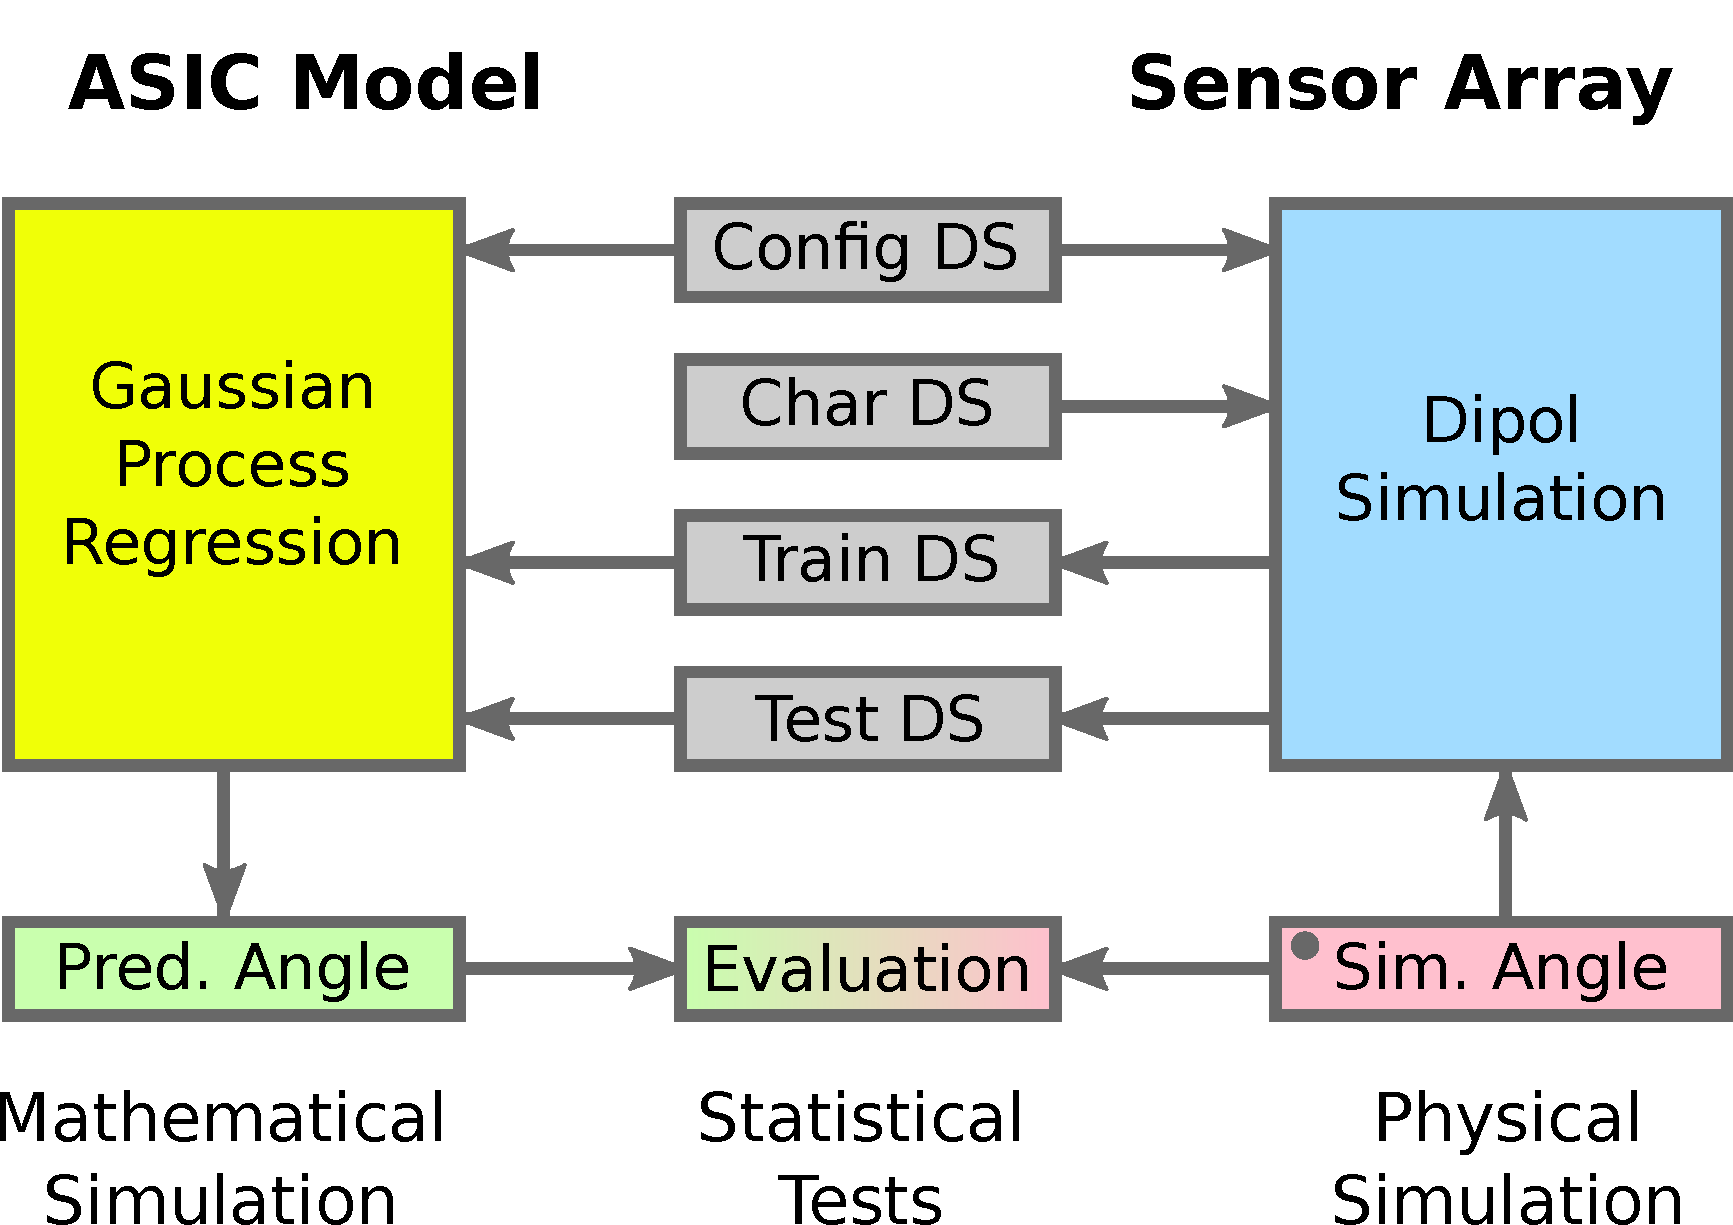
\includegraphics[width=0.7\linewidth]{chapters/images/3-SW-E-OExp/Software-Gesamtansicht}
	\caption[Simulationsaufbau im Überblick]{Simulationsaufbau im Überblick. Konzeptionelle Aufteilung der Simulationen für Sensor-Array und ASIC nach Simulationscharakter. Simulative Kopplung erfolgt, durch prozessierte Datensätze (DS). Eine statistische Auswertung bezieht sich auf angefahrene Simulationswinkel. Der Punkt kennzeichnet die Simulationswinkeleingabe und markiert den gedanklichen Startpunkt des Gesamtkonzepts.}
	\label{fig:software-gesamtansicht}
\end{figure}


Im ersten Simulationsschritt (Sensor-Array) werden Trainings- und Testdatensätze erzeugt. Die Datengenerierung in der Simulation basiert auf Charakterisierungsdatensätze. Diese stellen Technologieeigenschaften und Verhalten für die Simulation bereit, siehe \autoref{ch:tdk-datensatz}. Zur Datengenerierung sind physikalische Gleichungen aus \autoref{sec:sensor-array-simulation-dipol-feldgleichung} genutzt. Als zweiter Simulationsschritt (ASIC-Modell) folgt die Analyse der generierten Daten aus Schritt eins. Zur Analyse wird ein mathematisches Regressionsverfahren verwendet, siehe \autoref{sec:gauss-prozesse-regressionsverfahren}. Das Regressionsverfahren gewichtet Daten und macht entsprechende Vorhersagen gemäß eingestellter Regressionsziele und gewichteten Referenzdaten \autoref{ch:gpr-imp}. Das sind rein mathematische Vorhersagen für vorgegebene Funktionen. Ein physikalischer Gesamtbezug ist durch eine verbundene Auswertung beider Simulationsabschnitte herzustellen. Die Simulationssteuerung ist über einen gemeinsamen Konfigurationsdatensatz umgesetzt, siehe \autoref{tab:sensor-array-sim-params} und \autoref{tab:gpr-sim-params}. Die jeweiligen Parametergruppen sind entsprechend ihrer Zugehörigkeit partiell in den Simulationsbetrieb eingebunden. Der Konfigurationsdatensatz kann je nach Bedarf erzeugt und manipuliert werden. Zur Konfigurationsgenerierung ist das Skript aus \autoref{mcode:generateconfigmat} zu verwenden.


\clearpage


Die Zweischritt-Lösung bietet den Vorteil, dass zuerst verschiedenste Trainings- und Testdatensätze generiert werden können. Nachfolgende und voneinander variierende Simulationen basieren hierbei auf gleichen Datensätzen. Sie sind damit vergleichbar für weitere Auswertungen, Diagnosen oder Optimierungen. Ein empfohlener Arbeitsablauf ist in \autoref{mcode:simulation-workflow} festgehalten.
\newline
Zur Gestaltung der Simulations-Software ist ein modularer Ansatz nach \autoref{fig:blockschemasoftware} verfolgt worden. Das modulare Konzept erhöht die Wiederverwendbarkeit des Quellcodes. Es ermöglicht einzelne Quellcodebestandteile miteinander zu kombinieren. Die Einbindung und Ausführung der Quellcodemodule aus \autoref{mcode:source-code} erfolgt in Skripten des \autoref{mcode:executable-scripts}. Die Software ist als Projekt in der Multi-Paradigmen-Programmiersprache Matlab umgesetzt, siehe \autoref{ch:genutzte-sw}. Konzeptrichtlinien sind im \autoref{mcode:workflows} festgehalten. Zusätzliche Anweisungen zur Arbeitsweise, Projektpflege, Dokumentation und Vorlagen für Skripte und Funktionen sind beigefügt. Alle Entwicklungsschritte sind mittels Git-Versionsverwaltung kommentiert und nachvollziehbar dokumentiert. Jede Quellcode- und Skript-Datei ist nach festgelegten Konventionen geschrieben worden \cite{Johnson2014}. Es ermöglicht eine automatisierte Dokumentation des gesamten Software-Projekts in \autoref{ch:sw-doku}. Erzeugt ist diese mit Skripten aus \autoref{mcode:publishprojectfilestohtml} und \autoref{mcode:exportpublishedtopdf}.


\vspace{3mm}
\begin{figure}[bph]
	\centering
	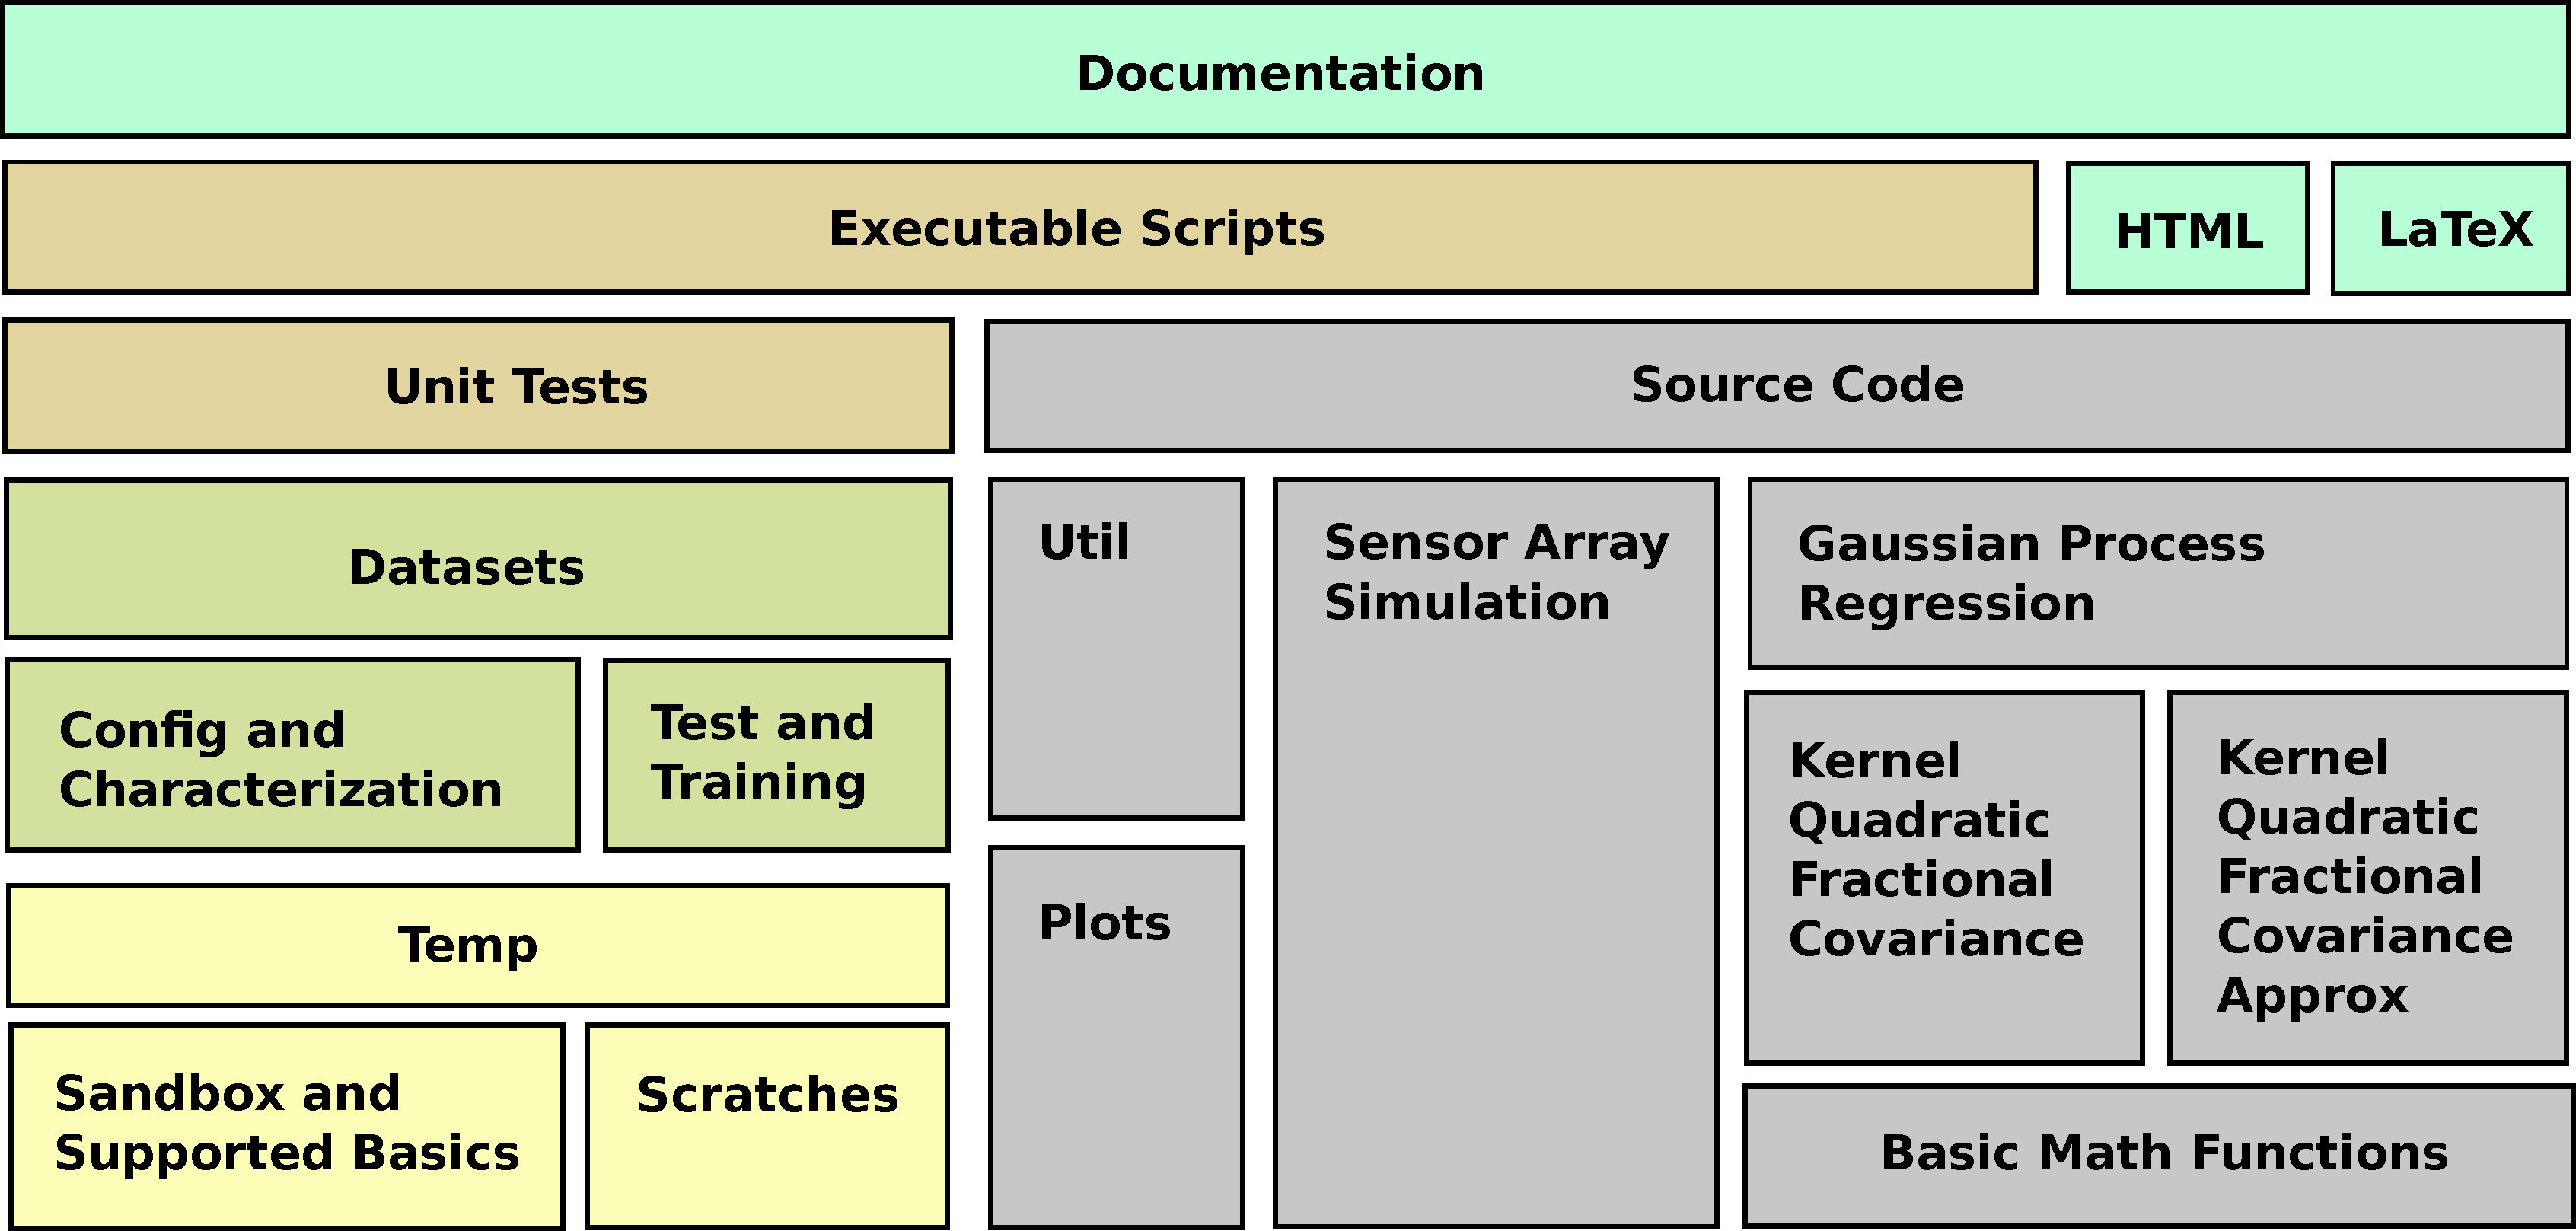
\includegraphics[width=\linewidth]{chapters/images/3-SW-E-OExp/Blockschema_Software}
	\caption[Blockschema Simulations-Software]{Blockschema Simulations-Software. Modulare Software-Gestaltung. Kernbestandteil ist funktionaler Quellcode. Quellcodemodule sind mit Datensätzen nach Bedarf in Skripten zu laden und ausführbar. Software-Dokumentation steht in HTML und LaTeX bereit. Als HTML ist diese in Matlab integriert. Entwurfsarbeiten sind nicht Bestandteil der Dokumentation, aber im Projektverzeichnis vorliegend.}
	\label{fig:blockschemasoftware}
\end{figure}


\clearpage

% !TEX root = ../thesis.tex
% simulation processes and execution
% @author Tobias Wulf
%

\section{Simulationsprozesse und Ausführung}\label{sec:sim-pro}


\subsection{Sensor-Array-Simulation}\label{sub:sensor-array-pro}


\begin{figure}[tbph]
	\centering
	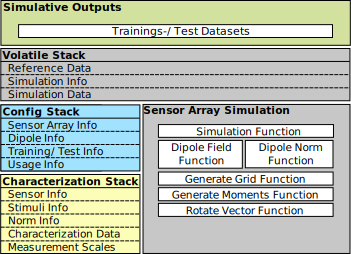
\includegraphics[width=0.7\linewidth]{chapters/images/3-SW-E-OExp/Blockschema_Sensor-Array}
	\caption[Blockschema Einbindung der Sensor-Array-Simulation]{Blockschema Einbindung der Sensor-Array-Simulation}
	\label{fig:blockschemasensor-array}
\end{figure}


\clearpage


\begin{figure}[tbph]
	\centering
	\includegraphics[width=\linewidth]{chapters/images/3-SW-E-OExp/Sensor-Array-Simulation}
	\caption[Sensor-Array-Simulation Prozessansicht]{Sensor-Array-Simulation Prozessansicht}
	\label{fig:sensor-array-simulation}
\end{figure}


\clearpage


\subsection{Gauß-Prozess-Regression}\label{sub:gpr-pro}


\paragraph{Trainingsphase}\label{par:gpr-training-pro}$~$\\


\begin{figure}[tbph]
	\centering
	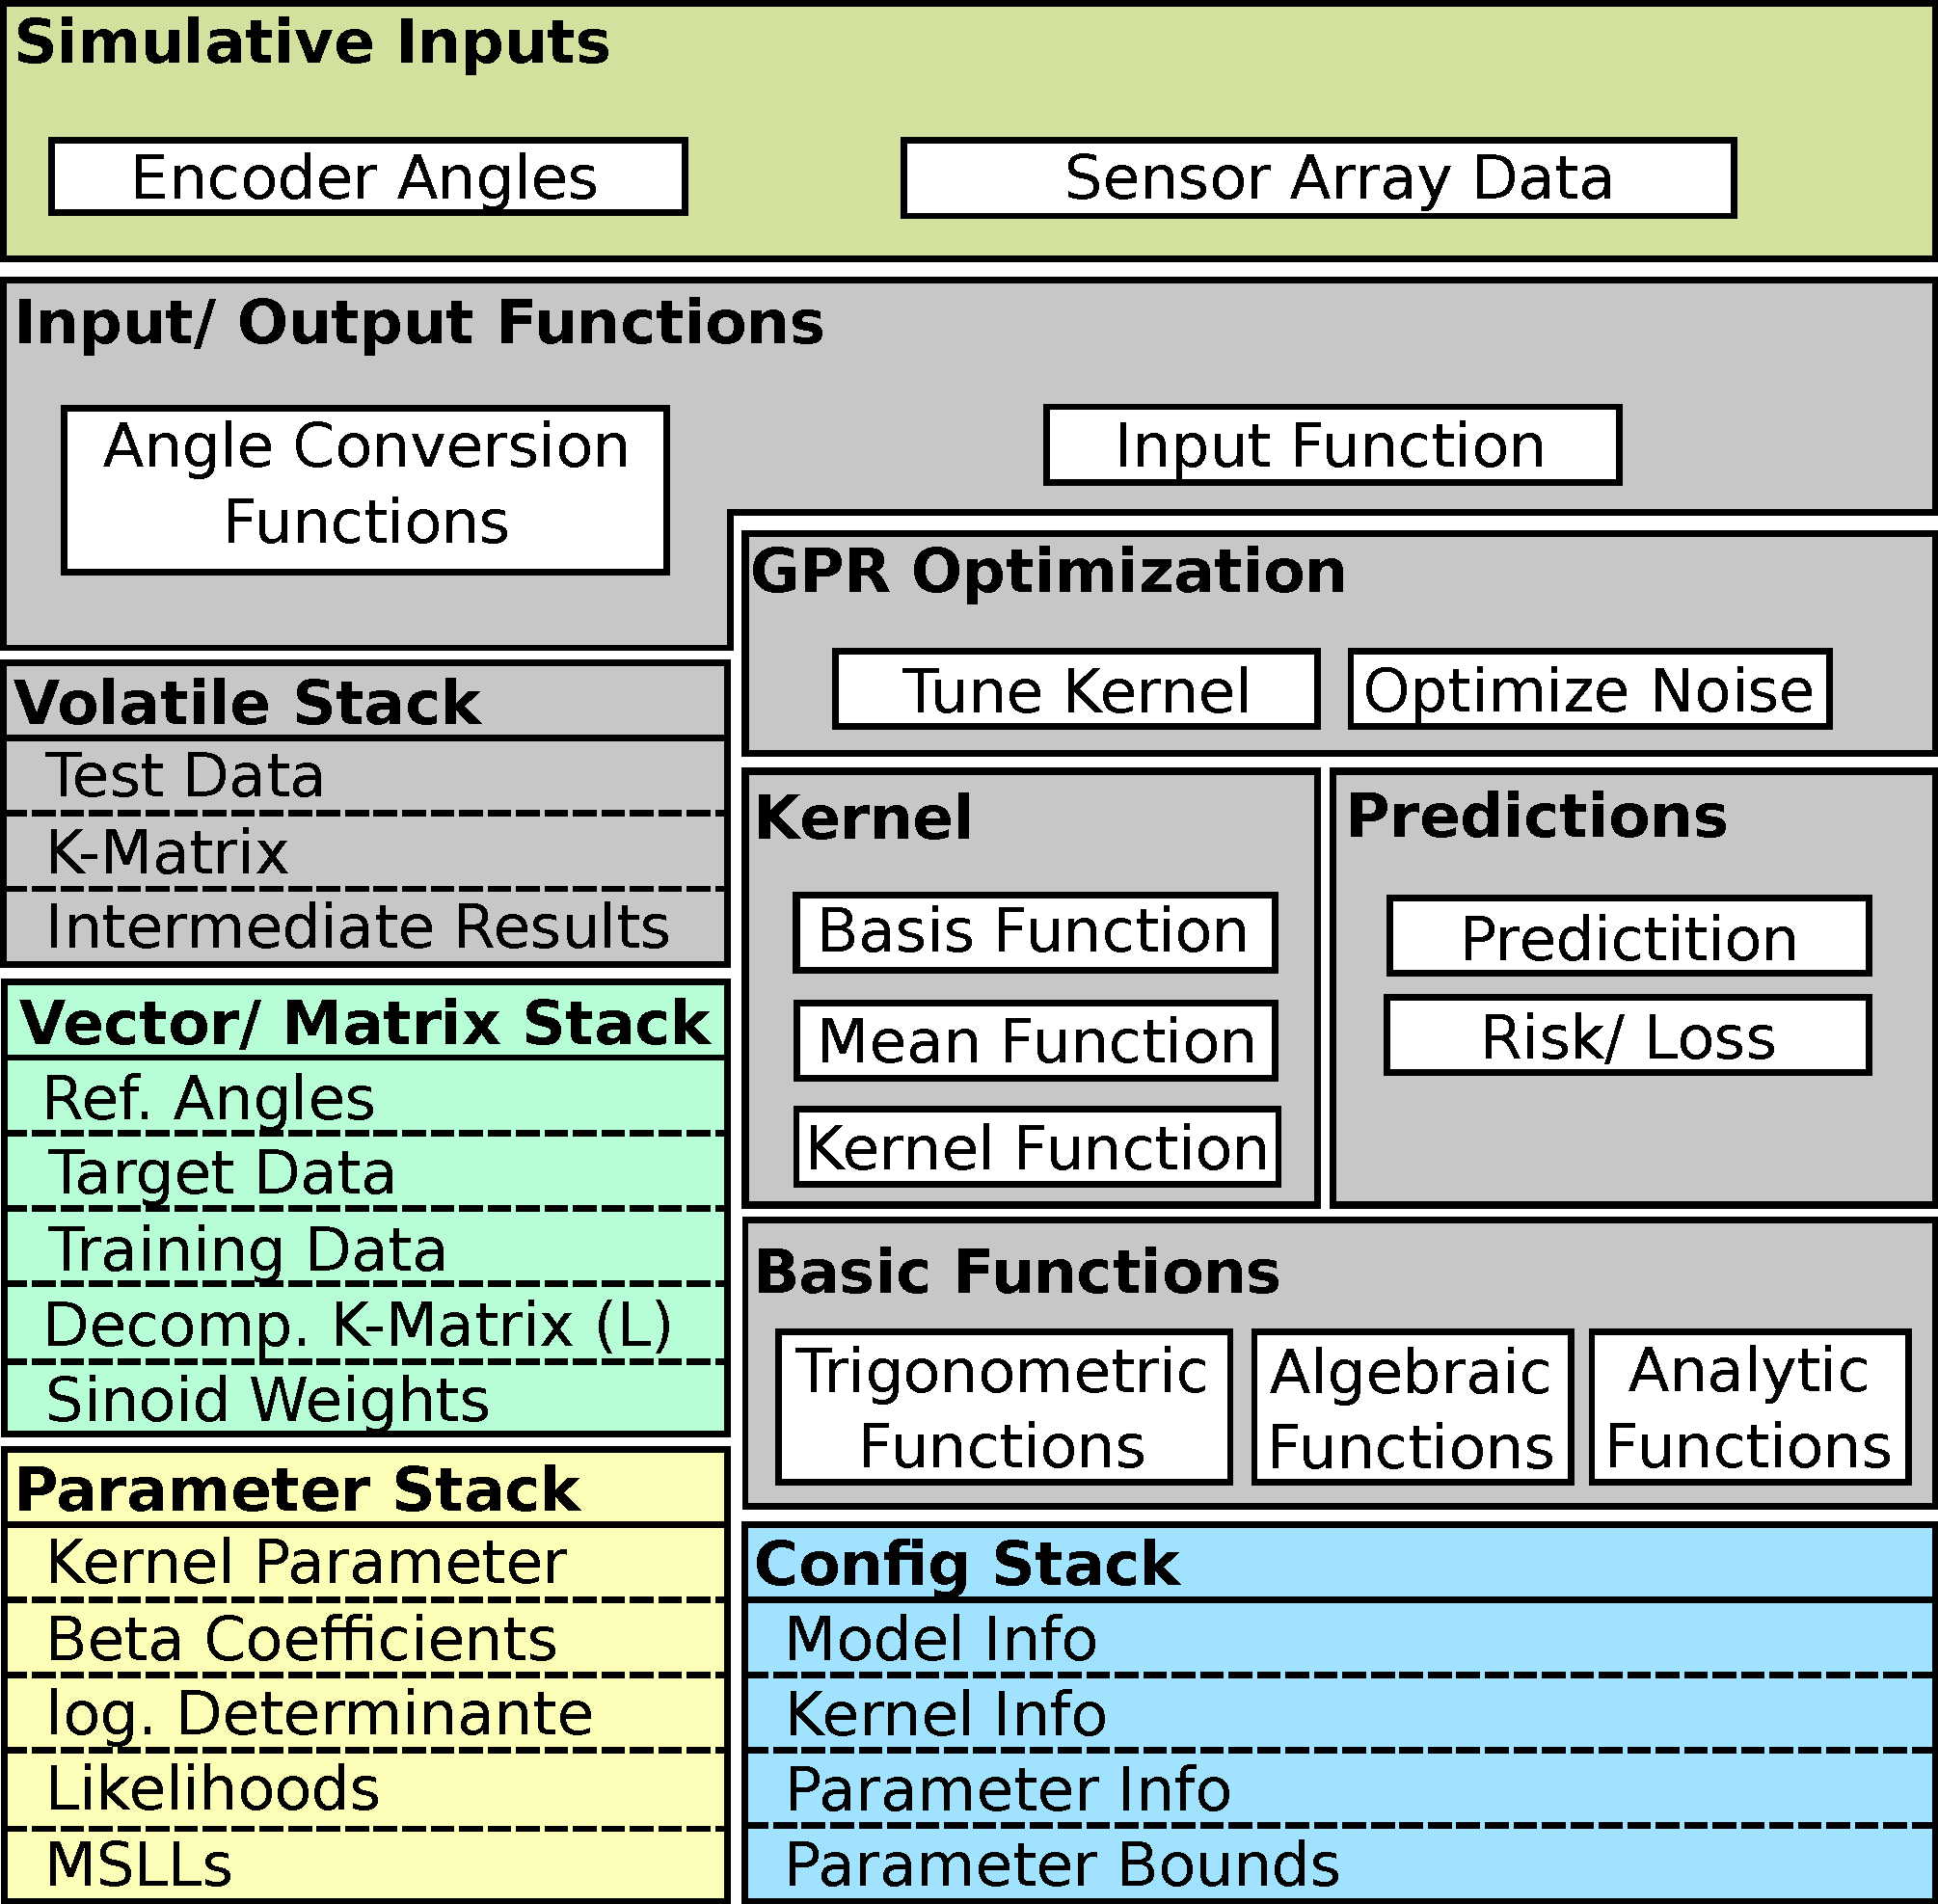
\includegraphics[width=0.7\linewidth]{chapters/images/3-SW-E-OExp/Blockschema_Trainingsphase}
	\caption[Blockschema Trainingsphase Regression]{Blockschema Trainingsphase Regression}
	\label{fig:blockschematrainingsphase}
\end{figure}


\clearpage


\begin{figure}[tbph]
	\centering
	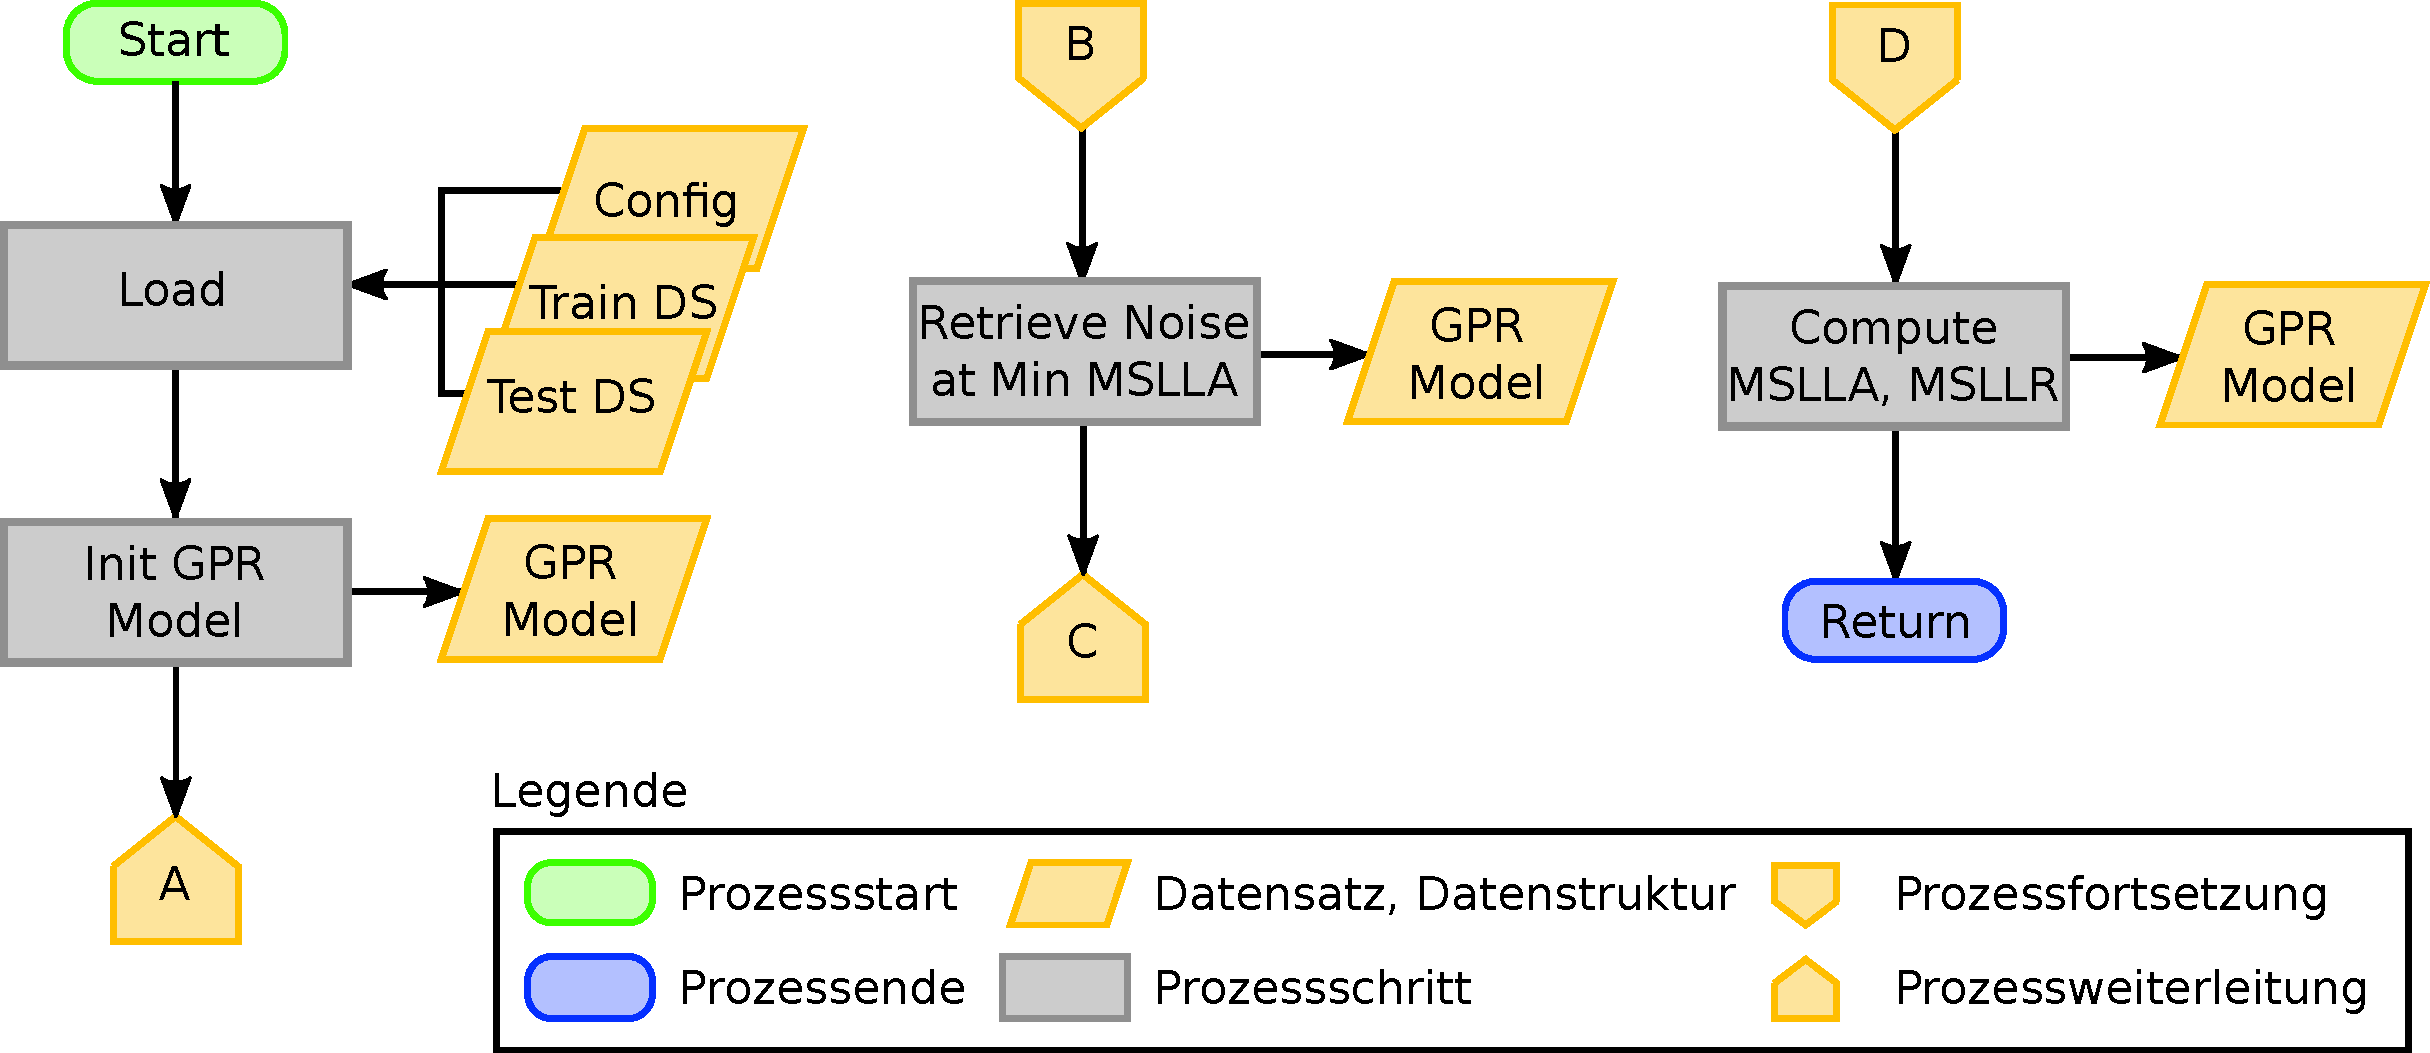
\includegraphics[width=.8\linewidth]{chapters/images/3-SW-E-OExp/GPR_Optimization}
	\caption[Regressionsoptimierung/ -Generalisierung Prozessansicht]{Regressionsoptimierung/ -Generalisierung Prozessansicht}
	\label{fig:gproptimization}
\end{figure}


\clearpage


\begin{figure}[htbp]
	\centering
	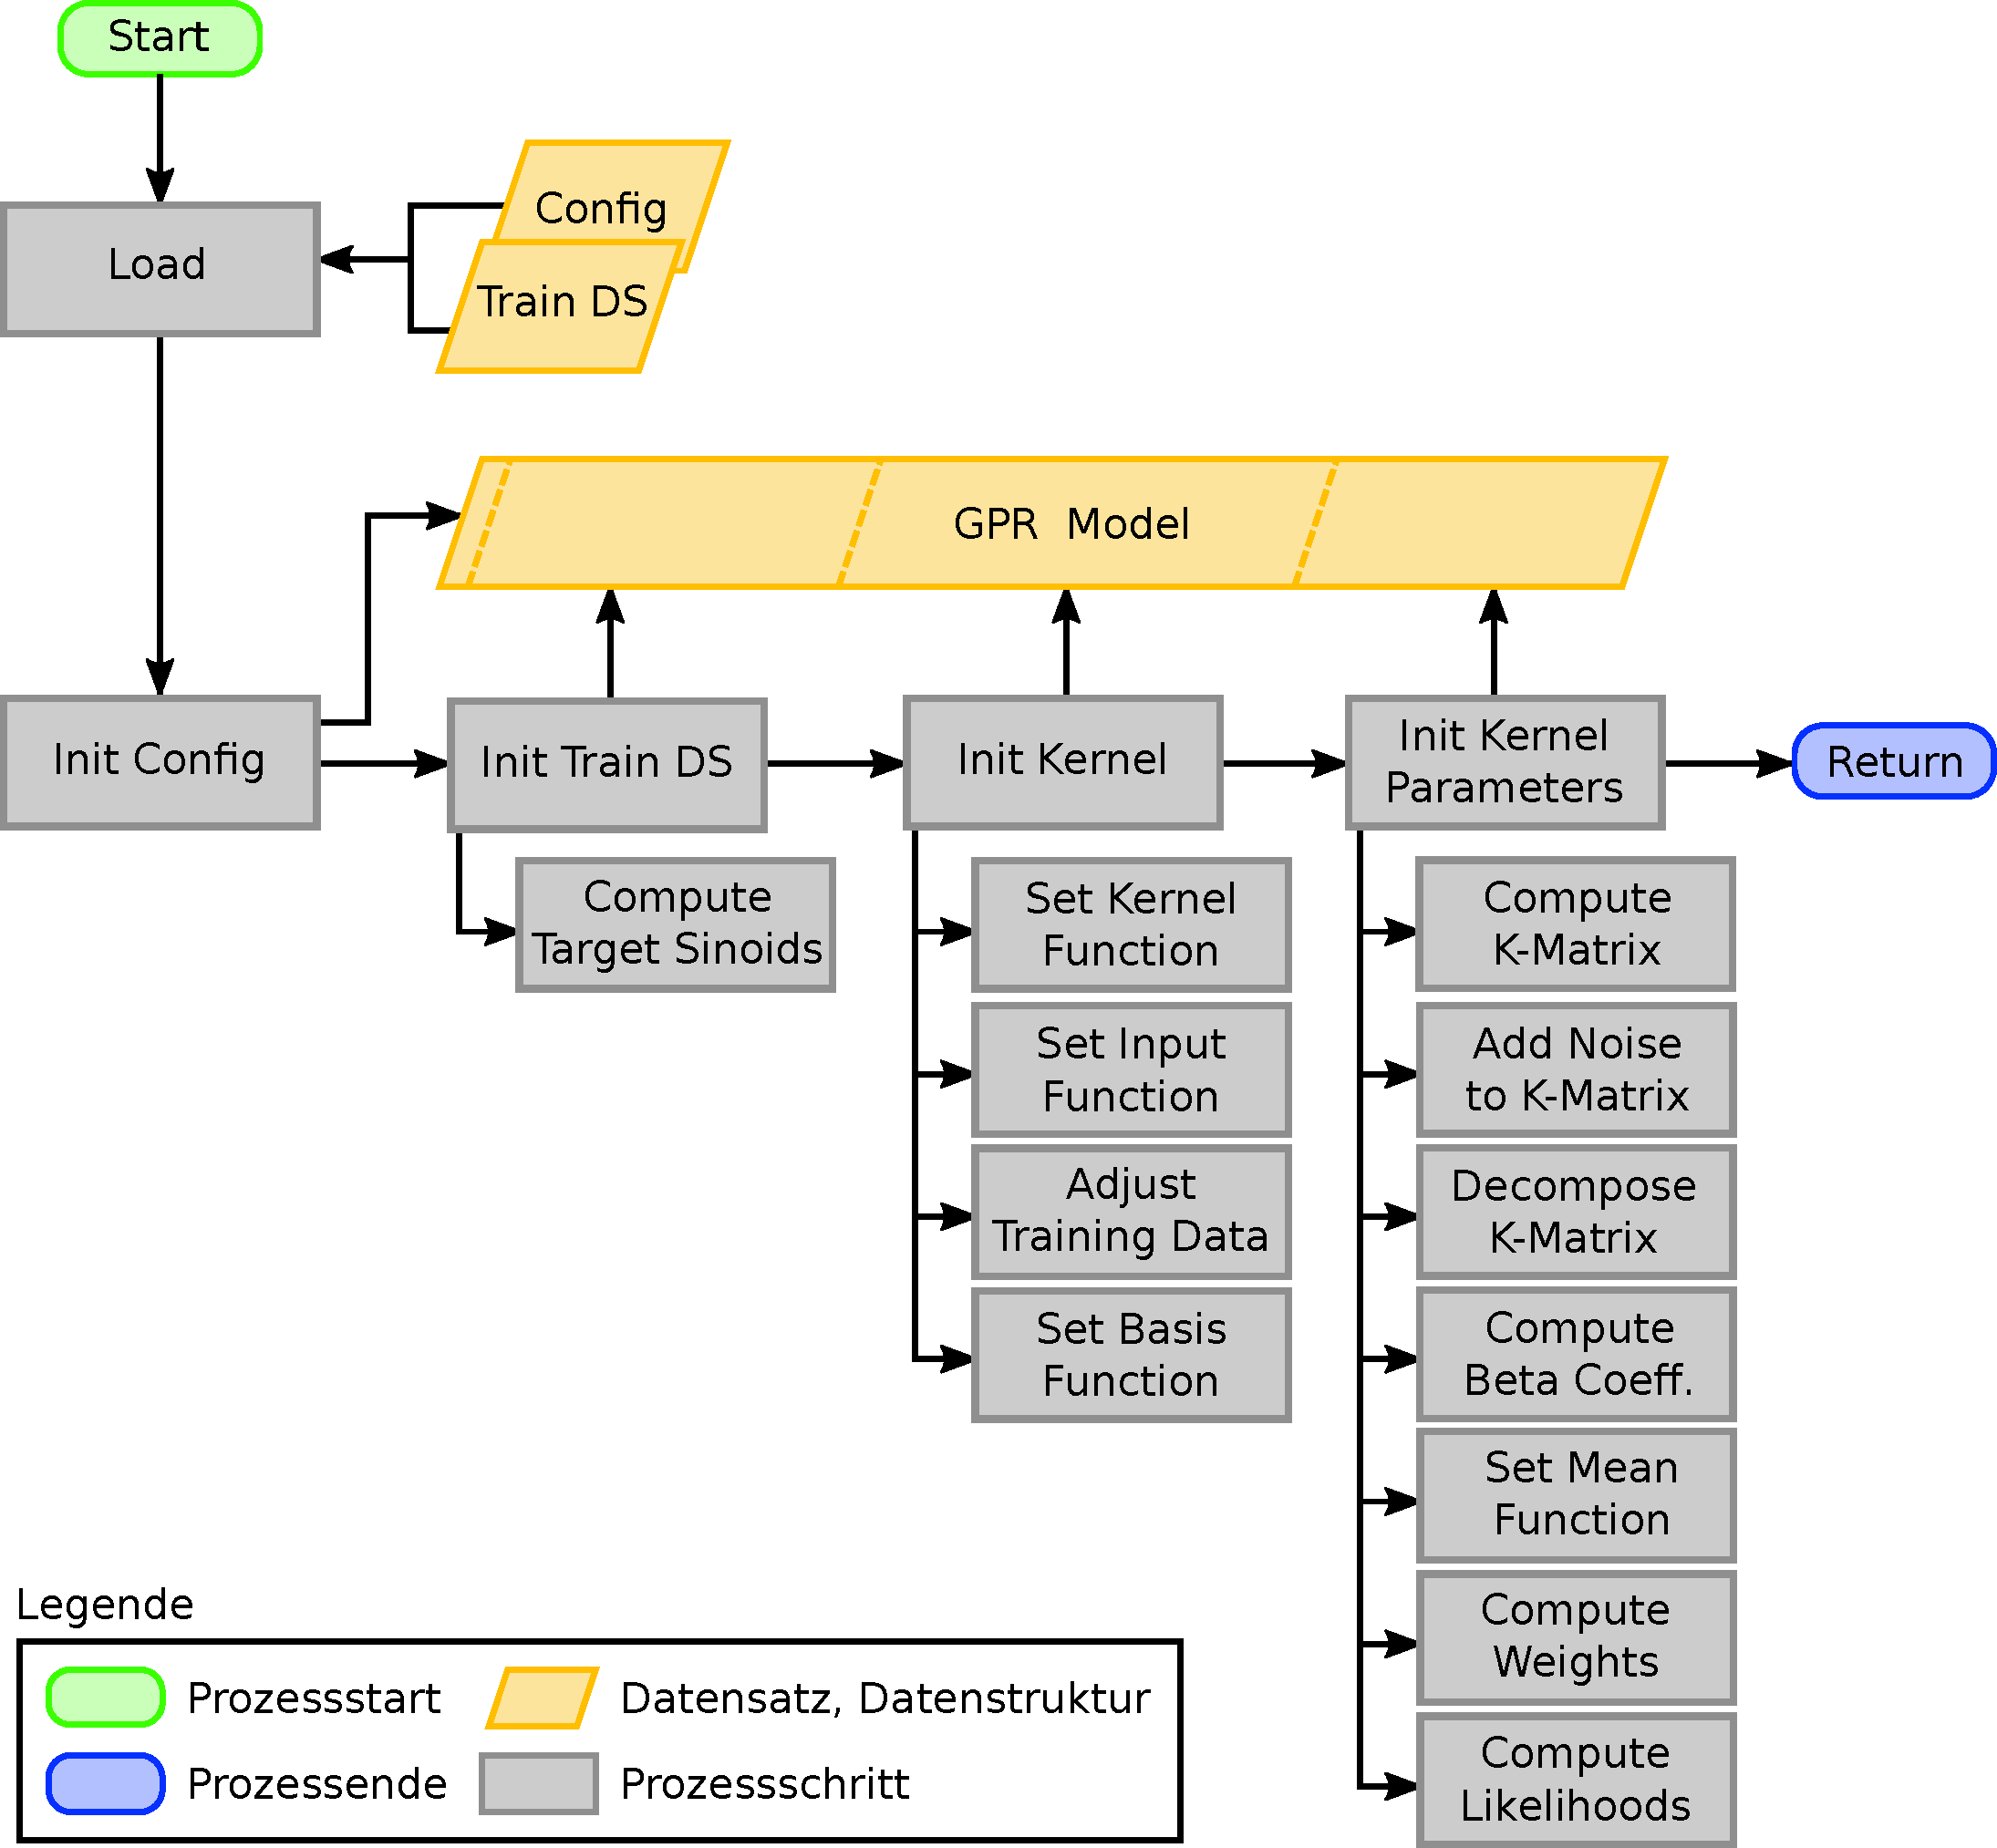
\includegraphics[width=0.7\linewidth]{chapters/images/3-SW-E-OExp/GPR_Initialization}
	\caption[Regressionsinitialisierung Prozessansicht]{Regressionsinitialisierung Prozessansicht}
	\label{fig:gprinitialization}
\end{figure}


\clearpage


\begin{figure}[tbph]
	\centering
	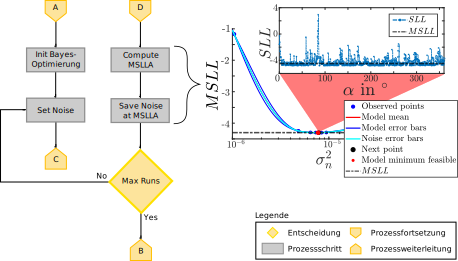
\includegraphics[width=0.85\linewidth]{chapters/images/3-SW-E-OExp/Noise_Optimization}
	\caption[Rauschniveauoptimierung Prozessansicht]{Rauschniveauoptimierung Prozessansicht}
	\label{fig:noiseoptimization}
\end{figure}


\clearpage


\begin{figure}[tbph]
	\centering
	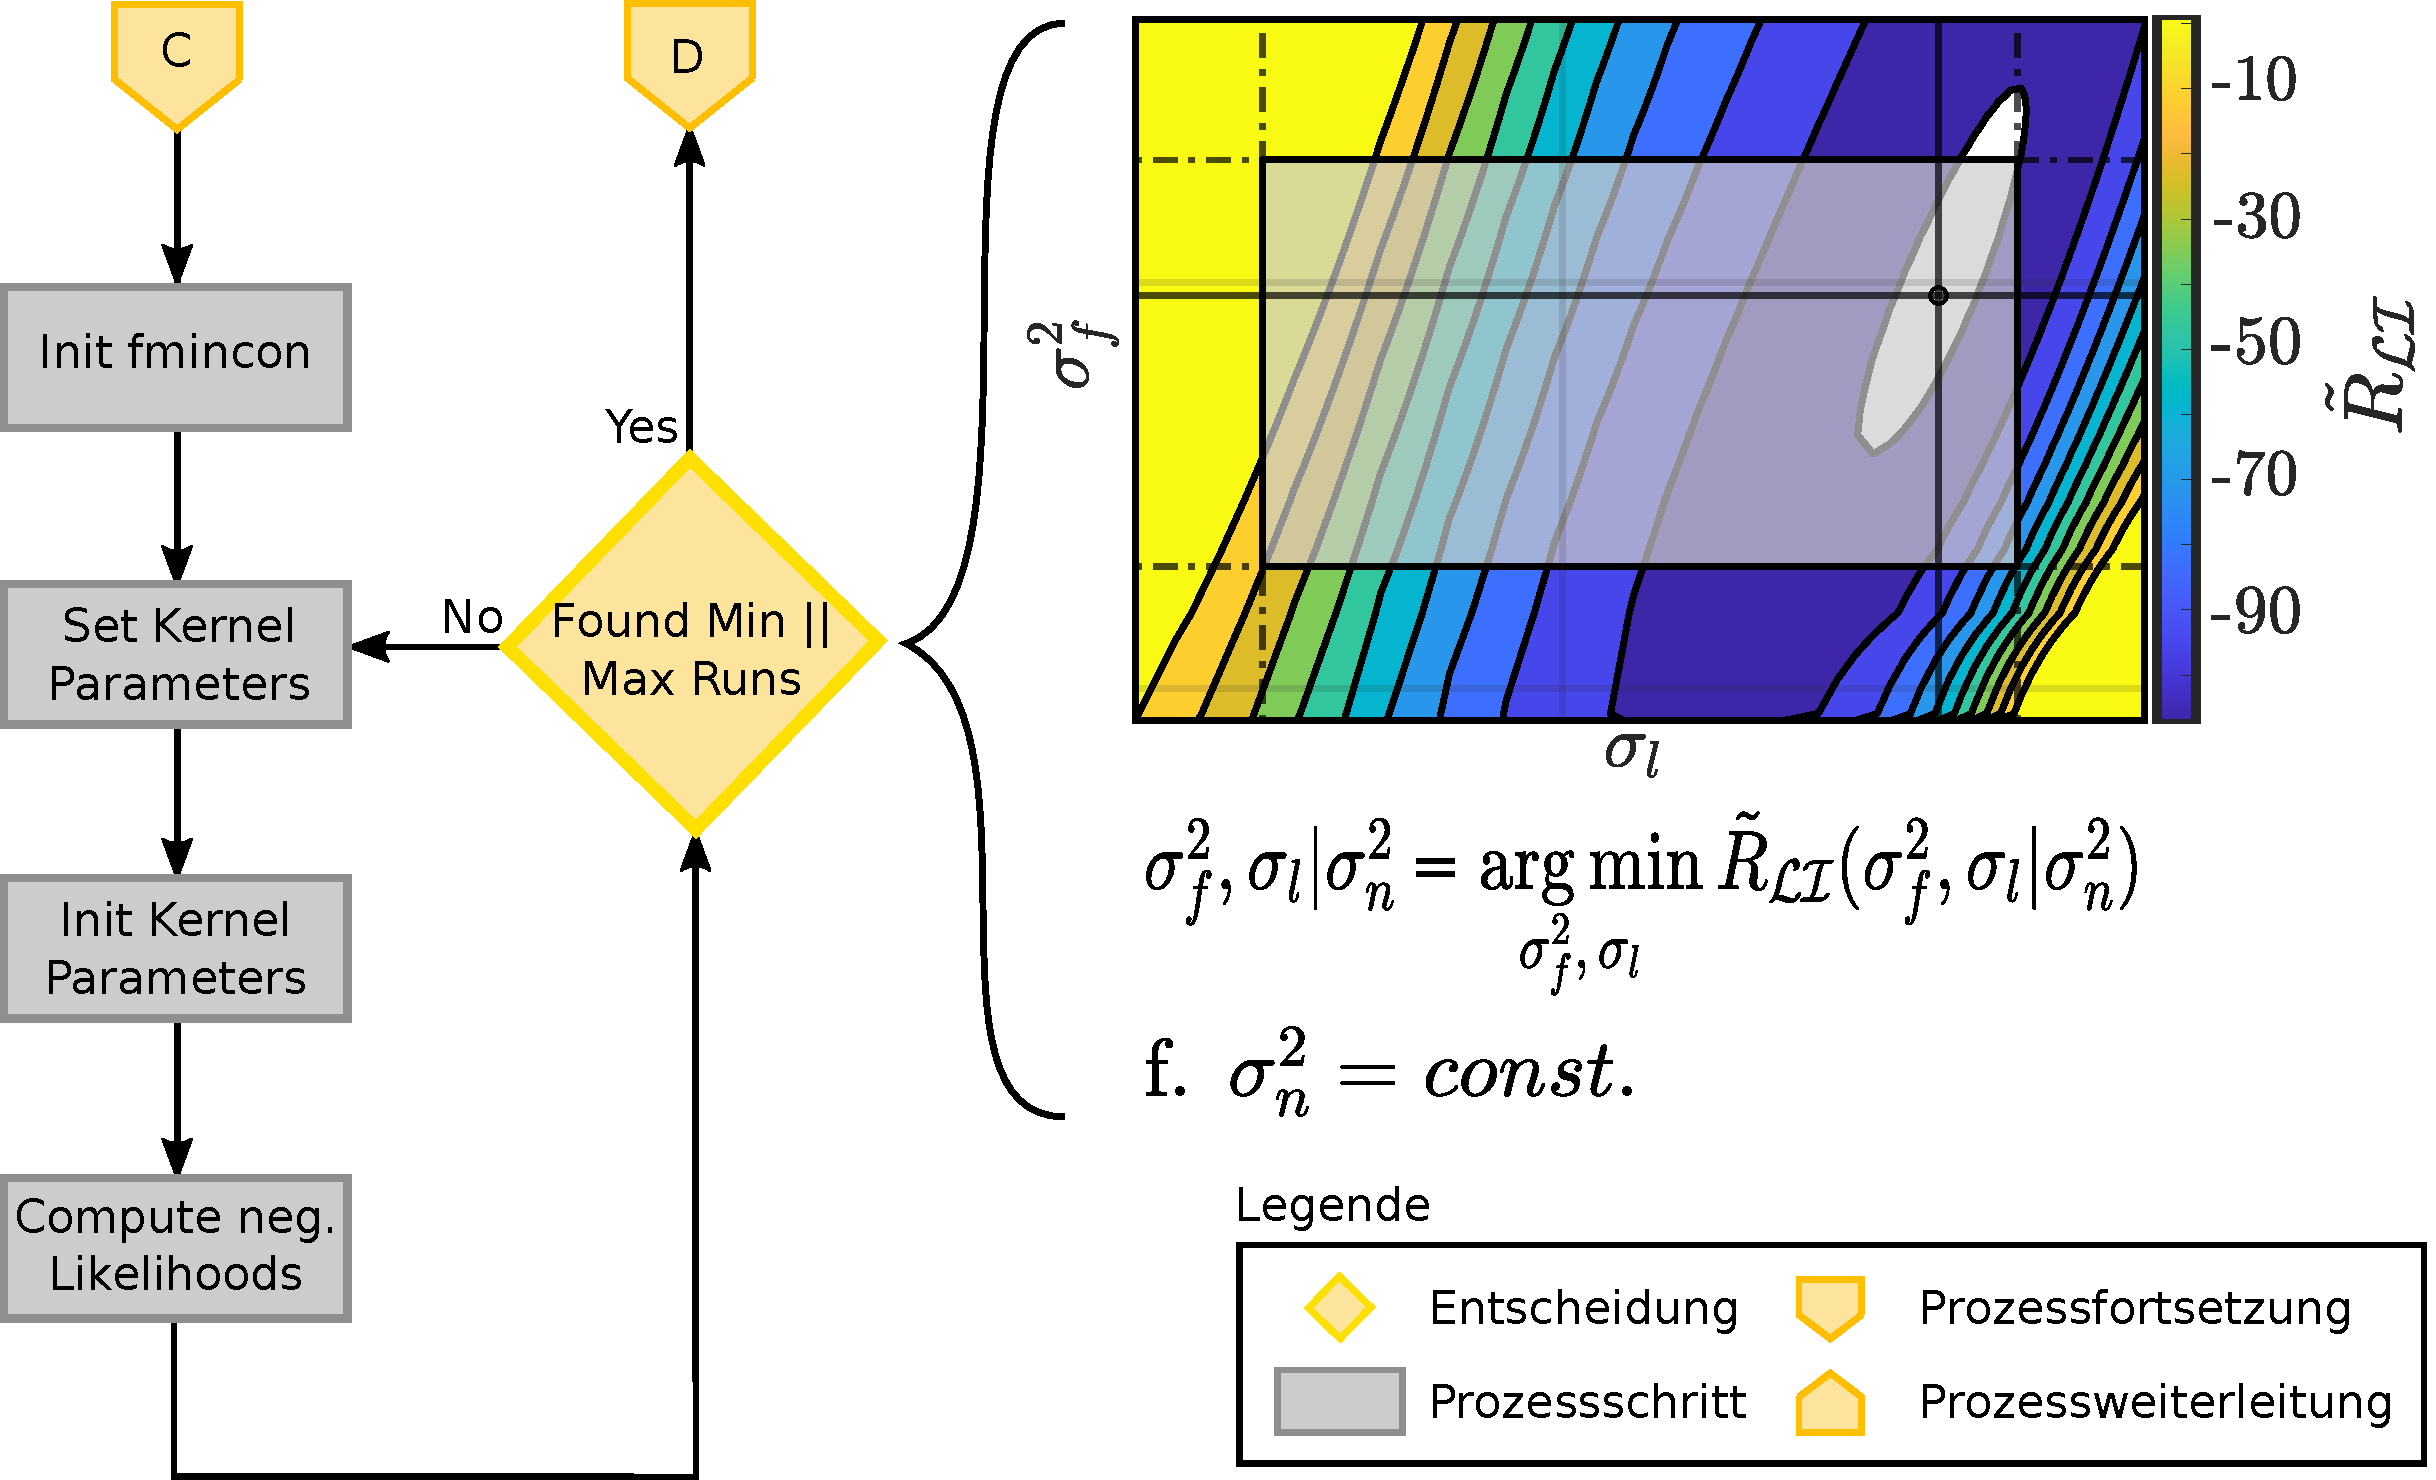
\includegraphics[width=0.8\linewidth]{chapters/images/3-SW-E-OExp/Kernel_Tuning}
	\caption[Regressionsparameteroptimierung Prozessansicht]{Regressionsparameteroptimierung Prozessansicht}
	\label{fig:kerneltuning}
\end{figure}


\clearpage


\paragraph{Arbeitsphase}\label{par:gpr-work-pro}$~$\\


\begin{figure}[tbph]
	\centering
	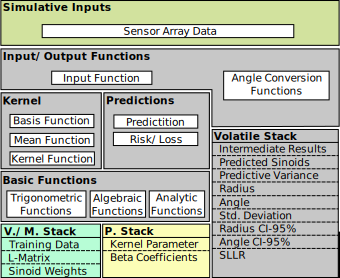
\includegraphics[width=0.7\linewidth]{chapters/images/3-SW-E-OExp/Blockschema_Workphase}
	\caption[Blockschema Arbeitsphase Regression]{Blockschema Arbeitsphase Regression}
	\label{fig:blockschemaworkphase}
\end{figure}


% !TEX root = ../thesis.tex
% testing and optimization experiments
% @author Tobias Wulf
%

\chapter{Erprobungs- und Optimierungsexperimente 0.0.2 26.04.2021}\label{ch:erprobungs-u-opt-exp}
	
	
\section{Vergleich der Kovarianzfunktionen}\label{sec:exp1}


\section{Anpassung der Referenzwinkelanzahl}\label{sec:exp2}


\section{Anpassung des Rauschniveaus}\label{sec:exp3}


\section{Anpassung der Parametergrenzen}\label{sec:exp4}


\section{Verhalten bei einfachen Fehllagen}\label{sec:exp5}
	
%	\begin{itemize}
%		\item Klassifizierung (Diagnose)
%		\item Stabilitätskriterium
%		\item Fehlererkennung Max. Mittelwert, Qualitätsmaß
%		\item Allg. Vorgehen "Batch-Job"
%		\item Konfigurierung der Simulationssoftware
%		\item Kategorisieren von Fehllagen, standardisierbar, mediale, maximale
%		\item Regressionsgrenzen durch Array-Technologie, Dämpfung Ellipsen
%	\end{itemize}
%
%\section{Festlegung des Startpunktes}\label{sec:festlegung-des-startpunktes}
%	\begin{itemize}
%		\item Startpunkt, 1. Position gleich Anlernpunkt für Trainingsphase
%		\item Auswahl des Senortyps
%		\item Konfigurierung des Magneten
%		\item Auswahl des GPR-Modells nach Optimierung
%		\item Konfigurierung des GPR-Modells mit ermittelten Parametern
%	\end{itemize}
%
%
%
%
%\section{Festlegung des Verfahrweges ohne Verkippung}\label{sec:festlegung-verfahrwe-ohne-verkippung}
%	\begin{itemize}
%		\item Vorbetrachtung des Magnetsfeldes 
%		\item Aufteilung in Sektoren
%		\item Abfahren in Z-Richtung ohne Versatz
%		\item Festlegen des X-Y-Versatzes, Symmetrie-Sektor		
%	\end{itemize}
%
%\section{Simulationsdurchführung}\label{sec:simulationsdurchfuehrung}
%	\begin{itemize}
%		\item Festhalten der Ergebnisse
%		\item Position, Winkelfehler (Max, Mittel), Qualitätsmaß (Max, Mittel)
%		\item Drift-Darstellung
%	\end{itemize}
	

% !TEX root = ../thesis.tex
% evaluation
% @author Tobias Wulf
%

\chapter{Auswertung}\label{ch:auswertung}

\section{Gegenüberstellung der GPR-Modelle}\label{sec:gegenueberstellung-gpr-modelle}
	\begin{itemize}
		\item Aufwand der Trainingsphase
		\item Nötige Parameter und zu Speichernde Werte
		\item Arbeitsphase, Genauigkeit, Fehlererkennung, Stabilität
	\end{itemize}
% !TEX root = ../thesis.tex
% summary and conclusion
% @author Tobias Wulf
%

\chapter{Zusammenfassung und Bewertung 0.0.1 13.01.2021}\label{ch:zusammenfassung}
\begin{itemize}
	\item Kurzdarstellung der Ergebnisse der Arbeit
	\item Offene Punkte und Probleme
	\item Ansätze zur Weiterführung für zukünftige Arbeiten
	\item Bewertung der Ergebnisse in Bezug auf die Anwendung
\end{itemize}


% List of figures here
\clearpage
\IListOfFigures

% List of tables here
\clearpage
\IListOfTables

% List of algorithms here
\clearpage
\renewcommand{\listalgorithmcfname}{Algorithmenverzeichnis}
\listofalgorithms
\addcontentsline{toc}{chapter}{Algorithmenverzeichnis}

% List glossary entries
\clearpage
\IGlossary

% List of accronyms here
\clearpage
\IListOfAccronyms

% List of symbols here
%\clearpage
%\IListOfSymbols

% List of used literature
\nocite{*}
\printbibliography
%\printbibliography[nottype=online, keyword={paper}, heading=subbibliography, title={Paper}]
%\printbibliography[nottype=online, keyword={thesis}, heading=subbibliography, title={Thesis}]
%\printbibliography[nottype=online, keyword={manual}, heading=subbibliography, title={Manual}]
%\printbibliography[type=online, keyword={webpage}, heading=subbibliography, title={Web-Recherche}]
% \bibliographystyle{plain}
%\bibliographystyle{dinat}
%\bibliography{literature/literature}

% Appendix
\cleardoublepage
\phantomsection
\appendix
\addcontentsline{toc}{part}{\appendixname}
\addtocontents{toc}{\protect\setcounter{tocdepth}{6}}
\setcounter{secnumdepth}{5}
% !TEX root = ../thesis.tex
% appendix TDK TAS2141-AAAB char dataset
% @author Tobias Wulf
%

\chapter{TDK TAS2141-AAAB Kennfelddatensatz 0.0.1 29.03.2021}\label{ch:tdk-datensatz}

Der Anhang beinhaltet die Kennfelddarstellung eines TAS2141-AAAB TMR-Winkelsensor der Firma TDK \cite{TDK2016}. Die 
Charakterisierung des Sensor-ICs ist mittels Kennfeldmethode \cite{Schuethe2019} vorgenommen worden. Das Ausmessen des 
TMR-Sensors hat im Labor der \gls{gl:ags} stattgefunden. Als Charakterisierungsergebnis liegt entsprechender Datensatz 
vor und dient in dieser Arbeit als Simulationsgrundlage für die Sensor-Array-Simulation. Der Datensatz ist von der 
\gls{gl:ags} zur Verfügung gestellt worden.


\vspace{5mm}
\begin{table}[!htbp]
	\centering
	%\resizebox{\textwidth}{!}{
	\begin{tabular}{l l l}
		\toprule
		\textbf{Eigenschaft}      & \textbf{Wert}    & \textbf{Einheit} \\
		\midrule
		$H_x$-Skala               & $-25 \ldots 25$  & $\SI{}{\kilo\ampere\per\metre}$ \\
		$H_y$-Skala               & $-25 \ldots 25$  & $\SI{}{\kilo\ampere\per\metre}$ \\
		\hline
		$H_x$-Schrittweite        & $0,1961$         & $\SI{}{\kilo\ampere\per\metre}$ \\
		$H_y$-Schrittweite        & $0,1961$         & $\SI{}{\kilo\ampere\per\metre}$ \\
		\hline
		Auflösung                 & $256 \times 256$ & Pixel \\
		Wertebereich $V(H_x,H_y)$ & Normiert         & $\SI{}{\milli\volt\per\volt}$ \\
		\hline
		Normfaktor                & $1\cdot 10^{-3}$ & $\SI{}{\per\milli\volt}$ \\
		Gain                      & 1                & - \\
		\hline
		Brückenverdrehung         & 90               & $\SI{}{\degree}$ \\
		Periodizität              & 360              & $\SI{}{\degree}$ \\
		\bottomrule		
	\end{tabular}%}
	\caption[Eckdaten TDK TAS2141-AAAB Kennfelder]{Eckdaten TDK TAS2141-AAAB Kennfelder}
\label{tab:tdk-char-data}
\end{table}


Die Charakterisierung mittels Kennfeldmethode generiert zwei Kennfeldpaare, zu sehen in \autoref{fig:tdkkennfelder}. 
Das erste Kennfeldpaar a) und c) referenziert sich aus dem steigenden Messverlauf, der amplitudenmodulierten 
$H_x$-/ $H_y$-Stimuli. Das zweite b) und d) setzt sich aus dem fallenden Stimuli zusammen. Ein Kennfeld repräsentiert 
dabei eine Wheatstone-Brücke des Winkelsensors \cite{Schuethe2019}. Bedingt durch die Verdrehung beider Brücken 
\cite{TDK2016}, ist ein entsprechendes Kennfeldpaar zueinander um $\SI{90}{\degree}$ verdreht.
Die Kennfelder besitzen, je ein Minimum und Maximum, dass bei Abfahren eines Kreises auf einem Kennfeld zur 
$\SI{360}{\degree}$ Periodizität führt. Die Kennfelder entsprechen somit dem Kernverhalten des Winkelsensors 
\cite{TDK2016}. \autoref{tab:tdk-char-data} fasst die Grundeigenschaften der Kennfelder zusammen. Beim zusammensetzen 
der Kennfelder, sind die gemessen Ausgangsspannungen normiert und von Offsets bereinigt worden. Das erleichtert den 
Simulationseinsatz mit variablen Betriebsspannungen. So können für beliebige Feldstärken, Ausgangsspannungen nach 
\autoref{eq:vout-tdk} aus den Kennfeldern entnommen werden.


\begin{equation}\label{eq:vout-tdk}
	\mathbf{V_{cos,sin}(H_x,H_y) = Gain \cdot Normfaktor \cdot V(H_x,H_y) \cdot V_{CC} + V_{Offset}}
\end{equation}


\begin{figure}[bph]
	\centering
	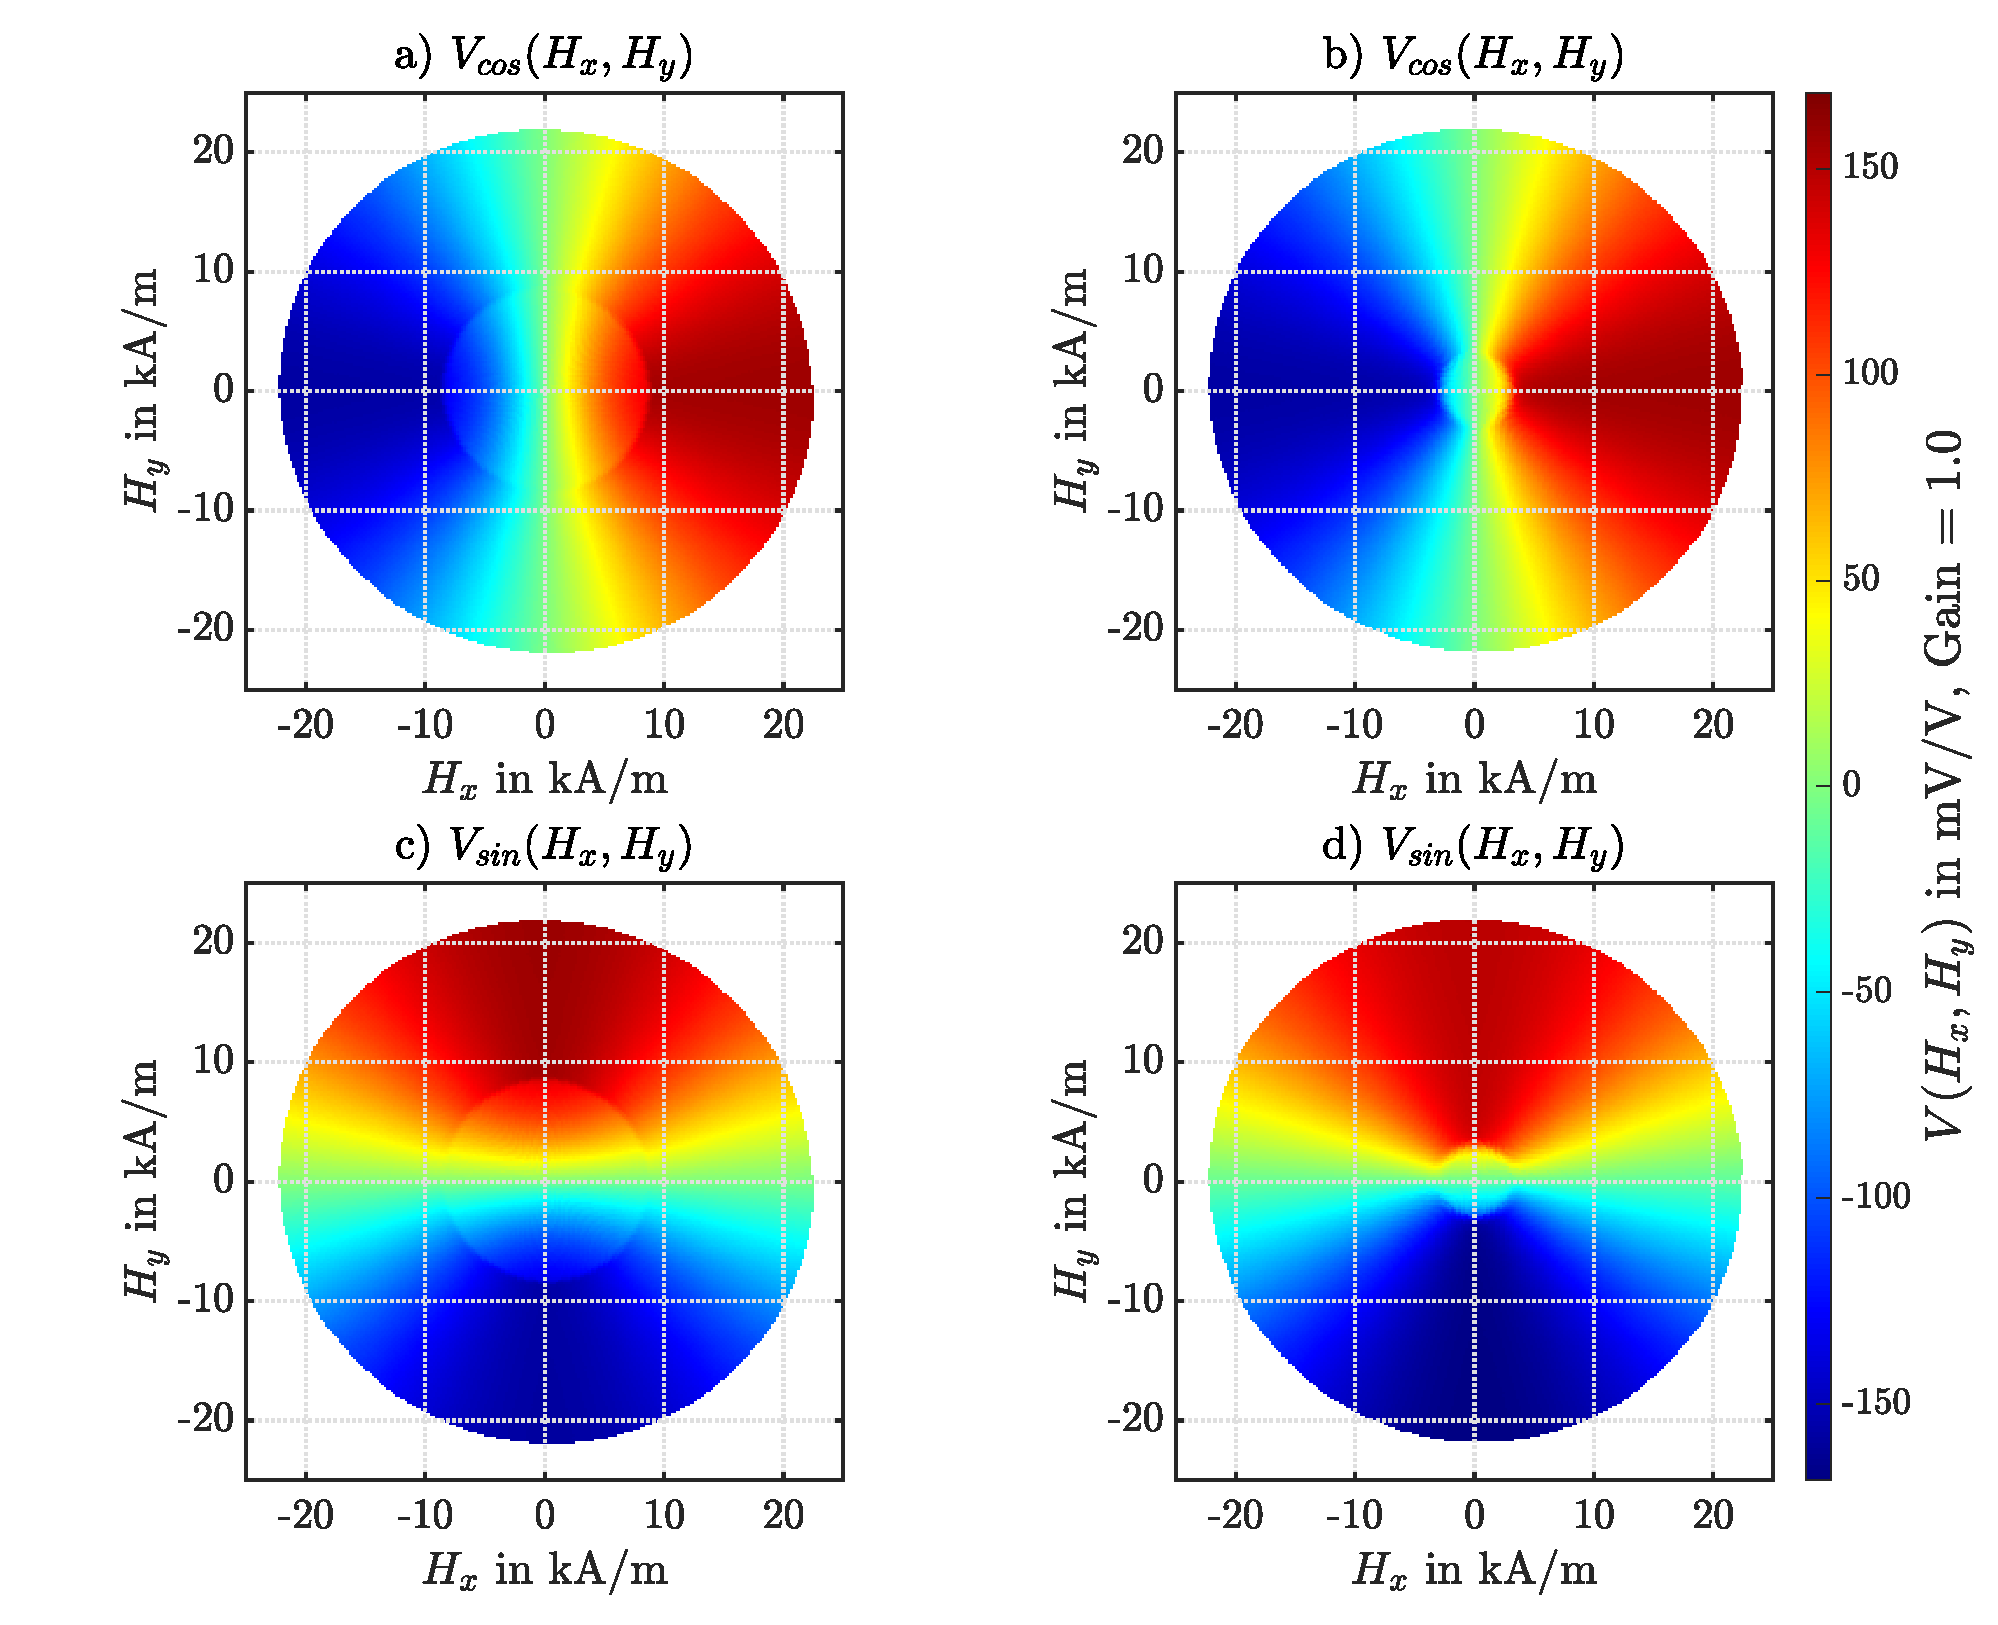
\includegraphics[width=.95\linewidth]{appendix/images/3-TDK/TDK_Kennfelder}
	\caption[TDK TAS2141-AAAB Brückenkennfelder]{TDK TAS2141-AAAB Brückenkennfelder. Kennfelder der Cosinus-Brücke a) 
		und b). Kennfelder der Sinus-Brücke c) und d). a) und c) gewonnen aus steigenden Amplitudenmodulation. b) und 
		d) gewonnen fallenden Modulation. Die Kennfelder sind normiert in $\SI{}{\milli\volt\per\volt}$. Grafik 
		nachempfunden 
		aus \cite{Schuethe2019}.}
	\label{fig:tdkkennfelder}
\end{figure}


\clearpage


Im Vergleich der Kennfeldpaare biete sich das erste aus aus \autoref{fig:tdkkennfelder} a) und c) für eine Simulation 
an. Die Kennfelder besitzen größere Plateauflächen \cite{Schuethe2019}. In \autoref{fig:tdkkennfeldsteigend} a) und c) 
ist das Kennfeldpaar nochmals gesondert dargestellt. Für das Kennfeld, der Cosinus-Wheatstone-Brücke in a), sind 
Querschnitte für variable $H_x$- und verschieden konstante $H_y$-Feldstärken in b) aufgetragen. Das gleiche vice versa 
in d) für Sinus-Wheatstone-Brücke aus c). Die Plateau-Grenzen liegen in $H_x$- und $H_y$-Richtung ca. bei 
$\pm\SI{8,5}{\kilo\ampere\per\metre}$ und sind als Limits in \autoref{fig:tdkkennfeldsteigend} b) und d) 
gekennzeichnet. Es zeigt sich ein annähernd linearer Bereich für die Übertragungskennlinien bei $H_{x,y} 
= \SI{0}{\kilo\ampere\per\metre}$. Dieser Arbeitsbereich ist für die Simulation einzustellen \cite{Schuethe2019}.


\vspace{5mm}
\begin{figure}[bph]
	\centering
	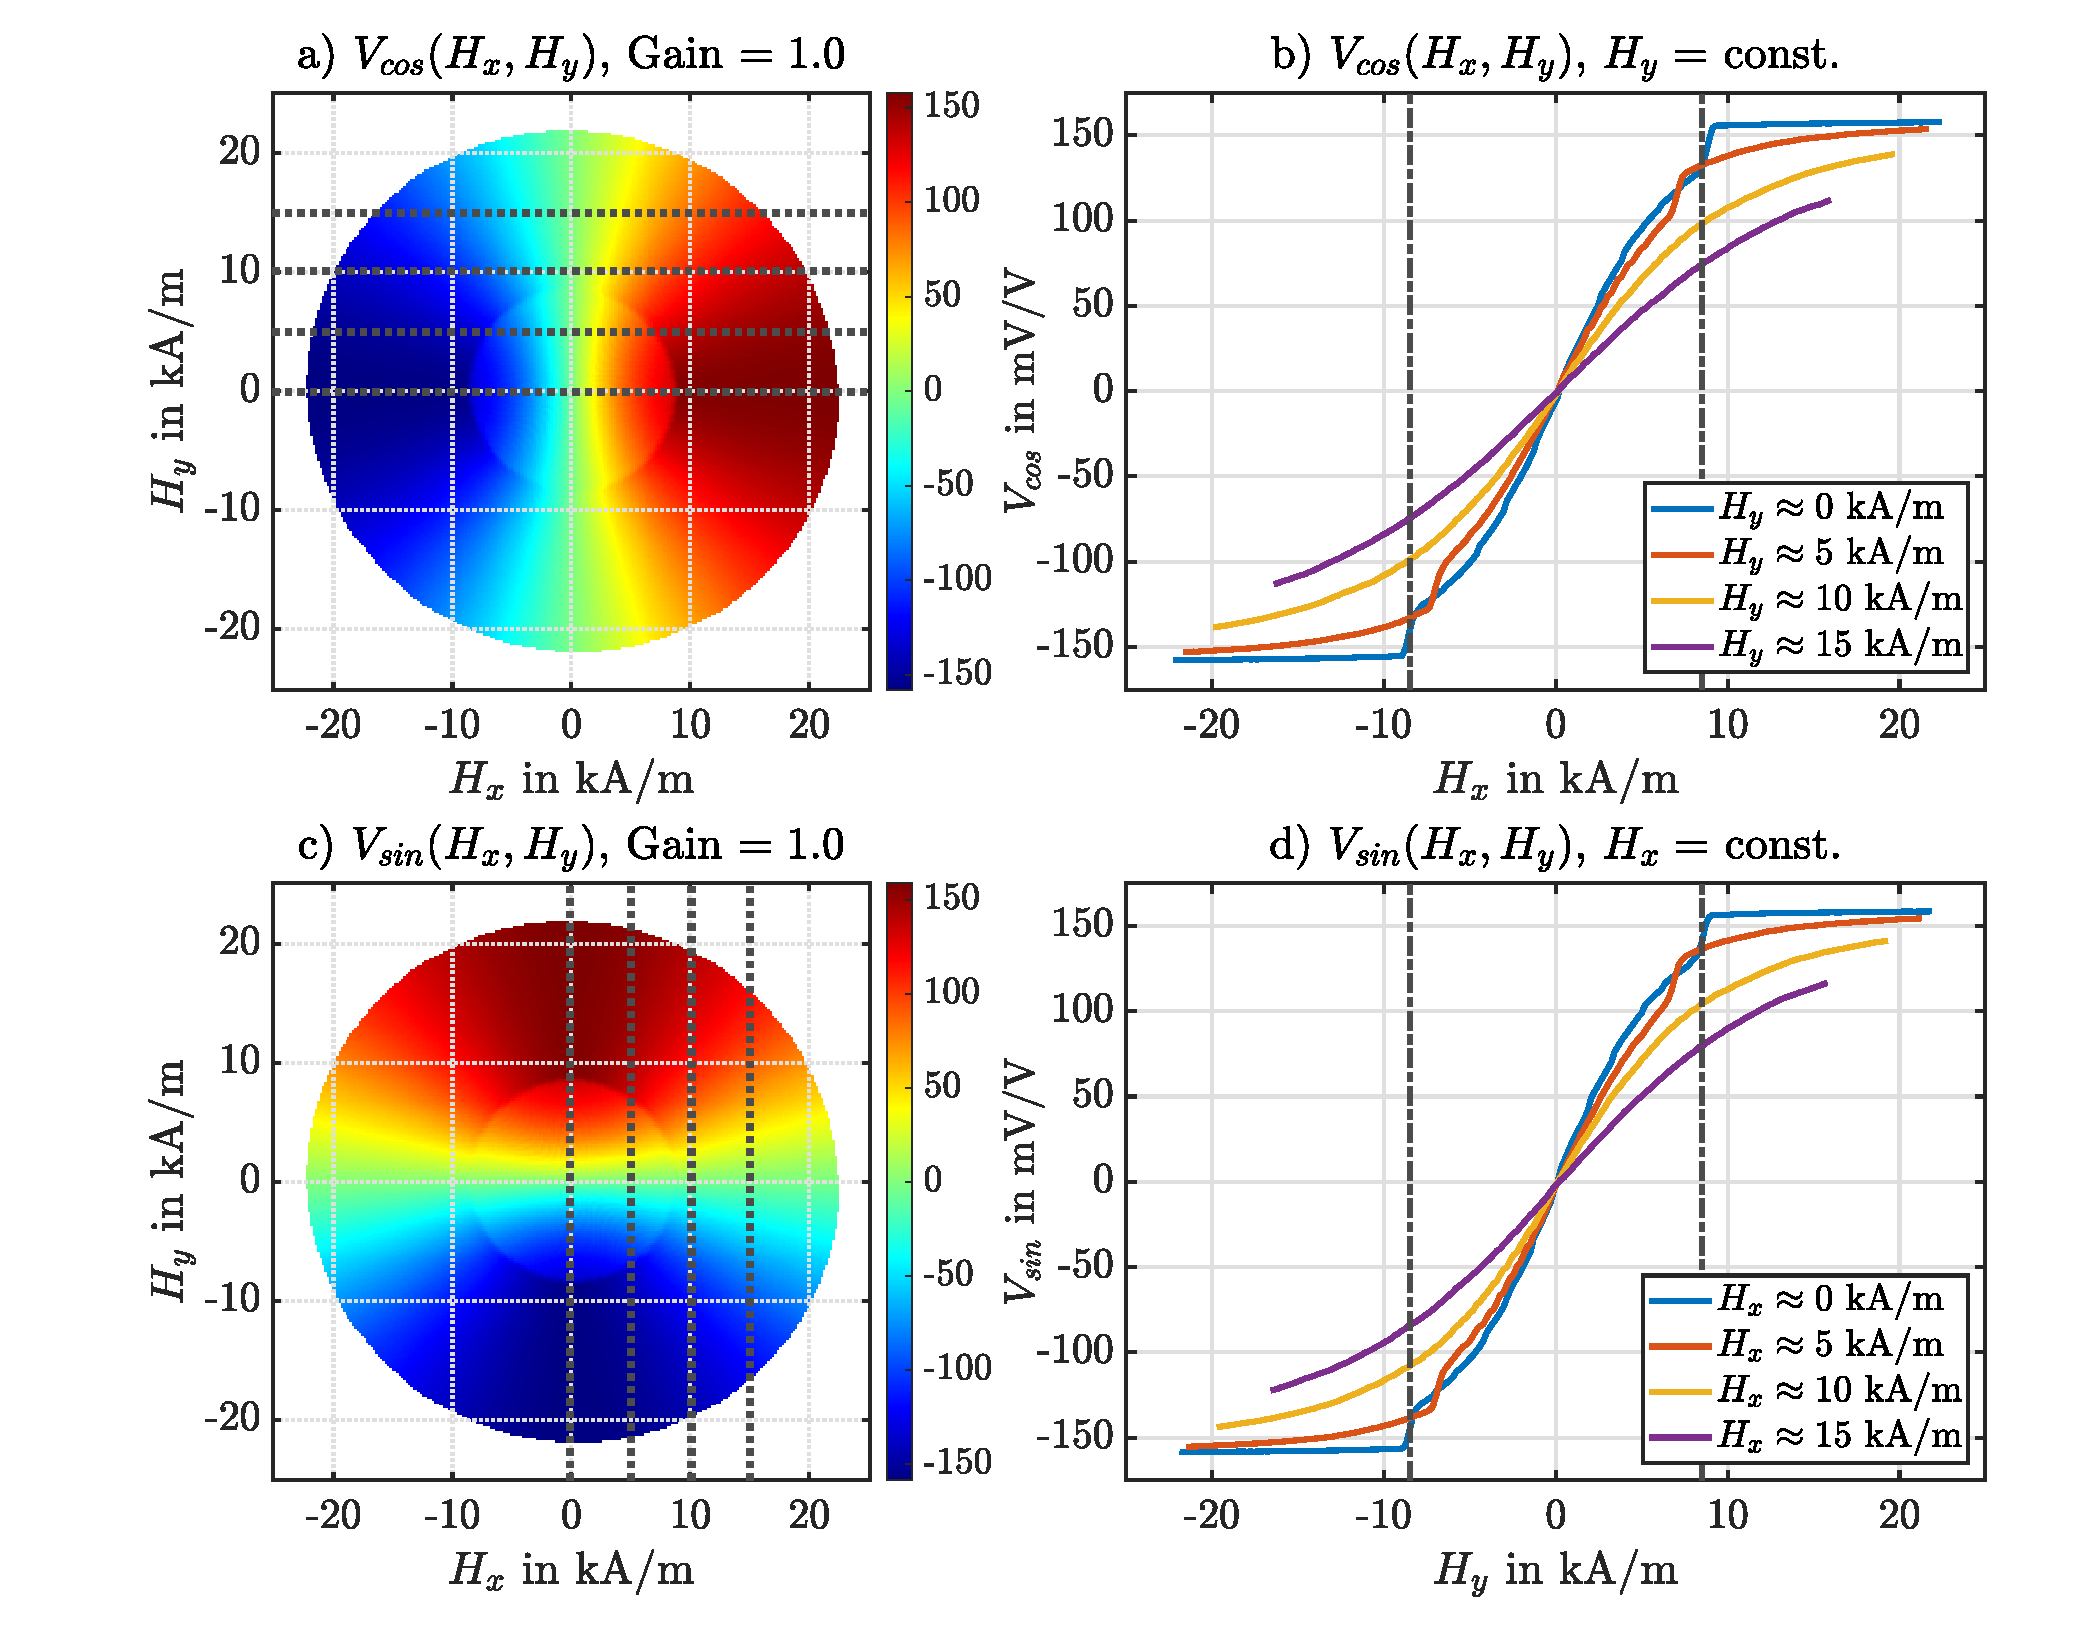
\includegraphics[width=.95\linewidth]{appendix/images/3-TDK/TDK_Kennfeld_Steigend}
	\caption[TDK TAS2141-AAAB Kennfeldquerschnitte]{TDK TAS2141-AAAB Kennfeldquerschnitte. Cosinus-Brücken-Kennfeld in 
	a) und Sinus-Brücke in c). In b) und d) sind folgend der Verdrehung Querschnitte aus a) und c) aufgetragen. In b) 
	$V_{cos}$ f. variable $H_x$- und verschieden konst. $H_y$-Feldstärken. In d) vice versa für $V_{sin}$ mit 
	verschieden konst. $H_x$- bei variablen $H_y$-Feldstärken. Breite lineare Plateaus liefern einen annähernd linearer 
	Arbeitsbereich in c) und d) zw. $\pm\SI{8,5}{\kilo\ampere\per\metre}$ f. Übertragungskennlinien $H_{x,y} = 
	\SI{0}{\kilo\ampere\per\metre}$. Grafik aus \cite{Schuethe2019}.}
	\label{fig:tdkkennfeldsteigend}
\end{figure}

% !TEX root = ../thesis.tex
% appendix Senor Array Simulation
% @author Tobias Wulf
%

\chapter{Sensor-Array-Simulation Implementierung}\label{ch:sensor-array-sim-imp}


Der Anhang veranschaulicht die Handhabung und Standardparametrierung für die Sensor-Array-Simulation. Es sind optimale Simulationsparameter in \autoref{tab:sensor-array-sim-params} aufgeführt. Diese sind im Konfigurationsskript einzustellen und vorab der Simulation auszuführen. Das Skript erstellt eine MAT-Datei. Diese enthält, die in Gruppen zusammengefasste Simulationsparametrierung. Bei Simulationsausführung sind betreffende Parametergruppen aus der Konfigurationsdatei zu laden.


\vspace{5mm}
\begin{table}[!htbp]
	\centering
	\resizebox{\textwidth}{!}{
	\begin{tabular}{l l c c l}
		\toprule
		\textbf{Parametergruppe}                 & \textbf{Parameter} & \textbf{Wert}      & \textbf{Einheit}                & \textbf{Kurzbeschreibung}                       \\ \midrule
		\multirow{6}{*}{SensorArrayOptions}      & geometry           & 'square'           & -                               & Array-Geometrie-Indikator                       \\
		                                         & dimension          & $8$                & -                               & Sensor-Array-Pixel $N_{Pixel} \times N_{Pixel}$ \\
		                                         & edge               & $2$                & $\SI{}{\milli\metre}$           & Sensor-Array-Kantenlänge                        \\
		                                         & $V_{cc}$           & $5$                & $\SI{}{\volt}$                  & Sensor-Array-Betriebsspannung                   \\
		                                         & $V_{off}$          & $2,5$              & $\SI{}{\volt}$                  & Sensor-Brücken-Offset-Spannung                  \\
		                                         & $V_{norm}$         & $1 \cdot 10^3$     & $\SI{}{\milli\volt}$            & Kennfeldnormierung                              \\ \hline
		\multirow{4}{*}{DipoleOptions}           & sphereRadius       & $2$                & $\SI{}{\milli\metre}$           & Kugelmagnetradius                               \\
		                                         & $H_{0mag}$         & $200$              & $\SI{}{\kilo\ampere\per\metre}$ & Betragsfeldstärke Magnetfeldnormierung          \\
		                                         & $z_0$              & $1$                & $\SI{}{\milli\metre}$           & $Z$-Abstand Magnetfeldnormierung                \\
		                                         & $m_{0mag}$         & $1 \cdot 10^6$     & $\SI{}{\ampere\square\metre}$   & Magnitude d. mag. Moments                       \\ \hline
		\multirow{10}{*}{Training-/ TestOptions} & useCase            & 'Training'/ 'Test' & 'char'                          & Datensatzindikator f. Anwendungszweck           \\
		                                         & xPos               & $\left[0,\right]$  & $\SI{}{mm}$                     & Sensor-Array $X$-Positionsvektor                \\
		                                         & yPos               & $\left[0,\right]$  & $\SI{}{mm}$                     & Sensor-Array $Y$-Positionsvektor                \\
		                                         & zPos               & $\left[7,\right]$  & $\SI{}{mm}$                     & Sensor-Array $Z$-Positionsvektor                \\
		                                         & tilt               & $0$                & $\SI{}{\degree}$                & Magnetverkippung in $Y$-Achse                   \\
		                                         & angleRes           & $0,5$              & $\SI{}{\degree}$                & Winkelauflösung f. Magnetrotation               \\
		                                         & phaseIndex         & 0                  & -                               & Phasenverschiebung-Index f. Startwinkel         \\
		                                         & nAngles            & $20$/ $720$        & -                               & Anzahl gleich verteilter Simulationswinkel      \\
		                                         & BaseReference      & 'TDK'              & char                            & Kennfelddatensatzindikator                      \\
		                                         & BridgeReference    & 'Rise'             & char                            & Kennfeldindikator                               \\ \bottomrule
	\end{tabular}}
	\caption[Sensor-Array-Simulationsparameter]{Sensor-Array-Simulationsparameter. Default-Parameter für die Simulation mit ideal ausgerichteten Gesamtsystem, bestehend aus magnetischen Dipol und Sensor-Array.}
	\label{tab:sensor-array-sim-params}
\end{table}


\clearpage


Die Sensor-Array-Simulation folgt der Aufführung in \autoref{alg:sensor-array-sim}. Zur Generierung von Trainings-/ Testdatensätze dient die Konfigurationsdatei als Eingabe. Entsprechend der Parametrierung in \autoref{tab:sensor-array-sim-params}, sind notwendige Kennfelddatensätze initialisiert und Funktionsmodule eingebunden. Für die eingestellte Anzahl von Simulationswinkeln und angegebener Winkelauflösung, wird ein Rotationsvektor aufgestellt, indem alle Simulationswinkel gleichverteilt sind. Die Simulation fährt alle $X,Y,Z$ Sensor-Array-Positionen im Koordinatenraum ab. Für jede angefahrene Position wird ein Meshgrid und entsprechender Datensatz mit voller Rotation erzeugt. Für verschiedene Magnetverkippungen ist die Konfigurationsdatei anzupassen und die Simulation zu wiederholen.


\begin{algorithm}[hbp]
	\SetAlgoLined
	\KwIn{Konfigurationsdatensatz}
	\KwOut{MAT-Dateipfad}
	\KwResult{Sensor-Array-Datensätze (Training/ Test)}
	\textbf{1.} Laden der Konfigurierung $\leftarrow$ \autoref{tab:sensor-array-sim-params}\;
	\textbf{2.} Laden der Kennfelder $\leftarrow$ \autoref{ch:tdk-datensatz}\;
	\textbf{3.} Initialisierung Simulationsparameter $\leftarrow$ \autoref{tab:sensor-array-sim-params}\;
	\textbf{4.} Initialisierung Rotation $\leftarrow$ \autoref{eq:ruhepos}, \autoref{eq:ruhemom}\;
	\textbf{5.} Initialisierung Kennfelder $\leftarrow$ \autoref{eq:vout-tdk}\;
	\textbf{6.} Initialisierung Dipol-Rotationsmomente $\leftarrow$ \autoref{eq:allgrot}\;
	\textbf{7.} Initialisierung Sensor-Array-Positionen $\leftarrow$ \autoref{tab:sensor-array-sim-params}\;
	\textbf{8.} Initialisierung Dipol-Feldnormierung $\leftarrow$ Betragskonstante in \autoref{eq:dipnorm}\;
	\textbf{10.} Speicherallokation f. Ergebnisse\;
	\textbf{11.} Anlegen Metadaten (Info) und Simulationsdaten (Data) Structs\;
	\textbf{12.} \For{$z$ in $Z$-Positionsvektor}{
		\For{$x$ in $X$-Positionsvektor}{
			\For{$y$ in $Y$-Positionsvektor}{
				Update Info-Struct (Positionsdaten)\;
				Initialisierung Sensor-Array-Meshgrid $\leftarrow$ \autoref{eq:arraymeshgrid}\;
				\For{$\vec{m}_i$ in Momentenmatrix}{
					Normierte Dipol-Feldberechnung auf Meshgrid $\leftarrow$ \autoref{eq:dipnorm}\;
					Kennfeld-Mapping interp2(Nearest-Neighbor) $\leftarrow$ \autoref{fig:kennfeld-mapping}\;
				}
				Update Data-Struct (Ergebnisse)\;
				Speichern Info- und Data-Struct in Ziel-MAT-Datei\;
				Ausgabe MAT-Dateipfad\;
			}
		}
	}
	\caption{Sensor-Array-Simulation}
	\label{alg:sensor-array-sim}
\end{algorithm}


\clearpage


\begin{figure}[tph]
	\centering
	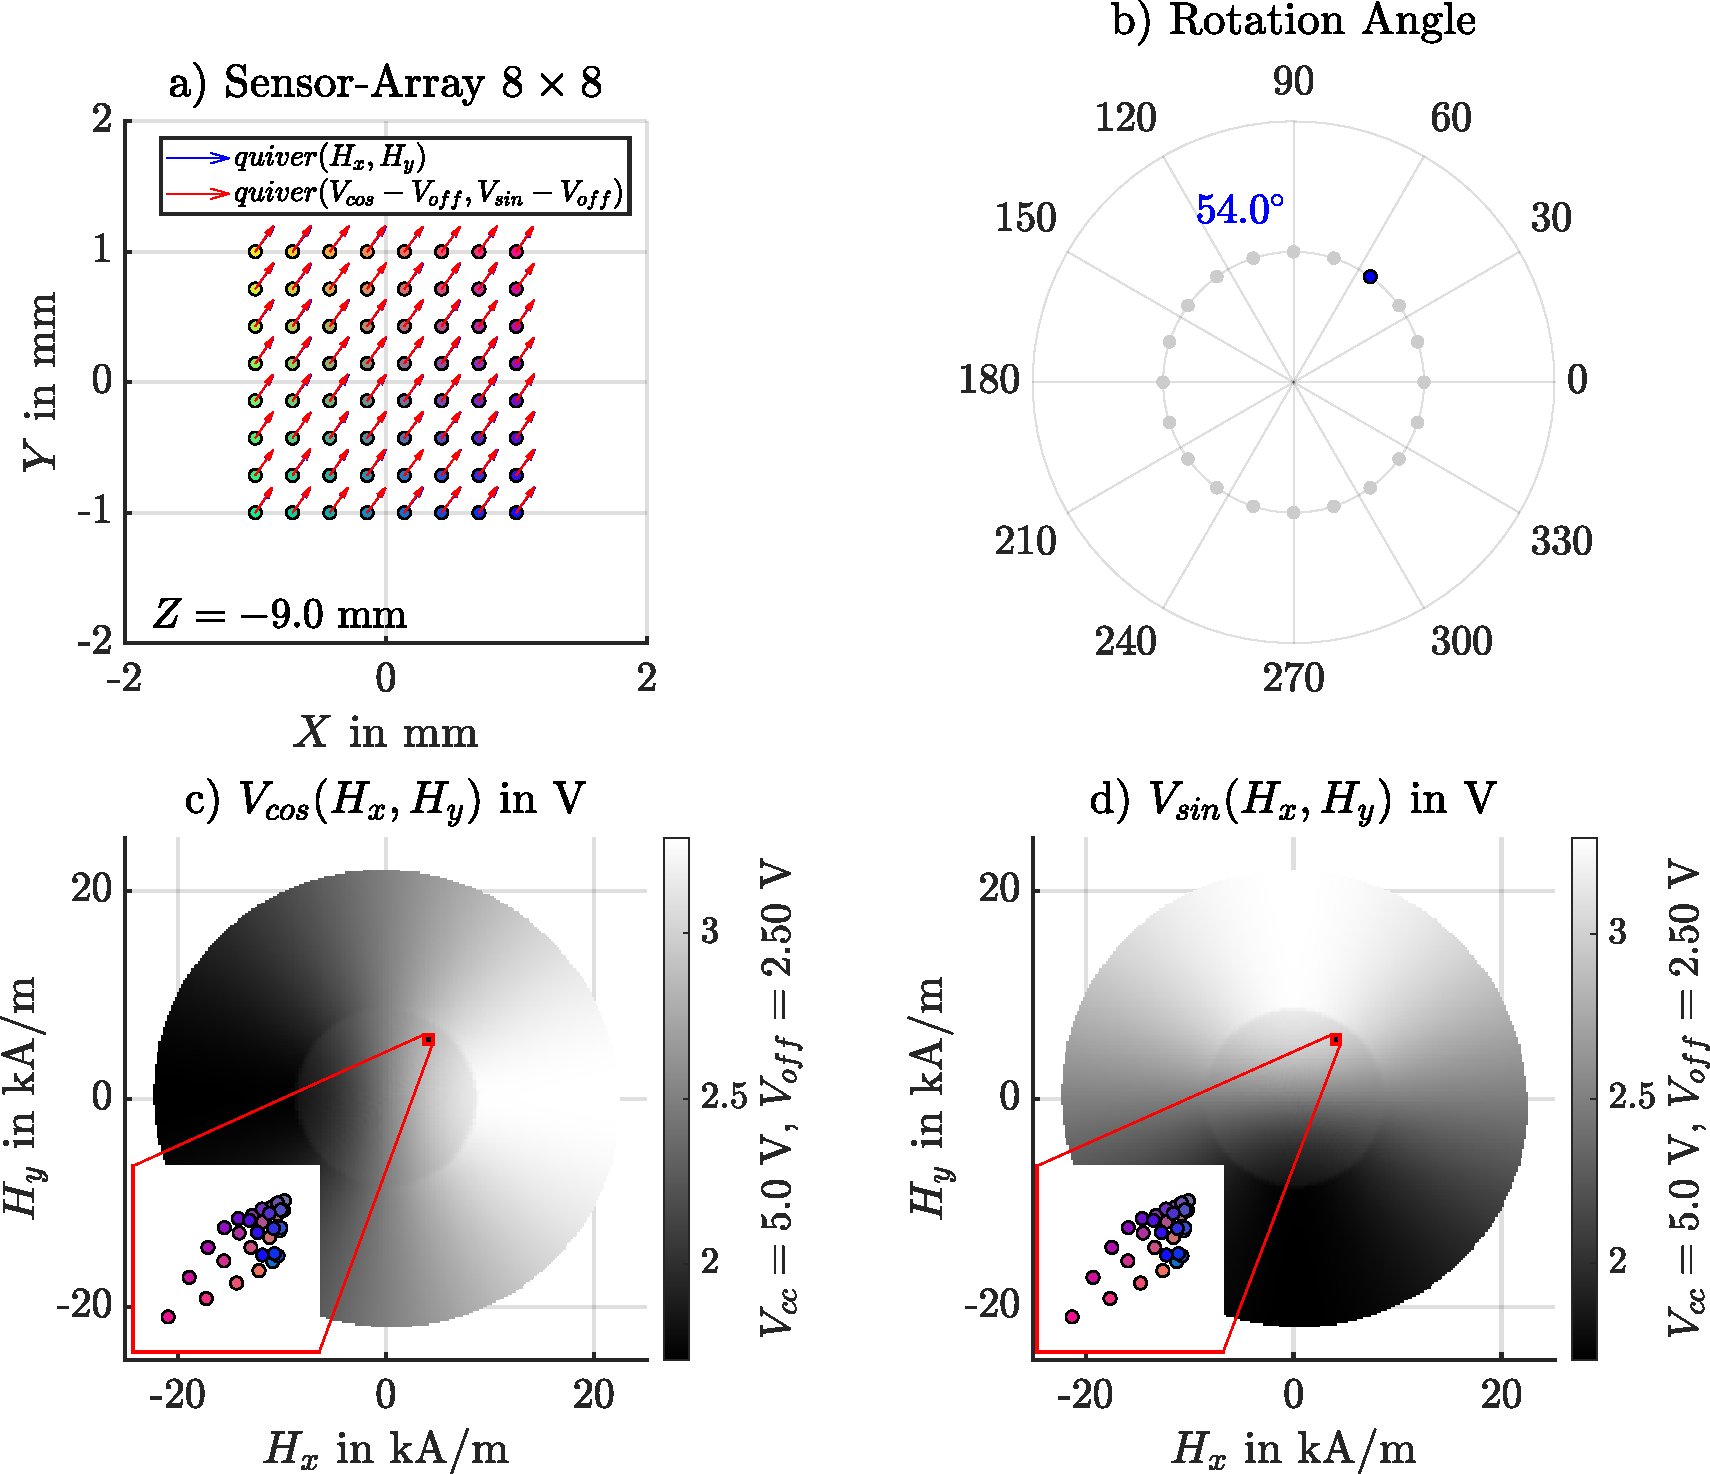
\includegraphics[width=.99\linewidth]{appendix/images/5-Sensor-Array-Sim-Imp/Kennfeld-Mapping}
	\caption[Kennfeld-Mapping]{Kennfeld-Mapping. Entnahme von Referenzspannungen aus den Sensor-Kennfeldern, gezeigt für einen beliebigen Simulationswinkel. In a) Meshgrid des Sensor-Arrays mit Grundposition $(0,0,-9)^T \SI{}{\milli\metre}$ relativ zum Koordinatenursprung (mag. Dipol). Simulation ohne Dipol-Verkippung. b) Simulation für $20$ gleich verteilte Winkel, gezeigt ist der vierte Winkel bei $\SI{54}{\degree}$. Simulationsparameter sind wie in \autoref{tab:sensor-array-sim-params} eingestellt. Magnet und Array-Position sind ideal konfiguriert. Ersichtlich anhand des eng gegliederten Feldstärken-Mappings auf c) Cosinus-Kennfeld und d) Sinus-Kennfeld. Die simulierten Feldstärken für alle Sensor-Pixel-Koordinaten, liegen innerhalb des linearen Kennfeldarbeitsbereich. Die Kennfelder sind entsprechend Betriebsspannungsparametrierung in $\SI{}{\volt}$ umgerechnet.}
	\label{fig:kennfeld-mapping}
\end{figure}


\clearpage


\autoref{fig:kennfeld-mapping} zeigt das Mapping auf TMR-Sensor-Kennfeldern (\autoref{ch:tdk-datensatz}) für prozessierte $H_x$- und $H_y$-Feldstärken. Die Simulation ist mit der Standardparametrierung aus \autoref{tab:sensor-array-sim-params} ausgeführt worden. Hier am Beispiel für $20$ Simulationswinkel. Gezeigt ist der vierte Winkel bei $\SI{54}{\degree}$. Die errechneten Feldstärken sind auf die Kennfelder projiziert und Spannungswerte mittels Matlab-2D-Interpolation für Nearest-Neighbor entnommen. \autoref{fig:senor-array-teilansicht} zeigt, das nochmal für $720$ Winkel und vier Sensor-Pixel. Es sind die Eck-Pixel angezeigt. Da sich der magnetische Dipol ohne Verkippung, zentriert über dem Sensor-Array befindet, überlagern sich die Signalverläufe für diagonal gegenüberliegende Sensor-Pixel. Der leicht ellipsenförmige Verlauf der projizierten Feldstärken der äußeren Pixel, ergibt sich durch den Versatz zur Magnetfeldmitte. Ein Pixel direkt lotrecht zur Magnet-$Z$-Achse platziert, erzeugt einen optimale Kreisbahn. Eine detaillierte Beschreibung des Funktionsmoduls ist in \autoref{mcode:sensorarraysimulation} einzusehen.


\vspace{4mm}
\begin{figure}[bph]
	\centering
	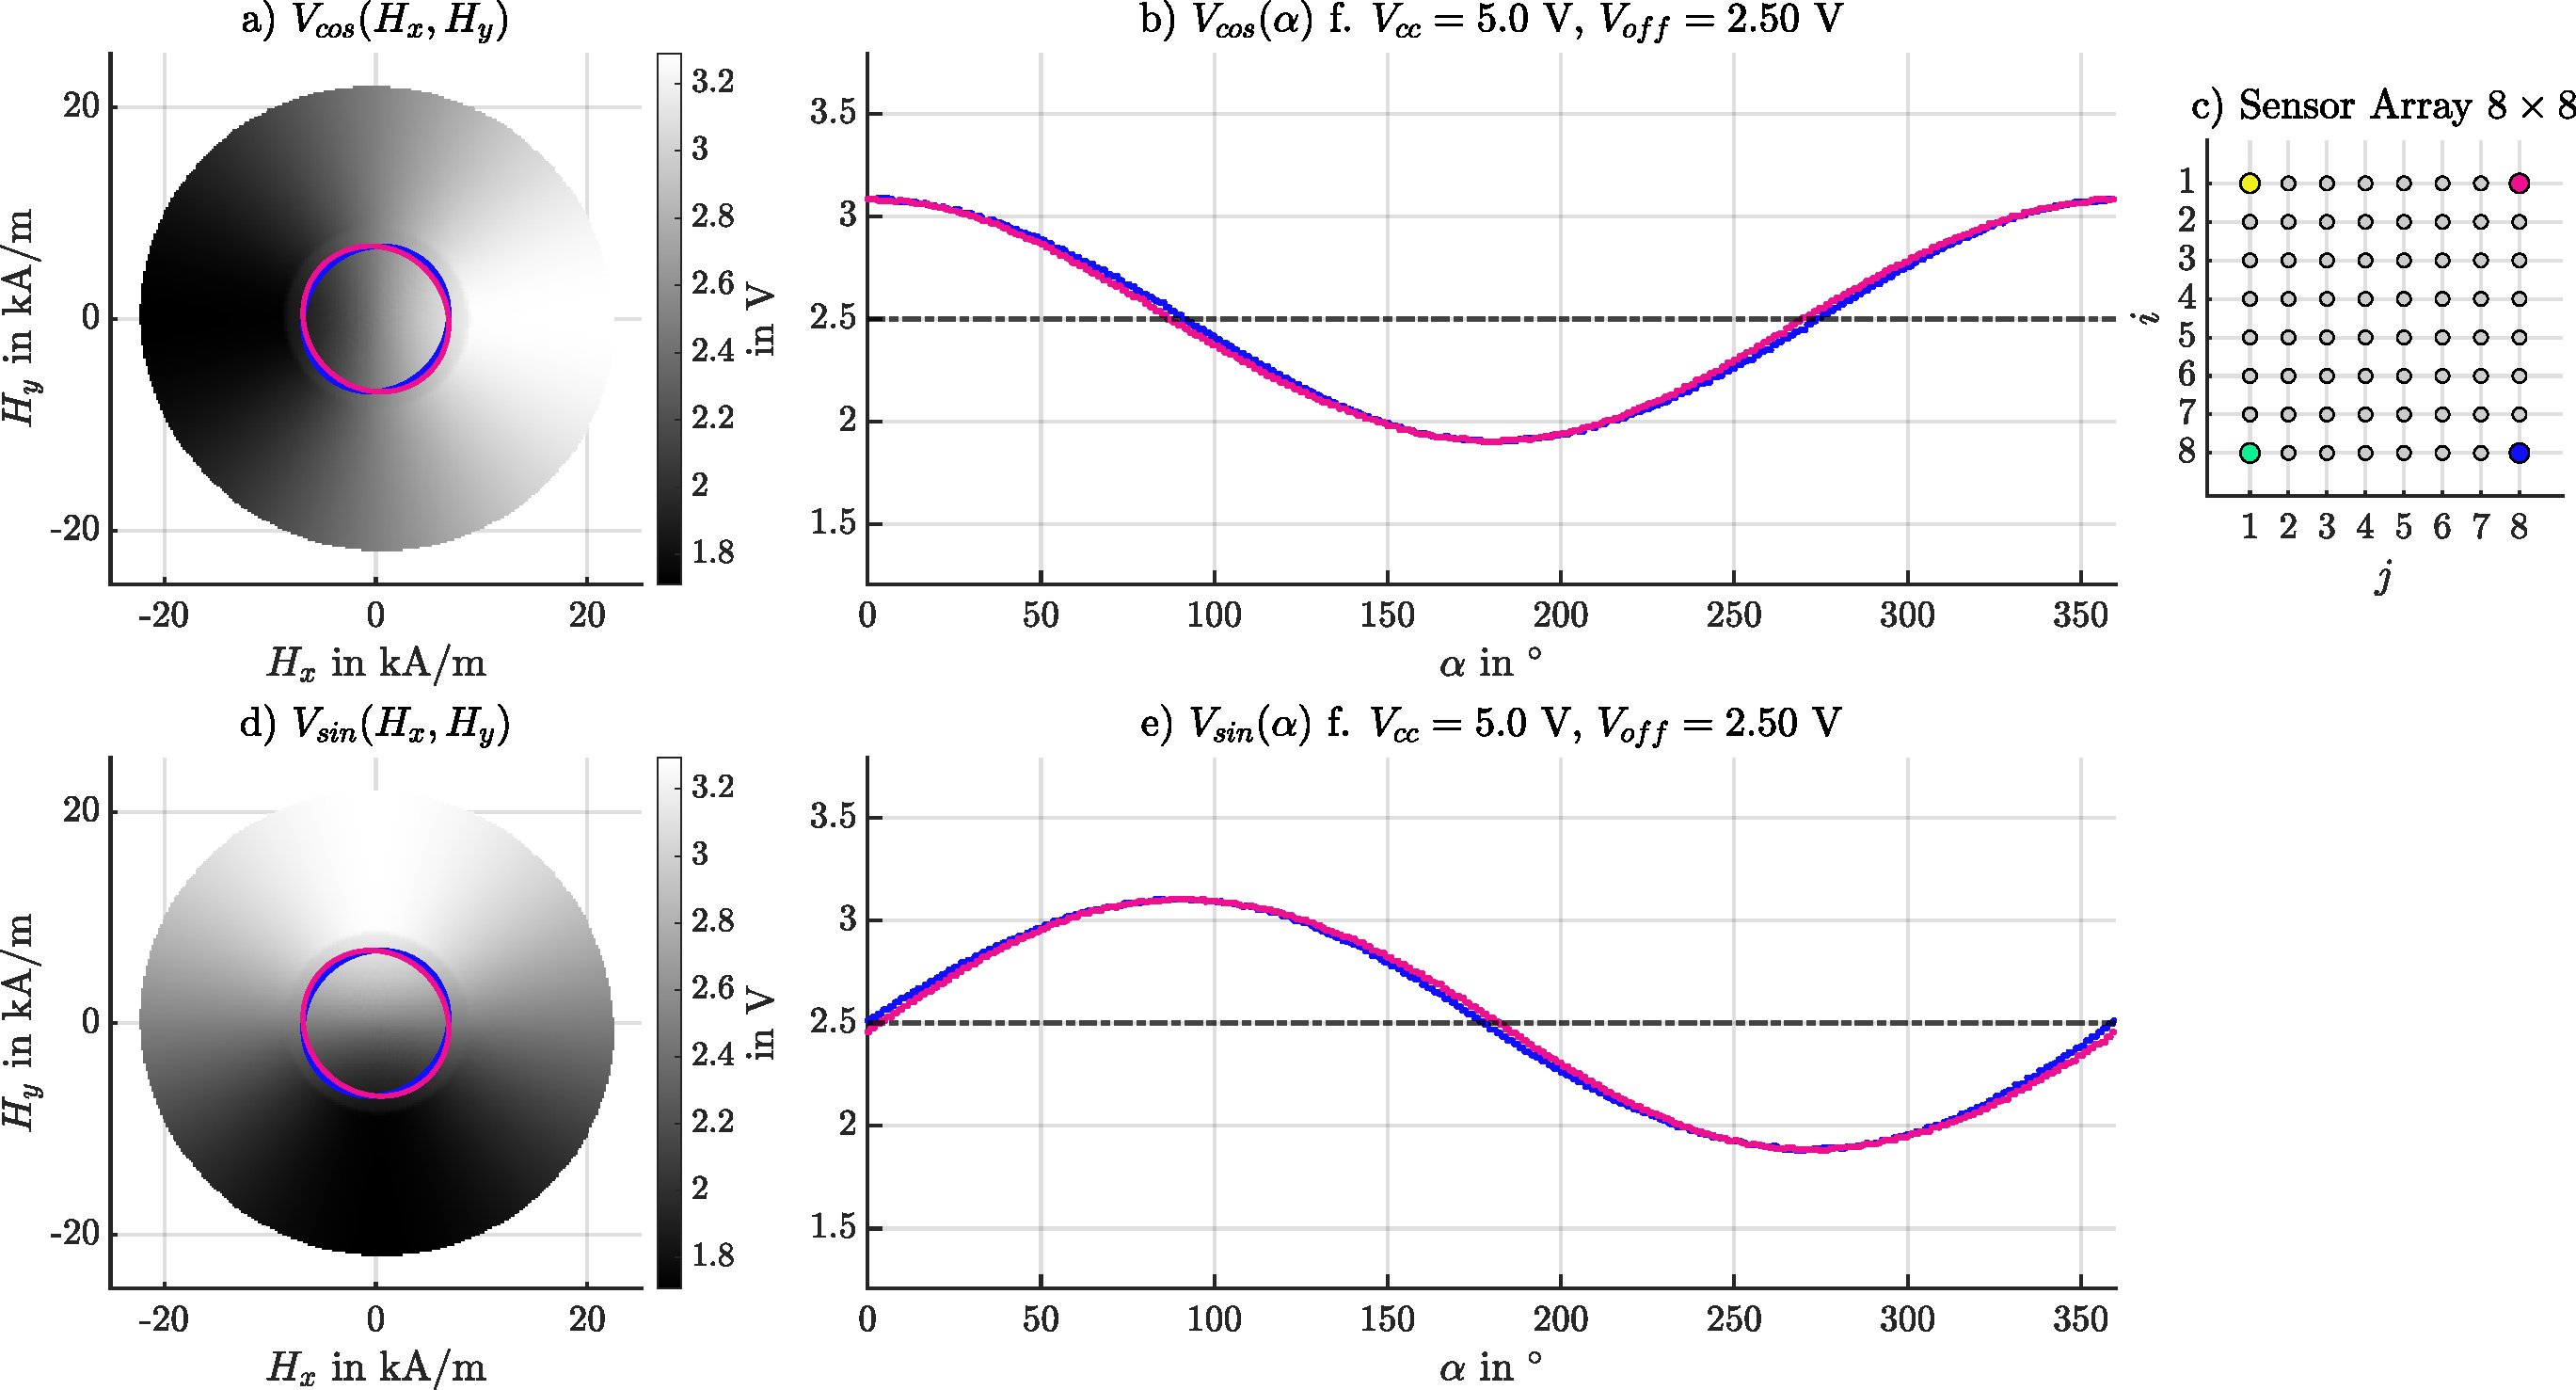
\includegraphics[width=\linewidth]{appendix/images/5-Sensor-Array-Sim-Imp/Senor-Array-Teilansicht}
	\caption[Sensor-Array-Datensatz, Teilansicht]{Sensor-Array-Datensatz, Teilansicht. Teilansicht der Simulationsergebnisse entsprechend der Parametrierung nach \autoref{tab:sensor-array-sim-params}. Es ist der gesamte Simulationsdurchlauf für die Eck-Sensor-Pixel c) gezeigt. a) und d) zeigen das Kennfeld-Mapping für korrespondierende Feldstärken bei einer vollständigen Dipol-Drehung. b) und e) stellen die Rotation aufgetragen über alle Simulationswinkel dar. Die sich diagonal gegenüberliegenden Sensor-Pixel überlagern sich in den Darstellungen a), b), d) und e). Das entspricht der Kreuzsymmetrieeigenschaft Dipol-Magnetfeldes. Das Sensor-Array ist zentriert zum Dipol ausgerichtet. Der Dipol ist nicht verkippt. Grafik nachempfunden aus \cite{Schuethe2019}}
	\label{fig:senor-array-teilansicht}
\end{figure}

% !TEX root = ../thesis.tex
% mathematical basic for GPR
% @author Tobias Wulf
%

\chapter{Gauß-Prozess-Regression Implementierung 0.0.1 13.04.2021}\label{ch:gpr-imp}


Im Anhang befindet sich die Beschreibung, der Regression mittels Gauß'scher Prozesse. Die implementierten Mechanismen sind auf die Sensor-Array-Simulation \autoref{ch:sensor-array-sim-imp} angepasst. Es wird sich  an der Anforderungsbeschreibung für ein TMR-Sensor-Array \autoref{sec:prinzip-des-sensor-arrays} orientiert. Eine Standardparametrierung für die Simulationsdurchführung ist in \autoref{tab:gpr-sim-params} einzusehen. Die Notation ist der kompakten Schreibweise für Gauß'sche Prozesse \cite{Rasmussen2006} angepasst. Implementiert ist ein Kernel aus den Vorarbeiten \cite{Schuethe2020b}\cite{Schuethe2020}. Darauf aufbauend ist ein zweiter mit angepasster Eingangswertverarbeitung entworfen worden. Beide Kernel besitzen die Fähigkeit zur Mittelwert freien und Polynom gestützten Regression bzw. Vorhersage \cite{Rasmussen2006}. Das Regressionsmodell kann ganze Sensor-Array-Datensätze verarbeiten. Es sind verschieden Qualitätskriterien implementiert, die Aussagen zur Modellgenauigkeit, Vorhersagesicherheit und Generalisierung treffen. Die Trainingsphase für das Regressionsmodell wird durch \autoref{alg:bayesopt} durchgeführt. Eine anschließende Arbeitsphase ist durch \autoref{alg:gprvorhersage} umgesetzt. Einen Überblick über die Gesamtsoftware, in der dieser Teil ein Modul einnimmt, ist im \autoref{mcode:gaussianprocessregression} einzusehen. Der Anhang besitzt einen Glossar ähnlichen Charakter und soll als Schnellnachschlagewerk unterstützen.


\vspace{4mm}
\begin{table}[!hbp]
	\centering
	\resizebox{\textwidth}{!}{
		\begin{tabular}{l l c c l}
			\toprule
			\textbf{Parametergruppe}     & \textbf{Parameter}  & \textbf{Wert}                        & \textbf{Einheit} & \textbf{Kurzbeschreibung}                                           \\ \midrule
			\multirow{10}{*}{GPROptions} & kernel              & 'QFCAPX'                             & char             & Kernel-Funktion-Indikator \eqref{eq:kfun}, 'QFC' $\leftarrow d_F^2$ \\
			                             & $\theta$            & $(1,1)$                              & -                & Kernel-Parametervektor $\theta$ \eqref{eq:kparam}                   \\
			                             & $\sigma_f^2$-Bounds & $(0.1, 100)$                         & -                & Parameter-Bounds $\theta_1$ f. \autoref{alg:fminconopt}             \\
			                             & $\sigma_l$-Bounds   & $(0.1, 100)$                         & -                & Parameter-Bounds $\theta_2$ f. \autoref{alg:fminconopt}             \\
			                             & $\sigma_n^2$        & $1 \cdot 10^{-6}$                    & -                & Rauschniveau, Rauschaufschaltung \eqref{eq:addnoise}                \\
			                             & $\sigma_n^2$-Bounds & $(1 \cdot 10^{-8}, 1 \cdot 10^{-4})$ & -                & Parameter-Bounds $\sigma_n^2$ f. \autoref{alg:bayesopt}             \\
			                             & OptimRuns           & $30$                                 & -                & Durchlaufanzahl f. \autoref{alg:bayesopt}                           \\
			                             & SLL                 & 'SLLA'                               & char             & Verlust-Indikator f. Winkel (A)/ R (Radius) \autoref{alg:bayesopt}  \\
			                             & mean                & 'zero'                               & char             & Indikator Mittelwertpolynom Ein ('poly')/ Aus ('zero')              \\
			                             & polyDegree          & $1$                                  & -                & Grad des Mittelwertpolynoms wenn mean = 'poly'                      \\ \bottomrule
		\end{tabular}}
	\caption[Gauß-Prozess-Regression-Simulationsparameter]{Gauß-Prozess-Regression-Simulationsparameter. Default-Parameter für die Prozessierung von Simulationsergebnissen aus der Sensor-Array-Simulation \autoref{ch:sensor-array-sim-imp}.}
	\label{tab:gpr-sim-params}
\end{table}


\clearpage



\section{Modellinitialisierung}\label{sec:gprinit}


Die Modellinitialisierung zur Gauß-Prozess-Regression erfolgt nach \autoref{alg:gprinit}. Dabei sind Modellparametrierung über einen Konfigurationsdatensatz \autoref{tab:gpr-sim-params} zu laden. Ebenfalls sind alle gewählten Trainingsdaten, mit dazugehörigen Simulationswinkel $X \mapsto \alpha_{Ref}$, in die Initialisierung einzuspeisen. Das Modell wird Schritt für Schritt in einem Struct aufgebaut. Dabei sind bestimmte Funktionalitäten, entsprechend der gewählten Konfigurierung, in Funktions-Handles zugewiesen. So sind die Schritte $2, 4, 5$ und $7$ als Funktions-Handles umgesetzt. Das verringert den Speicheraufwand und benötigte Rechenergebnis können dynamisch bei Bedarf erzeugt werden. Nach der Initialisierung müssen, Modellkonfiguration aus Schritt $1$, die Regressionsziele aus Schritt $3$, die $L$-Matrix aus Schritt $8$ und die Regressionsgewichte aus Schritt $12$ als gespeicherte Werte, für die Vorhersage nach \autoref{alg:gprvorhersage} vorliegen. Die Modellkonfiguration aus Schritt $1$ und die berechneten Modellplausibilitäten aus Schritt $13$ sind für die Modelloptimierung nach \autoref{alg:fminconopt} entscheidend. Das Modell wird in der Optimierung z.T. reinitialisiert. Die einzelnen Initialisierungsschritte sind nachfolgend zusammengefasst aufgeführt. Es ist ein mathematisch Bezug zur Implementierung in \autoref{ch:sw-doku} und Notation nach Fachliteratur \cite{Rasmussen2006} vorgenommen worden.


\begin{algorithm}[bhp]
	\SetAlgoLined
	\KwIn{Konfigurationsdatensatz, Trainingsdatensatz $X \mapsto \alpha_{Ref}$}
	\KwResult{Regressionsmodell mit Fähigkeit zur Datensatzverabeitung aus \autoref{ch:sensor-array-sim-imp}}
	\textbf{1.} Initialisierung Modellkonfiguration $\leftarrow$ \autoref{tab:gpr-sim-params}\;
	\textbf{2.} Initialisierung $X$, $\alpha$ und $X$-Formatierung $\leftarrow$ \autoref{eq:trainds}, \autoref{eq:testds}\;
	\textbf{3.} Initialisierung Regressionsziele $\leftarrow$ \autoref{eq:gprtarget}\;
	\textbf{4.} Initialisierung Kernel-Funktion $\leftarrow$ \autoref{eq:kfun}\;
	\textbf{5.} Initialisierung Basis-Funktion $\leftarrow$ \autoref{eq:hfun}\;
	\textbf{6.} Berechnung $K(X,X|\theta) \leftarrow$ \autoref{alg:kmatrix}\;
	\textbf{7.} Rauschaufschaltung $K_y \leftarrow$ \autoref{eq:addnoise}\;
	\textbf{8.} Cholesky-Zerlegung von $K_y$ zu $L$ u. Berechnung $\log |K_y|$ $\leftarrow$ \autoref{eq:chol}\;
	\textbf{9.} Initialisierung Mittelwertpolynome $\leftarrow$ \autoref{eq:hmatrix}\;
	\textbf{10.} Berechnung Polynomkoeffizienten $\leftarrow$ jeweils \autoref{alg:beta-koeffs} f. \autoref{eq:betacoeffs}\;
	\textbf{11.} Initialisierung Mittelwertfunktion $\leftarrow$ \autoref{eq:gprmean}\;
	\textbf{12.} Berechnung Regressionsgewichte $\leftarrow$ \autoref{eq:gprweights}\;
	\textbf{13.} Berechnung Modellplausibilität $\leftarrow$ \autoref{eq:likelihoods}\;
	\caption{Modellinitialisierung mit konst. Trainingsdaten und Parametern}
	\label{alg:gprinit}
\end{algorithm}


\clearpage


\paragraph*{Trainingsdatensatz} definiert nach der kompakten Notation aus \cite{Rasmussen2006}. Ein Trainingsdatensatz $X$ beinhaltet alle Referenzwinkelstellungen $\alpha_i$ mit $X_i \mapsto \alpha_i$, nach der Beschreibung in \autoref{sec:prinzip-des-sensor-arrays} mit $X_{cos,i} = A_x$ und $X_{sin,i} = A_y$. Für die Implementierung mit \autoref{eq:de2innorm} müssen alle Trainingsdatenmatrizen normiert sein, sodass sich Vektoren als Trainingsdaten abbilden, siehe \autoref{eq:trainds}.


\begin{align}\label{eq:trainds}
	X   &= \big[ X_i, \ldots X_{N_{Ref}} \big] \qquad\qquad\qquad\quad\!  \text{f. } i = 1,2,3,\ldots,N_{Ref} \nonumber \\
	\\
	X_i &= 
		\begin{cases}
			\big[ X_{cos,i}, X_{sin,i} \big]             &\qquad \text{f. } d_F^2 \text{ \eqref{eq:df2}} \\
			\big[ \|X_{cos,i}\|_F, \|X_{sin,i}\|_F \big] &\qquad \text{f. } d_E^2 \text{ \eqref{eq:de2innorm}}
		\end{cases} \nonumber \\
	X_i & \mapsto \alpha_i \nonumber
\end{align}


\paragraph*{Testdatensatz} definiert in kompakter Schreibweise nach \cite{Rasmussen2006}. Ein Testdatensatz $X_*$ repräsentiert einen Testwinkel mit $X_* \mapsto \alpha_*$. Auch hier gilt, wie für Trainingsdatensätze $X_i \mapsto \alpha_i$, die Umschreibung nach \autoref{sec:prinzip-des-sensor-arrays} mit $X_{cos*} = A_x$ und $X_{sin*} = A_y$. Jeweils für die gewählte Implementierung ist auch hier eine Eingangsverarbeitung der Datensätze notwendig \autoref{eq:testds}, sodass die Implementierung nach \autoref{eq:de2innorm} mit Skalaren statt Matrizen arbeitet. 


\begin{align}\label{eq:testds}
	X_* &= 
	\begin{cases}
		\big[ X_{cos*}, X_{sin*} \big]             &\qquad \text{f. } d_F^2 \text{ \eqref{eq:df2}} \\
		\big[ \|X_{cos*}\|_F, \|X_{sin*}\|_F \big] &\qquad \text{f. } d_E^2 \text{ \eqref{eq:de2innorm}}
	\end{cases} \\
	X_* & \mapsto \alpha_* \nonumber
\end{align}


\clearpage


\paragraph*{Regressionsziele} sind als Spaltenvektoren nach \cite{Rasmussen2006} wie in \autoref{eq:gprtarget} definiert. Die Besonderheit hier sind zwei Zielvektoren statt einer, wie in der Fachliteratur \cite{Rasmussen2006} angegeben. Abstrahiertes Regressionsziel ist der Einheitskreis, daher ergeben sich einfache Sinoide aus den Referenzwinkeln in \autoref{eq:gprtarget}.


\begin{align}\label{eq:gprtarget}
	y_{cos} &= (\cos \alpha_i, \ldots, \cos \alpha_{N_{Ref}})^T \qquad \text{f. } i = 1,2,3,\ldots,N_{Ref} \nonumber \\
	\\
	y_{sin} &= (\sin \alpha_i, \ldots, \sin \alpha_{N_{Ref}})^T \nonumber
\end{align}


\paragraph*{Kernel-Funktion} als Kernelement des Regressionsverfahren für Gauß'sche Prozesse \cite{Rasmussen2006}. Es sind zwei Versionen nach gleichen Vorbild der fraktalen Kovarianz \cite{Schuethe2020b}\cite{Schuethe2020}  implementiert. Die Implementierung mittels \autoref{eq:df2} resultiert aus den Vorarbeiten der \gls{gl:ags} und stellt die genaue Lösung dar und arbeitet direkt mit Matrizen als Trainingsdaten. Die Implementierung nach mit \autoref{eq:de2innorm} ist innerhalb dieser Arbeit entstanden und bedingt ein vorab Prozessieren der Trainingsdaten zu Vektoren. Ebenfalls müssen weitere Testdaten eingangs zu skalaren verarbeitet werden. Dazu wird die Frobenius-Norm aus \autoref{eq:fnorm} verwendet. Die Implementierung nach \autoref{eq:de2innorm} folgt dem Beispiel, aus einer Veröffentlichung der TU-München \cite{Lang2014}, für die Anwendung der Gauß-Prozess-Regression auf Themenfeld der Robotik.


\begin{align}\label{eq:kfun}
	k(X_i, X_j) &= 
		\begin{cases}
			\resizebox{.17\linewidth}{!}{$\frac{a}{b + d_F^2\langle X_i, X_j \rangle}$} &\qquad \text{f. } d_F^2 \text{ \eqref{eq:df2}} \\\\
			\resizebox{.17\linewidth}{!}{$\frac{a}{b + d_E^2\langle X_i, X_j \rangle}$} &\qquad \text{f. } d_E^2 \text{ \eqref{eq:de2innorm}}
		\end{cases} \\
\text{mit } i,j &= 1,2,3,\ldots,N_{Ref} \nonumber
\end{align}


\clearpage


\paragraph*{Kernel-Parameter} für die Kovarianz- oder Kernel-Funktion bilden sich die Funktionsparameter, wie in \autoref{eq:kparam} beschrieben. Bei der Parameteridentifizierung ist das Auslöschungskriterium für gültige Kovarianzfunktionen elementar \cite{Rasmussen2006}. Dabei ist der Fall abzudecken, dass die Abstandsfunktion der Kovarianz zu null wird, wenn Datensätze mit sich selbst prozessiert werden. In diesem Fall muss die Kovarianzfunktion $\sigma_f^2$ ergeben.


\begin{equation}\label{eq:kparam}
	a = \sigma_f^2 \cdot 2 \sigma_l^2 \qquad b = 2 \sigma_l^2 \qquad \theta = \left[\sigma_f^2, \sigma_l\right]
\end{equation}


\paragraph*{Kovarianzmatrix} als Autokorrelationsergebnis, ist für alle bereitgestellten Trainingsdaten untereinander mit \autoref{alg:kmatrix} zu berechnen \cite{Rasmussen2006}. Das Ergebnis, in quadratischer Matrixform, definiert das Verhalten des Gesamtsystems über gemessene Einzelabstände der Trainingsdaten zueinander. Es bedeutet, dass für ein Sensor-Array auf Basis des TMR-Sensors \cite{TDK2016} in Drehwinkelapplikation \autoref{fig:sensor-array-prinzip}, die $\SI{360}{\degree}$ Periodizität ersichtlich sein muss. Was eine Maxima-Diagonale von links nach rechts und annähernde Max-Werte in den beiden übrigen Ecken der Matrix impliziert.


\begin{algorithm}[h]
	\SetAlgoLined
	\KwIn{Kernel-Funktion $k(X_i, X_j)$, Trainingsdaten $X$, Kernel-Parameter $\theta$}
	\KwResult{$K$-Matrix $N_{Ref} \times N_{Ref}$ }
	\textbf{1.} Initialisierung Parameter $(a,b) \leftarrow \theta$ \autoref{eq:kparam}\;
	\textbf{2.} \For{$i=1,2,3,\ldots,N_{Ref}$}{
		\For{$j=1,2,3,\ldots,N_{Ref}$}{
			$K_{i,j} = k(X_i, X_j) \leftarrow$ \autoref{eq:kfun}\; 
		}
	}
	\caption{Berechnung der Kovarianzmatrix $K(X, X|\theta)$}
	\label{alg:kmatrix}
\end{algorithm}


\paragraph*{Rauschaufschaltung} durch konstantes Rauschniveau $\sigma_n^2$ und minimaler Anhebung der Kovarianzmatrix-Diagonalen, für verrauschte bzw. fehlerbehaftete Regression \cite{Rasmussen2006}. Entsprechend der Fachliteratur ist die Kovarianzmatrix inklusive additives Rauschen als $K_y$ bezeichnet \cite{Rasmussen2006}.


\begin{equation}\label{eq:addnoise}
	K_y = K(X, X|\theta) + \sigma_n^2 I
\end{equation}


\paragraph*{Cholesky-Zerlegung $K_y$} als Ansatz zum Lösen der Regressionsmechanismen. Dem Regressionsverfahren zugrundeliegenden Lösungen der Wahrscheinlichkeitsdichte-Integrale sind über Matrix- und Vektormultiplikation mit Inversen Matrizen in linearen Gleichungssystemen gelöst \cite{Rasmussen2006}. Für das Lösen der Gleichungssysteme mit inversen Matrizen, ist die Zerlegung der nicht inversen Matrix in eine untere Dreiecksmatrix möglich. Die Cholesky-Zerlegung schafft entsprechenden Repräsentant $L$ für die Matrix $K_y$. Die logarithmierte Determinante ist mit \autoref{eq:chol} zu berechnen. Matrizen müssen symmetrisch und positiv definit sein, um die Cholesky-Zerlegung anwenden zu können \cite{Rasmussen2006}.


\begin{align}\label{eq:chol}
		 LL^T &= K_y  \nonumber \\
		 \\
	log |K_y| &= 2 \sum_{i=1}^{N_{Ref}} \log L_{i,i} \nonumber
\end{align}


Es sollen damit Gleichungssysteme wie $Ax = b \Leftrightarrow x = A^{-1}b$ über zerlegten Repräsentanten gelöst sein $Ly = b \Leftrightarrow L^Tx = y$. Als Notation für die notwendige Lösung der linearen Gleichungssystem ist der Backslash-Operator genutzt $x = L^T \backslash (L \backslash b)$ \cite{Rasmussen2006}. Der Backslash-Operator steht ebenfalls in Matlab zur Verfügung.


\paragraph*{Basis-Funktion} als Aufbaufunktion für Polynome aus Trainings- und Testdaten. Das Regressionsverfahren mittels Gauß'scher Prozesse kann in zwei Ausführungen betrieben werden. Die erste ist eine Regression ohne weitere Mittelwerte als Regressionshilfe. In zweiter Ausführung können Mittelwerte der Daten z.B. über Polynomfindung gebildet sein. Dafür bedingt es eine Basis-Funktion nach \autoref{eq:hfun}, die entsprechend der Kernel-Funktion und resultierende Datenformate Polynome bildet \cite{Rasmussen2006}. In der Implementierung sind Polynome ersten Grades verwendet. Was einer Offset- und Amplitudenkorrektur der Trainings- und Testdaten entspricht. Die in \autoref{eq:hfun} gezeigten Funktionen müssen, jeweils für beide Cosinus und Sinus Datentypen gebildet werden und beziehen sich hier in der Darstellung für einen einzigen Simulationswinkel $X_* \mapsto \alpha_*$.


\begin{align}\label{eq:hfun}
	h_{cos}(X_{cos*}) &=
		\begin{cases}
			0								                          & \text{f. } m_{cos}(X_{cos*}) = 0 \\
			\big( 1, \|X_{cos*}\|_F, \|X_{cos*}\|_F^2, \ldots \big)^T & \text{f. } d_F^2 \text{ \eqref{eq:df2}, }       m_{cos}(X_{cos*}) \ne 0 \\
			\big( 1, X_{cos*}, X_{cos*}^2, \ldots \big)^T             & \text{f. } d_E^2 \text{ \eqref{eq:de2innorm}, } m_{cos}(X_{cos*}) \ne 0
		\end{cases} \nonumber \\
	\\
	h_{sin}(X_{sin*}) &=
		\begin{cases}
			0								                          & \text{f. } m_{sin}(X_{sin*}) = 0 \\
			\big( 1, \|X_{sin*}\|_F, \|X_{sin*}\|_F^2, \ldots \big)^T & \text{f. } d_F^2 \text{ \eqref{eq:df2}, }       m_{sin}(X_{sin*}) \ne 0 \\
			\big( 1, X_{sin*}, X_{sin*}^2, \ldots \big)^T             & \text{f. } d_E^2 \text{ \eqref{eq:de2innorm}, } m_{sin}(X_{sin*}) \ne 0
		\end{cases} \nonumber
\end{align}


\paragraph*{Mittelwertpolynome} bauen sich über die Basis-Funktionen aus \autoref{eq:hfun} für Trainingsdaten auf. Es resultieren Matrizen \cite{Rasmussen2006}, deren erste Reihe gleich eins ist und jede weitere Reihe mit entsprechenden Exponent für die Polynomgenerierung versehen ist. Die Polynombildung ist jeweils für beide Cosinus- und Sinus-Datensätze durchzuführen, wenn die Mittelwertbildung aktiv ist.


\begin{align}\label{eq:hmatrix}
	H_{cos}(X_{cos}) &=
		\begin{cases}
			0 															   &\qquad \text{f. } m_{cos}(X_{cos}) = 0 \\
			\big[ h_{cos}(X_{cos,i}),\ldots,h_{cos}(X_{cos,N_{Ref}}) \big] &\qquad \text{f. } m_{cos}(X_{cos}) \ne 0
		\end{cases} \nonumber \\
	\\
	H_{sin}(X_{sin}) &=
		\begin{cases}
			0															   &\qquad \text{f. } m_{sin}(X_{sin}) = 0 \\
			\big[ h_{sin}(X_{sin,i}),\ldots,h_{sin}(X_{sin,N_{Ref}}) \big] &\qquad \text{f. } m_{sin}(X_{sin}) \ne 0
		\end{cases} \nonumber \\
	\nonumber \\
	& \text{jeweils für alle } X_{cos} = \big[ X_{cos,i},\dots, X_{cos,N_{Ref}} \big] \text{ und } \nonumber \\
	& \text{alle } X_{sin} = \big[ X_{sin,i},\dots, X_{sin,N_{Ref}} \big] \nonumber \\
	& \text{mit } i = 1,2,3,\ldots,N_{Ref} \nonumber
\end{align}



\paragraph*{Polynomkoeffizienten} zur Mittelwertbildung über gebildet Polynome nach \autoref{eq:hfun} und \autoref{eq:hmatrix}, sind benötigte Polynomkoeffizienten nach \autoref{eq:betacoeffs} zu berechnen \cite{Rasmussen2006}. Zur Berechnung der Koeffizienten sind mehrere inverse Matrix-Produkte verschachtelt zu lösen. 


\clearpage


\begin{align}\label{eq:betacoeffs}
	\beta_{cos} &= 
		\begin{cases}
			0 																	 &\qquad \text{f. } m_{cos}(X_{cos}) = 0\\
			\big( H_{cos} K_y^{-1} H_{cos}^T \big)^{-1} H_{cos} K_y^{-1} y_{cos} &\qquad \text{f. } m_{cos}(X_{cos}) \ne 0
		\end{cases} \nonumber \\
	\\
	\beta_{sin} &= 
		\begin{cases}
			0 																	 &\qquad \text{f. } m_{sin}(X_{sin}) = 0\\
			\big( H_{sin} K_y^{-1} H_{sin}^T \big)^{-1} H_{sin} K_y^{-1} y_{sin} &\qquad \text{f. } m_{sin}(X_{sin}) \ne 0
		\end{cases} \nonumber \\
	\nonumber \\
	& \text{jeweils für alle } X_{cos} = \big[ X_{cos,i},\dots, X_{cos,N_{Ref}} \big] \text{ und } \nonumber \\
	& \text{alle } X_{sin} = \big[ X_{sin,i},\dots, X_{sin,N_{Ref}} \big] \nonumber \\
	& \text{mit } i = 1,2,3,\ldots,N_{Ref} \nonumber
\end{align}


Zur Bewältigung des Problems ist \autoref{alg:beta-koeffs} implementiert worden und jeweils für beide Cosinus- und Sinus-Polynome aus \autoref{eq:hmatrix} durchzuführen. Die Polynom- und Koeffizientenbestimmung entfällt, wenn die Mittelwertbildung ausgeschaltet ist.


\begin{algorithm}[hp]
	\SetAlgoLined
	\KwIn{Polynommatrix $H$, Untere Dreiecksmatrix $L(K_y)$, Regressionsziel $y$}
	\KwResult{$\beta$-Koeffizienten}
	\textbf{1.} $a_0 \leftarrow$ Lösen von $K_y^{-1} y$\;
	\Indp 
		$a_0 = L^T \backslash (L \backslash y)$\;
	\Indm
	\textbf{2.} $A_1 \leftarrow$ Lösen von $H K_y^{-1} H^T$\;
	\Indp
		\For{j-te Spalte in $H^T$}{
			$V_j = L \backslash H_j^T$\;
		}
		$A_1 = V^T V$\;
	\Indm
	\textbf{3.} $L_1 \leftarrow$ $\text{cholesky}(A_1)$\;
	\textbf{4.} $A_2 \leftarrow$ Lösen von $A_1^{-1} H$\;
	\Indp
		\For{$j-te$ Spalte in $H$}{
			$V_j = L_1^T \backslash (L_1 \backslash H_j)$\;
		}
		$A_2 = V$\;
	\Indm
	\textbf{5.} $\beta = A_2 \cdot a_0$\;
	\caption{Berechnung der $\beta$ Polynomkoeffizienten aus \autoref{eq:betacoeffs}}
	\label{alg:beta-koeffs}
\end{algorithm}


\clearpage


\paragraph*{Mittelwertfunktionen} für die Regression setzen sich aus gebildeten Polynomen und den bestimmten Polynomkoeffizienten nach \autoref{eq:gprmean} zusammen \cite{Rasmussen2006}. Für alle Trainingsdaten mittels Polynommatrizen und für einzelne Testdaten über die Basis-Funktion. Bei eingeschalteter Mittelwertbildung, bildet sich das Regressionsergebnis über die Summe aus Mittelwertberechnung und Stützwertsumme \cite{Rasmussen2006}. Die Mittelwertrechnung ist für beide Cosinus- und Sinus-Datensätze umzusetzen. 


\begin{align}\label{eq:gprmean}
	m_{cos}(X_{cos(*)}) &=
		\begin{cases}
			0                                    &\qquad \text{f. mittelwertfreie Regression} \\
			H_{cos}(X_{cos}) \cdot \beta_{cos} 	 &\qquad \text{f. Trainingsdaten } X_{cos} \\
			h_{cos}(X_{cos*}) \cdot \beta_{cos} &\qquad \text{f. Testdaten } X_{cos*}
		\end{cases} \nonumber \\
	\\
	m_{sin}(X_{sin(*)}) &=
		\begin{cases}
			0                                    &\qquad \text{f. mittelwertfreie Regression} \\
			H_{sin}(X_{sin}) \cdot \beta_{sin} 	 &\qquad \text{f. Trainingsdaten } X_{sin} \\
			h_{cos}(X_{sin*}) \cdot \beta_{sin} &\qquad \text{f. Testdaten } X_{sin*}
		\end{cases} \nonumber \\
	\nonumber \\
& \text{jeweils für alle } X_{cos} = \big[ X_{cos,i},\dots, X_{cos,N_{Ref}} \big] \text{ und } \nonumber \\
& \text{alle } X_{sin} = \big[ X_{sin,i},\dots, X_{sin,N_{Ref}} \big] \nonumber \\
& \text{mit } i = 1,2,3,\ldots,N_{Ref} \nonumber
\end{align}


\clearpage


\paragraph*{Regressionsgewichte} oder Stützwerte für die Vorhersage beider Sinoide sind jeweils, in Abhängigkeit der dazugehörigen Regressionsziele und Mittelwerte, über inverse Matrix-Produkt aus $K_y^{-1}$ und das Residual aus Ziel und Mittelwert zu bilden. \autoref{eq:gprweights} beschreibt die Lösung des resultierenden Gleichungssystem über die untere Dreiecksmatrix $L$ der Kovarianzmatrix $K_y$ \cite{Rasmussen2006}. Die Gewichtsbildung veranschaulicht am besten den Gesamtablauf des Verfahrens. Es sind zwei unterschiedliche Regressionen, jeweils für Cosinus- und Sinus-Funktionen durchzuführen. Dabei stützen sich beide Regressionen auf eine gemeinsame Kovarianzbewertung, der zugrundeliegenden Trainingsdatensätze \cite{Schuethe2020}. Die Kovarianzmatrix stellt somit die vektorielle und orthogonale Kopplung der Daten her und impliziert ihre gegenseitige Abhängigkeit.


\begin{align}\label{eq:gprweights}
	\alpha_{cos} &= K_y^{-1} \cdot \big( y_{cos} - m_{cos}(X_{cos}) \big) \nonumber \\
				 &= L^T \backslash \Big(L \backslash \big( y_{cos} - m_{cos}(X_{cos}) \big) \Big) \nonumber \\
	\\
	\alpha_{sin} &= K_y^{-1} \cdot \big( y_{sin} - m_{sin}(X_{sin}) \big) \nonumber \\
				 &= L^T \backslash \Big(L \backslash \big( y_{sin} - m_{sin}(X_{cos}) \big) \Big) \nonumber \\
	\nonumber \\
& \text{jeweils für alle } X_{cos} = \big[ X_{cos,i},\dots, X_{cos,N_{Ref}} \big] \text{ und } \nonumber \\
& \text{alle } X_{sin} = \big[ X_{sin,i},\dots, X_{sin,N_{Ref}} \big] \nonumber \\
& \text{mit } i = 1,2,3,\ldots,N_{Ref} \nonumber
\end{align}


\clearpage


\paragraph*{Modellplausibilitäten} oder Regressionsevidenzen, sind entsprechend der Regressionsausrichtung, über Residuale und Regressionsgewichte in \autoref{eq:likelihoods} zu bilden \cite{Rasmussen2006}. Jeweils wieder für beide Cosinus- und Sinus-Datensätze. Die so aufgestellten Plausibilitäten bewerten den Regressions-Fit in Bezug auf die Trainingsdaten. In der Fachliteratur \cite{Rasmussen2006} sind diese auch als Logarithmic-Marginal-Likelihoods bezeichnet. Sie bieten einen Indikator für den Daten-Fit, der $< 0$ wird für eine schlechte Anpassung, $\approx 0$ ist bei mäßiger Anpassung und $> 0$ ist für eine gute Modellanpassung. Dabei sind Werte $> 30$ als sehr gute Anpassung Modellanpassung für jeweilige Sinoide zu interpretieren. Bei Plausibilitäten größer $> 60$ und zu eng gewählter Parameter-Bounds, kann sich ein zu Starker Fit auf die Trainingsdaten einstellen. Das wird als Overfitting bezeichnet. Ein so über parametriertes Modell, verliert dabei seine Fähigkeit zur Generalisierung und liefert nur für die Trainingsdaten selber valide Ergebnisse. Testdaten, die von den Trainingsdaten abweichen, können somit nicht mehr korrekt prozessiert werden. Die Interpretation der Likelihoods ist aus der Fachliteratur \cite{Rasmussen2006} entnommen und für empfohlene Werte empirisch bestimmt worden. Die einzelnen Plausibilitäten müssen ungefähr gleich groß sein, andernfalls besteht ein Ungleichgewicht in der Vorhersage. Resultierende Ergebnisse sind dann im Winkel und Radius verfälscht. Hergestellt wird das Gleichgewicht durch die Kovarianzkopplung, mittels gemeinsamer Kovarianzmatrix.


\begin{align}\label{eq:likelihoods}
	\log p(y_{cos}|X_{cos}) &= -0,5 \Big( \big( y_{cos} - m_{cos}(X_{cos}) \big)^T \alpha_{cos} + \log|K_y| + N_{Ref} \log 2\pi  \Big) \nonumber \\
	\\
	\log p(y_{sin}|X_{sin}) &= -0,5 \Big( \big( y_{sin} - m_{sin}(X_{sin}) \big)^T \alpha_{sin} + \log|K_y| + N_{Ref} \log 2\pi  \Big) \nonumber \\
	\nonumber \\
& \text{jeweils für alle } X_{cos} = \big[ X_{cos,i},\dots, X_{cos,N_{Ref}} \big] \text{ und } \nonumber \\
& \text{alle } X_{sin} = \big[ X_{sin,i},\dots, X_{sin,N_{Ref}} \big] \nonumber \\
& \text{mit } i = 1,2,3,\ldots,N_{Ref} \nonumber	
\end{align}


\clearpage


\section{Modelloptimierung}\label{sec:gpropt}


Die Optimierung bezieht sich auf ein fertig initialisiertes Modell nach \autoref{alg:gprinit}. Dieses muss dafür einen vollständigen Parametersatz \autoref{tab:gpr-sim-params} inklusive Bounds beinhalten. Ebenfalls müssen alle Trainingsdaten entsprechend der gewählten Implementierung im Modell enthalten sein. Die Optimierung in \autoref{alg:fminconopt} ist mittels Fmincon-Funktion (Matlab) implementiert und nutzt einen Sequential-Quadratic-Programming-Algorithmus um das Minimum-Kriterium aus \autoref{eq:fmincon} zu steuern. Das Modell wird im Prozess so lange reinitialisiert, bis keine graduelle Änderung des Kriteriums mehr festgestellt werden können. Kritisch im Optimierungsverfahren sind dabei, die zu setzenden Parameter-Bounds für $\theta$. Sind die Grenzen des Suchfeldes zu eng gesetzt, kann das Minimum nicht erreicht werden. Der Algorithmus wird dann die Bounds selbst als Ergebnis liefern. Sind die Bounds zu weit abgesteckt ist es theoretisch möglich, dass das Minimum nicht vor Abbruch gefunden werden kann. In der Regel findet sich das Minimum, mit der getroffenen Implementierung, nach $6-24$ Durchläufe. Das ist empirisch durch ausgegebene Grafiken beobachtet worden.


\begin{algorithm}[htp]
	\SetAlgoLined
	\KwIn{Modell inkl. $X$, $\theta,\sigma_n^2$ $+$ Bounds $\leftarrow$ \autoref{alg:gprinit}}
	\KwResult{Optimiertes Modell mit neuen Kernel-Parameter $\theta|\sigma_n^2$, f. $\sigma_n^2 = konst.$}
	\textbf{1.} Initialisierung Fmincon-Funktion\;
	\textbf{2.} Initialisierung Parameter-Bounds $\leftarrow$ Modell-Bounds \autoref{tab:gpr-sim-params}\;
	\textbf{3.} Initialisierung Fmincon-Startwert $\leftarrow$ Model-Kernel-Parameter \autoref{tab:gpr-sim-params}\;
	\textbf{4.} Initialisierung Min-Kriterium $\tilde{R}_{\mathcal{L}} \leftarrow$ \autoref{eq:fmincon}\;
	\textbf{5.} \While{$\neg(\tilde{R}_{\mathcal{L}} = konst.$ f. $7$ Iterationen$) \wedge (\min \ne \tilde{R}_{\mathcal{L}})$}{
		Zuweisung innerhalb Parameter-Bounds $\theta \leftarrow$ Fmincon-Funktion\;
		Modell-Teilreinitialisierung $\leftarrow$ \autoref{alg:gprinit}, Schritte 6. bis 13.\;
		Berechung $\tilde{R}_{\mathcal{L}} \leftarrow$ \autoref{eq:fmincon}\;
	}
	\textbf{6.} Speichern $\theta \leftarrow$ Fmincon-Funktion\;
	\textbf{7.} Modell-Teilreinitialisierung $\leftarrow$ \autoref{alg:gprinit}, Schritte 6. bis 13.\;
	\caption{Modelloptimierung über Fmincon-Funktion f. $\sigma_n^2 = konst.$}
	\label{alg:fminconopt}
\end{algorithm}


\clearpage


\paragraph*{Min-Kriterium} als zusammengesetztes Kriterium aus den einzelnen Modellplausibilitäten für die Cosinus- und Sinus-Vorhersage. Der Bildungsansatz ist aus einem Regressionsproblem der Computer-Vision \cite{Guerrero2014} adaptiert und nach dem Leitwerk zur Verfahrensentwicklung \cite{Rasmussen2006} angepasst worden. Die Findung optimaler Kovarianz- bzw. Kernel-Parameter, kann nach Gleichung \autoref{eq:fmincon} vorgenommen werden. Dafür sind Modellplausibilitäten, für die einzelnen Sinoiden, als Funktion von Kernel-Parametern zu betrachten. Das Kriterium ergibt sich, als negative Summe der einzelnen Plausibilitäten \autoref{eq:likelihoods}. Das aufgestellte Minimierungsproblem ist bei einem konstanten Rauschniveau $\sigma_n^2$ und verschieden Kernel-Parameter $\theta$ zu untersuchen.


\begin{align}\label{eq:fmincon}
\theta|\sigma_n^2 &= \underset{\theta}{\arg\min} \tilde{R}_{\mathcal{L}}(\theta|\sigma_n^2) \qquad \text{f. } \sigma_n^2 = konst. \nonumber \\
\\
\tilde{R}_{\mathcal{L}}(\theta|\sigma_n^2) &= -\big( \log p(y_{cos}|X_{cos}, \theta, \sigma_n^2) + \log p(y_{sin}|X_{sin}, \theta, \sigma_n^2) \big) \nonumber
\end{align}


\clearpage


\section{Modellvorhersagen}\label{sec:gprpred}


Die Implementierung für Winkelvorhersagen, auf Grundlage von Datensätzen der Sensor-Array-Simulation \autoref{ch:sensor-array-sim-imp}, läuft nach \autoref{alg:gprvorhersage} ab. Der Algorithmus zeigt, die Vorhersage für eine Winkelstellung und ist für mehrere Winkel zu wiederholen. Die geschriebene Software in \autoref{gaussianProcessRegression}, kann einen Winkelsatz oder komplette Datensätze, bestehend aus mehreren Winkelsätzen prozessieren. Für letzteres stehen Ergebnisse als Vektoren zur weiteren Analyse oder Optimierung bereit.


\begin{algorithm}[htp]
	\SetAlgoLined
	\KwIn{Modell inkl. $X$, $\theta,\sigma_n^2$, Testdatensatz (inkl. Testwinkel $\alpha_*$) $X_* \mapsto \alpha_*$}
	\KwResult{Sinoide $\bar{f}_{cos*}, \bar{f}_{sin*}$, Radius $\bar{r}_*$, Winkel $\bar{\alpha}$, Sinoide Varianz $\mathbb{V}\left[ \bar{f}_* \right]$,
		Sinoide Std.-Abweichung $s_*$, Konfidenzintervalle $CIA_{95\%}, CIR_{95\%}$, std. log. Verluste $(SLLA), SLLR$
	}
	\textbf{1.} Berechnung Kovarianzvektor $\mathbf{k}_* \leftarrow$ \autoref{eq:kvektor}\;
	\textbf{2.} Berechnung Varianzvorhersage $\mathbb{V}\left[ \bar{f}_* \right] \leftarrow$ \autoref{eq:predvar}\;
	\textbf{3.} Berechnung Mittelwertvorhersage $\bar{f}_{cos*}$, $\bar{f}_{sin*} \leftarrow$ \autoref{eq:predmean}\;
	\textbf{4.} Berechnung Radius $\bar{r}_*$, Winkel $\bar{\alpha}$ $\leftarrow$ \autoref{eq:predangrad}\;
	\textbf{4.} Berechnung Std.-Abweichung $s_* \leftarrow$ \autoref{eq:predstd}\;
	\textbf{6.} Berechnung Konfidenzintervalle $CIA_{95\%}$, $CIR_{95\%}$ $\leftarrow$ \autoref{eq:predci}\;
	\textbf{7.} Berechnung std. log. Verluste ($SLLA$), $SLLR$ $\leftarrow$ \autoref{eq:predsll}\;
	\caption{Modellvorhersage f. Sinoide eines Testwinkel mit $X_* \mapsto \alpha_*$}
	\label{alg:gprvorhersage}
\end{algorithm}


\paragraph*{Kovarianzvektor} als Regressionsmaß für einen einzigen Testdatensatz mit zugehörigen Simulationswinkel $X_* \mapsto \alpha_*$. Ist der Vektor $\mathbf{k}_*$ nach \autoref{alg:kmatrix} zu bilden. Er stellt den Vergleichsbezug von Testdaten $X_*$ zu allen Trainingsdaten $X$ her und löst die neue Winkelstellung in Relation zu den Trainingsdaten auf \cite{Rasmussen2006}. Der Kovarianzvektor $\mathbf{k}_*$ ist mit aktuellen Modellparametern zu berechnen \autoref{eq:kvektor}.

\begin{align}\label{eq:kvektor}
	& \mathbf{k}_* =  K(X, X_* | \theta) \qquad\qquad\qquad \text{mit } \text{\autoref{alg:kmatrix}} \\
	& \text{f. Traingsdaten } X \text{ und } \text{einen Testwinkel } X_* \mapsto \alpha_* \nonumber
\end{align}


\clearpage


\paragraph*{Mittelwertvorhersage} als Mittelwertergebnis für eine Standardnormalverteilung, sind über die Summe aus Mittelwertschätzung \autoref{eq:gprmean} und Produkt aus Kovarianzvektor \autoref{eq:kvektor} mit Regressionsgewichte \autoref{eq:gprweights} zu bilden \cite{Rasmussen2006}. Jeweils für beide Funktionen Cosinus und Sinus. Die Systematische Kopplung erfolgt über den gemeinsamen Kovarianzvektor.


\begin{align}\label{eq:predmean}
	\bar{f}_{cos*} = m_{cos}(X_{cos*}) + \mathbf{k}_*^T \cdot \alpha_{cos} \nonumber \\
	\\
	\bar{f}_{sin*} = m_{sin}(X_{sin*}) + \mathbf{k}_*^T \cdot \alpha_{sin} \nonumber
\end{align}


Regressierter Winkel und Radius aus der Cosinus- und Sinus-Vorhersage, ergeben sich aus der Anwendungsbeschreibung im \autoref{sec:kreisdarstellung-anwendung} durch \autoref{eq:predangrad}.


\begin{align}\label{eq:predangrad}
	\bar{r}_* &= \sqrt{\bar{f}_{cos*}^2 + \bar{f}_{sin*}^2} \quad\quad\ \text{wie \autoref{eq:bahnradius}} \nonumber \\
	\\
	\bar{\alpha}_* &= \text{atan2}(\bar{f}_{sin*}, \bar{f}_{cos*}) \quad \text{wie \autoref{eq:atan2}} \nonumber
\end{align}


\paragraph*{Varianzvorhersage} als Korrelation eines Testdatensatz $X_*$ mit sich selbst. Dafür ist der Datensatz $X_*$ \autoref{alg:kmatrix} zuzuführen und zur Varianz der Vorhersage
$\mathbb{V}\left[ \bar{f}_* \right]$ im Vergleich zur Kovarianzmatrix und Kovarianzvektor mit \autoref{eq:predvar} aufzulösen. Die Varianz $\mathbb{V}\left[ \bar{f}_* \right]$ gilt jeweils für beide Sinoide Regressionsprozesse \cite{Rasmussen2006}. Dieser Fall deckt sich mit dem Auslöschungskriterium für gültige Kovarianzfunktion und kann in diesem Fall durch einen numerischen Fehler $\Delta\epsilon$ leicht vom theoretischen Rechenergebnis abweichen.


\begin{align}\label{eq:predvar}
	\mathbb{V}\left[ \bar{f}_* \right] &= K(X_*, X_*|\theta) - \mathbf{k}_*^T K_y^{-1} \mathbf{k}_* \nonumber \\
									   &= K(X_*, X_*|\theta) - v^T v \\
									   &= (\sigma_f^2 + \Delta\epsilon) - v^T v \nonumber \\
						 \text{mit } v &= L \backslash \mathbf{k}_* \text{ und } \Delta\epsilon \text{ numerischer Fehler} \nonumber
\end{align}


\clearpage


\paragraph*{Standardabweichung} als zugehörige Abweichung der Mittelwertvorhersage für eine Standardnormalverteilung, ergibt sich aus der Varianzvorhersage und dem verwendeten Rauschniveau nach \autoref{eq:predstd} \cite{Rasmussen2006}. Die Standardabweichung gilt, jeweils als Abweichung für beide Sinoide als eigenständige und statistische Prozesse. Fehler der einzelnen Prozesse, müssen sich in einer kombinierten Auswertung, durch Addition ihrer Einzelvarianzen $s_*^2$, für eine gemeinsame Abschätzung fortpflanzen.


\begin{equation}\label{eq:predstd}
s_* = \sqrt{\mathbb{V}\left[ \bar{f}_* \right] + \sigma_n^2}
\end{equation}


\paragraph*{Qualitätskriterien} können über die ermittelte Standardabweichung $s_*$ der Einzelregressionen gebildet werden. Dafür muss diese gemäß der Fehlerfortpflanzung für die einzelnen statistischen Prozesse mit dem Faktor $\sqrt{2}$ versehen werden, da sich die Varianz für Cosinus und Sinus zusammensetzt und verdoppelt mit $s_* \sqrt{2} = \sqrt{2(\mathbb{V}\left[ \bar{f}_* \right] + \sigma_n^2)}$. Konfidenzintervalle für ermittelten Winkel $\bar{\alpha}_*$ und Radius $\bar{r}_*$, können daher direkt mit $95\% \leftarrow z_{CDF}$-Faktor für normalverteilte Wahrscheinlichkeiten und kumulativer Dichtefunktion berechnet werden. Der Radikant für die Stichprobenanzahl entfällt, da immer nur ein Testwert prozessiert wird. Es ergeben sich das Konfidenzintervall für Winkel $CIA_{95\%}$ und für Radius $CIR_{95\%}$ nach der \autoref{eq:predci}. Für das Winkelintervall ist die statistische Aussage mit $arcsin \big( z_{CDF} \cdot s_* \sqrt{2} \big)$ ins Winkelmaß überführt.


\begin{align}\label{eq:predci}
	CIA_{95\%} &= \bar{\alpha}_* \pm \arcsin \big( z_{CDF} \cdot s_* \sqrt{2} \big) \quad \text{f. } z_{CDF} = 1,96 \leftarrow 95\% \nonumber \\
	\\
	CIR_{95\%} &= \bar{r}_* \pm z_{CDF} \cdot s_* \sqrt{2} \nonumber
\end{align}





Zwei weitere Qualitätskriterien, zur Interpretation der Modellgeneralisierung, können über standardisierte logarithmische Verluste (engl. std. log. loss) berechnet werden \cite{Rasmussen2006}. Die Berechnung erfolgt, als Vergleich zwischen Soll- und errechneten Istwerten, unter Berücksichtigung der Fehlerfortpflanzung und Winkelmaß nach \autoref{eq:predsll}. Es ergibt sich der Verlust $SLLA$ für Winkel und $SLLR$ für Radius.


\clearpage


Verluste $SLLA$ stehen nur zur Verfügung, wenn Simulations- oder Encoder-Winkel in der Vorhersage mit einbezogen sind. Verluste $SLLR$ für Radius stehen immer zur Verfügung, da mit Einheitskreis als Regressionsziel, der Sollradius gleich eins ist. Ein schlecht generalisiertes Modell liefert positive Verlustwerte $>0$. Eine mäßige Generalisierung liefert Verluste $\approx 0$. Eine gute bis sehr gute Generalisierung liefert strikt Verlustwerte $<0$ \cite{Rasmussen2006}.


\begin{align}\label{eq:predsll}
	SLLA &= 0,5 \cdot \bigg( \log \big( 2\pi \arcsin^2 \big( s_* \sqrt{2}) \big) + \frac{(\alpha_* - \bar{\alpha}_*)^2}{\arcsin^2 \big( s_* \sqrt{2} \big)}\bigg) \nonumber \\
	\\
	SLLR &= 0,5 \cdot \bigg( \log \big( 2\pi \big( s_* \sqrt{2} \big)^2 \big) + \frac{(1 - \bar{r}_*)^2}{\big( s_* \sqrt{2} \big)^2}\bigg) \nonumber
\end{align}


\section{Modellgeneralisierung}\label{sec:gprgen}


\autoref{alg:bayesopt} zur Modellgeneralisierung vereinigt die Algorithmen \ref{alg:gprinit} und \ref{alg:fminconopt} in sich und nutzt diese in Verbindung mit einem Bayes-Optimierungsverfahren zur Ermittlung des passenden Rauschniveau $\sigma_n^2$. Das Bayes-Optimierungsverfahren ist in Matlab über die BayesOpt-Funktion implementiert und wird mit dem Probier-Algorithmus Improve-Per-$2^{nd+}$ betrieben. Entscheidend bei der Ausführung ist die Durchlaufzahl der Bayes-Optimierung, da sich das Verfahren durch Ausprobieren von $\sigma_n^2$ und Vergleich des resultierenden Min-Kriterium \autoref{eq:bayesopt}, Schritt für Schritt der optimalen Lösung annähert. 


\begin{align}\label{eq:bayesopt}
	\sigma_n^2|X_* &= \underset{\sigma_n^2}{\arg\min} \text{ } MSLL(\sigma_n^2|X_*) \nonumber \\
	\\
	MSLL &= 
		\begin{cases}
			\frac{SLLA(X_*)}{N_*} &\quad \text{f. Verluste üb. Winkel} \\
			\frac{SLLR(X_*)}{N_*} &\quad \text{f. Verluste üb. Radius}
		\end{cases}
\nonumber \\
\nonumber \\
& \text{f. alle } N_* \text{ Testdaten } X_* \text{ und} \nonumber \\
& \text{Testwinkel } X_* \mapsto \alpha_* \text{  nach \autoref{eq:predsll}}\nonumber
\end{align}


\clearpage


Je nach dem wie die Grenzen der einzelnen Modellparameter gewählt sind, kann das unterschiedlich schnell passieren. Wird der Algorithmus zu früh abgebrochen, ist die optimale Lösung wahrscheinlich nicht gefunden. Daher empfiehlt sich für Anfangsuntersuchungen mit weiten Parameter-Bounds eine Durchlaufzahl $\ge 50$ zu wählen.


\begin{algorithm}[htp]
	\SetAlgoLined
	\KwIn{Kofigurationsdatensatz, Trainingsdatensatz X, Testdatensatz X*}
	\KwResult{Generalisiertes Modell mit optimierten Rauschniveau $\sigma_n^2$}
	\textbf{1.} Initialisierung Modell $\leftarrow$ \autoref{alg:gprinit}\;
	\textbf{2.} Initialisierung Rauschniveau-Bounds $\leftarrow$ \autoref{tab:gpr-sim-params}\;
	\textbf{3.} Initialisierung Min-Kriterium $MSLL \leftarrow$ \autoref{eq:bayesopt}\;
	\textbf{4.} Initialisierung BayesOpt-Funktion mit Durchlaufzahl $\leftarrow$ \autoref{tab:gpr-sim-params}\;
	\textbf{5.} \While{Durlaufzahl nicht erreicht}{
		Zuweisung innerhalb Rauschniveau-Bounds $\sigma_n^2 \leftarrow$ BayesOpt-Funktion\;
		Modelloptimierung von 1. mit neuen $\sigma_n^2 \leftarrow$ \autoref{alg:fminconopt}\;
		Berechnung f. alle Testwinkel $MSLL \leftarrow$ \autoref{eq:bayesopt}\;
		Speichern und indizieren von $\sigma_n^2$ f. jedes Ergebnis $MSLL$;
	}
	\textbf{6.} Entnahme von $\sigma_n^2$ bei $\min MSLL$\;
	\textbf{7.} Speichern von $\sigma_n^2$ in 1.\;
	\textbf{8.} Finale Modelloptimierung von 1. $\leftarrow$ \autoref{alg:fminconopt}\;
	\textbf{9.} Berechnung und Mittelung f. alle Testwinkel $SLLA, SLLR \leftarrow$ \autoref{eq:predsll}\;
	\caption{Modellgeneralisierung über BayesOpt-Funktion f. alle $X_* \mapsto \alpha_*$}
	\label{alg:bayesopt}
\end{algorithm}





\paragraph*{Min-Kriterium} als Mittelwertbildung aller standardisierten logarithmischen Winkelverluste aus \autoref{eq:predsll}. Es sind für jeden verfügbaren Testdatensatz und zugehörigen Simulationswinkel
$X_* \mapsto \alpha_*$ die Verluste nach \autoref{eq:bayesopt} auszurechnen und zu $MSLL$ zu mitteln \cite{Rasmussen2006}. Im Anschluss ist gebildeter Mittelwert einem Minimierungsverfahren zur Ermittlung des passenden Rauschniveaus $\sigma_n^2$ zuzuführen. Das Minimierungsproblem induziert dabei für jedes ausprobierte $\sigma_n^2$ ein Regressionsmodell. Die berechneten Modelle sind über ihre mittleren Verlust $MSLL$ miteinander zu vergleichen \cite{Rasmussen2006}. Das Modell für $\min MSLL$, besitzt die stärkste Generalisierung und somit das optimiert Rauschniveau $\sigma_n^2$ und sich nach \autoref{alg:fminconopt} ergebenen optimierten Kernel-Parameter $\theta|\sigma_n^2$. Auch hier gilt wie für \autoref{eq:predsll}, dass sich eine gute Generalisierung für $MSLL < 0$ einstellt. Empirisch beobachtet Werte, liegen dabei im Intervall von $-2 < MSLL < -5$.





% !TEX root = ../thesis.tex
% parametrize experiments in chapter 4
% @author Tobias Wulf
%

\chapter{Parametrierung der Erprobungs- und Optimierungsexperimente 0.0.1 26.04.2021}\label{ch:param-exp}


\begin{table}[!htbp]
\centering
\resizebox{\textwidth}{!}{
\begin{tabular}{l l c c l}
	\toprule
	\textbf{Parametergruppe}                 & \textbf{Parameter}  & \textbf{Wert}        & \textbf{Einheit}  & \textbf{Kurzbeschreibung}                                           \\ \midrule
	\multirow{6}{*}{SensorArrayOptions}      & geometry            & 'square'             & -                 & Array-Geometrie-Indikator                                           \\
	                                         & dimension           & $8$                  & -                 & Sensor-Array-Pixel $N_{Pixel} \times N_{Pixel}$                     \\
	                                         & edge                & $2$                  & mm                & Sensor-Array-Kantenlänge                                            \\
	                                         & $V_{cc}$            & $5$                  & V                 & Sensor-Array-Betriebsspannung                                       \\
	                                         & $V_{off}$           & $2,5$                & V                 & Sensor-Brücken-Offset-Spannung                                      \\
	                                         & $V_{norm}$          & $1 \cdot 10^3$       & mV                & Kennfeldnormierung                                                  \\ \hline
	\multirow{4}{*}{DipoleOptions}           & sphereRadius        & $2$                  & mm                & Kugelmagnetradius                                                   \\
	                                         & $H_{0mag}$          & $200$                & $\text{kAm}^{-1}$ & Betragsfeldstärke Magnetfeldnormierung                              \\
	                                         & $z_0$               & $1$                  & mm                & $Z$-Abstand Magnetfeldnormierung                                    \\
	                                         & $m_{0mag}$          & $1 \cdot 10^6$       & $\text{Am}^2$     & Magnitude d. mag. Moments                                           \\ \hline
	\multirow{10}{*}{Training-/ TestOptions} & useCase             & 'Training'/ 'Test'   & 'char'            & Datensatzindikator f. Anwendungszweck                               \\
	                                         & xPos                & $\left[0,\right]$    & mm                & Sensor-Array $X$-Positionsvektor                                    \\
	                                         & yPos                & $\left[0,\right]$    & mm                & Sensor-Array $Y$-Positionsvektor                                    \\
	                                         & zPos                & $\left[7,\right]$    & mm                & Sensor-Array $Z$-Positionsvektor                                    \\
	                                         & tilt                & $0$                  & $^\circ$          & Magnetverkippung in $Y$-Achse                                       \\
	                                         & angleRes            & $0,5$                & $^\circ$          & Winkelauflösung f. Magnetrotation                                   \\
	                                         & phaseIndex          & 0                    & -                 & Phasenverschiebung-Index f. Startwinkel                             \\
	                                         & nAngles             & $20$/ $720$          & -                 & Anzahl gleich verteilter Simulationswinkel                          \\
	                                         & BaseReference       & 'TDK'                & char              & Kennfelddatensatzindikator                                          \\
	                                         & BridgeReference     & 'Rise'               & char              & Kennfeldindikator                                                   \\ \hline
	\multirow{10}{*}{GPROptions}             & kernel              & 'QFC'                & char              & Kernel-Funktion-Indikator \eqref{eq:kfun}, 'QFC' $\leftarrow d_F^2$ \\
	                                         & $\theta$            & $(1,1)$              & -                 & Kernel-Parametervektor $\theta$ \eqref{eq:kparam}                   \\
	                                         & $\sigma_f^2$-Bounds & $(0.1, 100)$         & -                 & Parameter-Bounds $\theta_1$ f. \autoref{alg:fminconopt}             \\
	                                         & $\sigma_l$-Bounds   & $(0.1, 100)$         & -                 & Parameter-Bounds $\theta_2$ f. \autoref{alg:fminconopt}             \\
	                                         & $\sigma_n^2$        & $10^{-6}$            & -                 & Rauschniveau, Rauschaufschaltung \eqref{eq:addnoise}                \\
	                                         & $\sigma_n^2$-Bounds & $(10^{-8}, 10^{-4})$ & -                 & Parameter-Bounds $\sigma_n^2$ f. \autoref{alg:bayesopt}             \\
	                                         & OptimRuns           & $30$                 & -                 & Durchlaufanzahl f. \autoref{alg:bayesopt}                           \\
	                                         & SLL                 & 'SLLA'               & char              & Verlust-Indikator f. Winkel (A)/ R (Radius) \autoref{alg:bayesopt}  \\
	                                         & mean                & 'zero'               & char              & Indikator Mittelwertpolynom Ein ('poly')/ Aus ('zero')              \\
	                                         & polyDegree          & $1$                  & -                 & Grad des Mittelwertpolynoms wenn mean = 'poly'                      \\ \bottomrule
\end{tabular}}
\caption[Simulationsparameter der Erprobungs- und Optimierungsexperimente]{Simulationsparameter der Erprobungs- und Optimierungsexperimente. Von der Grundparametrierung abweichende Werte werden direkt in den Experimenten definiert und gesetzt. Parametergruppen entsprechend \autoref{mcode:generateconfigmat}}
\label{tab:sim-params-exp}
\end{table}



\section{Vergleich der Kovarianzfunktionen}\label{sec:paramexp1}


Abweichende Parameter:

\begin{itemize}
	\item TrainingOptions: nAngles: 56
	\item GPROptions: kernel: variiert zwischen 'QFC' und 'QFCAPX'
	\item GPROptions: $\theta$: zuerst $\theta_1 = 1 = konst.$, $\theta_2$ variiert, danach vice versa 
\end{itemize}


\section{Anpassung der Referenzwinkelanzahl}\label{sec:paramexp2}


Abweichende Parameter:

\begin{itemize}
	\item TrainingsOptions: nAngles: variieren und werden schrittweise erhöht
	\item GRPOptions: kernel : 'QFCAPX'
	\item GPROptions: mean: variiert zwischen 'zero' und 'poly'
	\item GPROptions: $\sigma_n^2 = 10^{-6} = konst.$
\end{itemize}


\section{Anpassung des Rauschniveaus}\label{sec:paramexp3}


Abweichende Parameter:

\begin{itemize}
	\item TrainingsOptions: nAngles: variieren und werden schrittweise erhöht
	\item GRPOptions: kernel : 'QFCAPX'
	\item GPROptions: mean: variiert zwischen 'zero' und 'poly'
\end{itemize}


\section{Anpassung der Parametergrenzen}\label{sec:paramexp4}


Abweichende Parameter:

\begin{itemize}
	\item TrainingsOptions: nAngles: 17
	\item GRPOptions: kernel : 'QFCAPX'
	\item $\sigma_f^2$-Bounds: $(1,10)$
	\item $\sigma_l$-Bounds: $(10,30)$
	\item $\sigma_n^2$-Bounds: $(10^{-6},10^{-4})$
	\item GPROptions: mean: 'zero'
	\item OptimRuns 10
\end{itemize}


\section{Verhalten bei einfachen Fehllagen}\label{sec:paramexp5}


Abweichende Parameter:

Referenzposition (0,0,7.5)

\begin{itemize}
	\item TrainingsOptions: nAngles: 17
	\item TrainingsOptions/ TestOptions: xPos/ yPos: $-3:0,25:3$
	\item TrainingsOptions/ TestOptions: zPos: $4,5:0,25:10,5$
	\item TrainingsOptions/ TestOptions: tilt: $0:1:25$
	\item GRPOptions: kernel : 'QFCAPX'
	\item $\sigma_f^2$-Bounds: $(0.1,100)$
	\item $\sigma_l$-Bounds: $(0.1,100)$
	\item $\sigma_n^2$-Bounds: $(10^{-6},10^{-2})$
	\item GPROptions: mean: 'zero'
	\item OptimRuns 20
\end{itemize}


% !TEX root = ../thesis.tex
% results of experiments in chapter 4
% @author Tobias Wulf
%

\chapter{Ergebnisse der Erprobungs- und Optimierungsexperimente 0.0.1 26.04.2021}\label{ch:results-exp}


\section{Vergleich der Kovarianzfunktionen}\label{sec:ergexp1}


\begin{figure}[tbph]
	\centering
	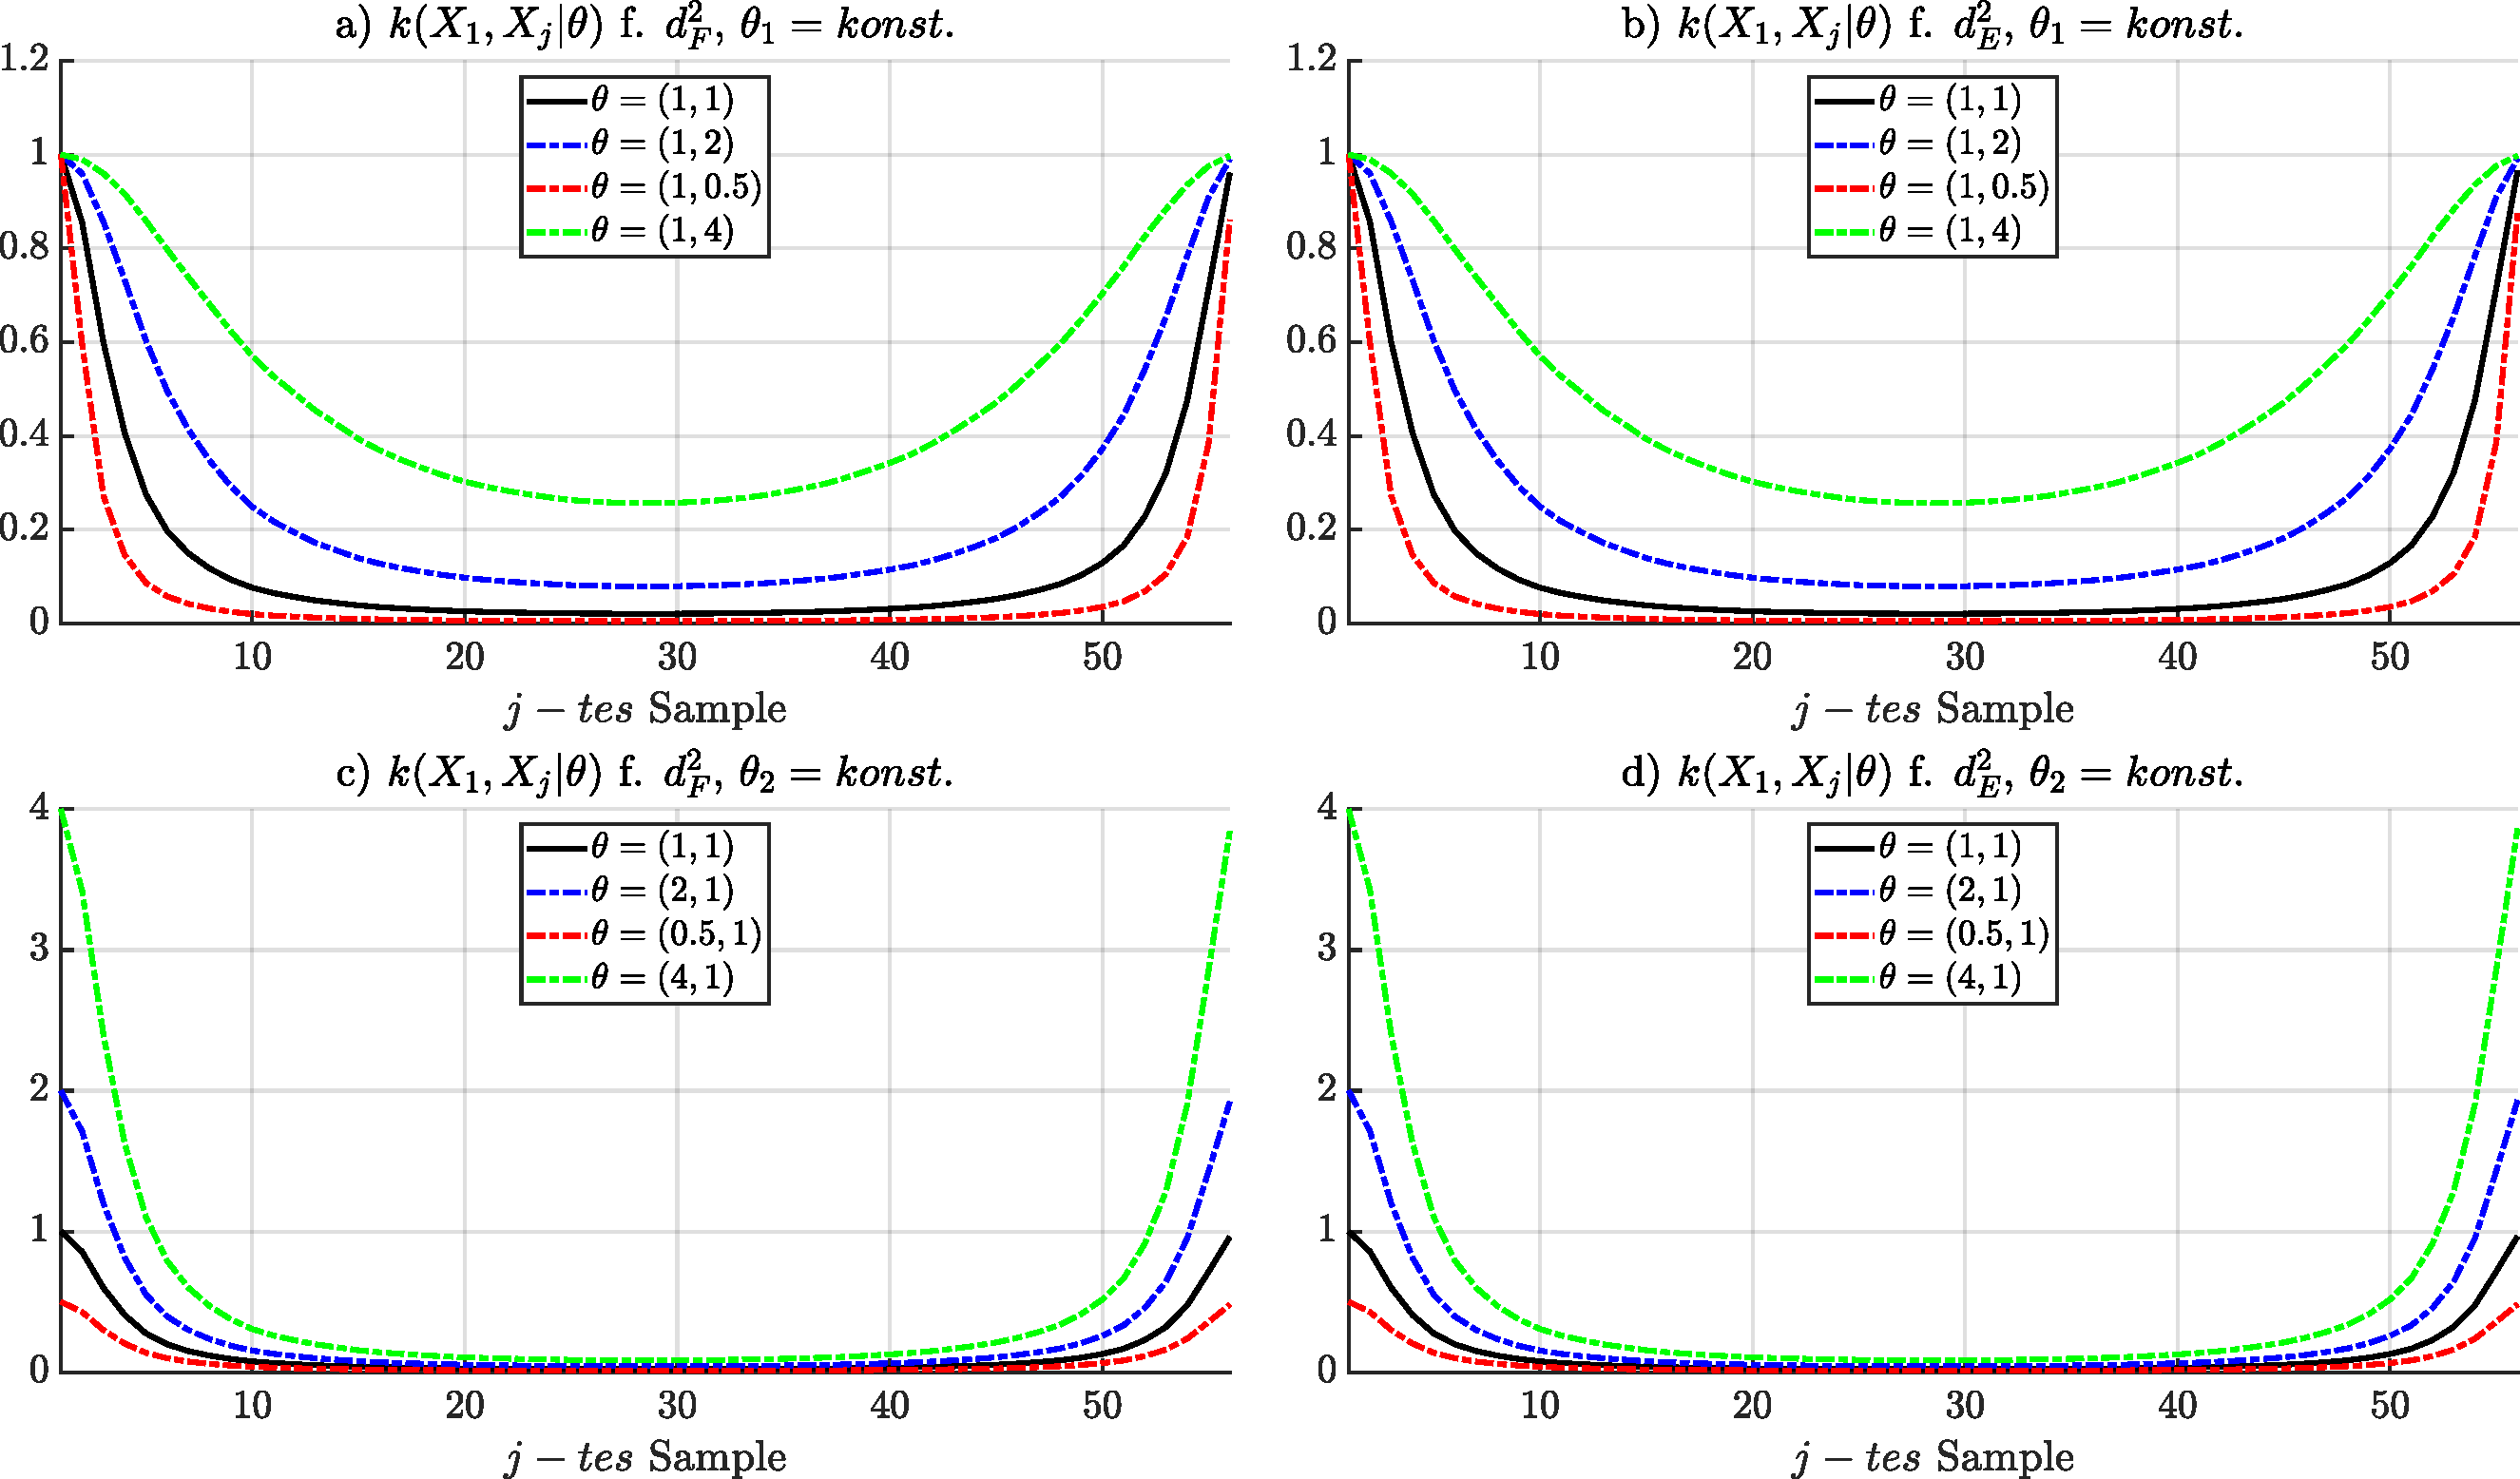
\includegraphics[width=\linewidth]{appendix/images/8-Ergebnisse-Experimente/Vergleich-Kovarianzfunktionen}
	\caption[Kovarianzfunktionen im Vergleich]{Kovarianzfunktionen im Vergleich für variierende Kernel-Parameter $\theta = (\sigma_f^2, \sigma_l)$ und $N=56$ Observerierungen.}
	\label{fig:vergleich-kovarianzfunktionen}
\end{figure}



\begin{figure}[tbph]
	\centering
	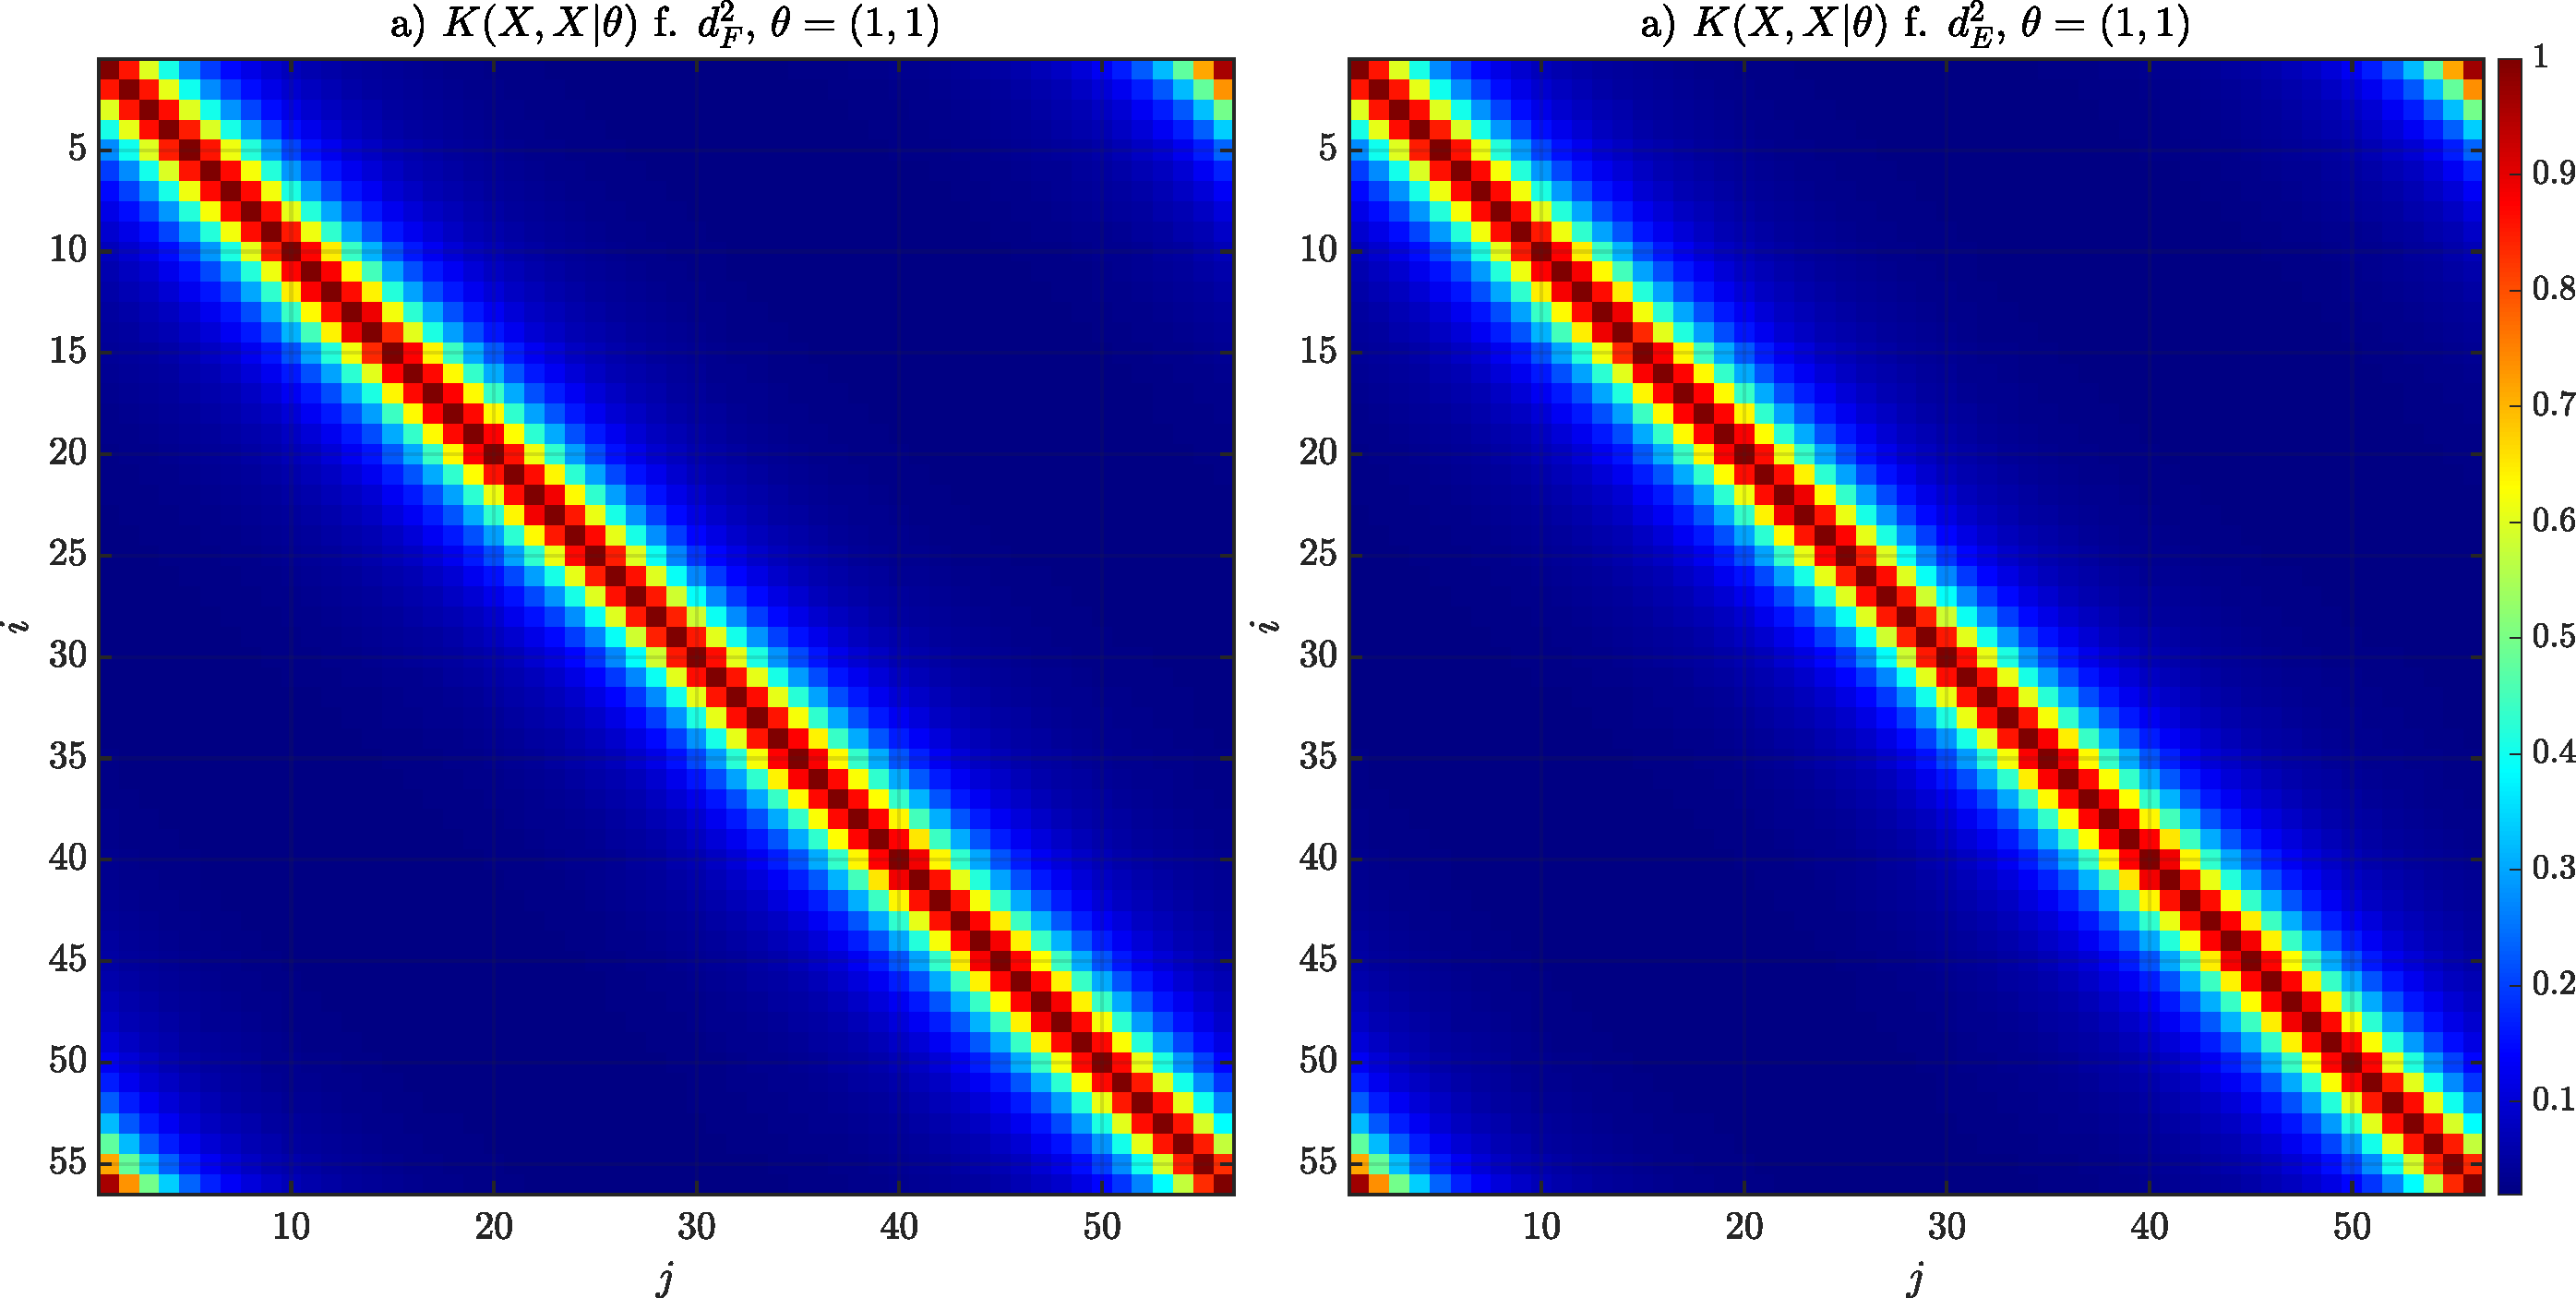
\includegraphics[width=\linewidth]{appendix/images/8-Ergebnisse-Experimente/Vergleich-Kovarianzmatrizen}
	\caption[Gegenüberstellung der Kovarianzmatrizen]{Gegenüberstellung der Kovarianzmatrizen bei ausgeschalter Längen- und und Breitenskalierung mit $\theta = (1,1)$ und $N=56$ Observerierungen.}
	\label{fig:vergleich-kovarianzmatrizen}
\end{figure}


\begin{figure}[tbph]
	\centering
	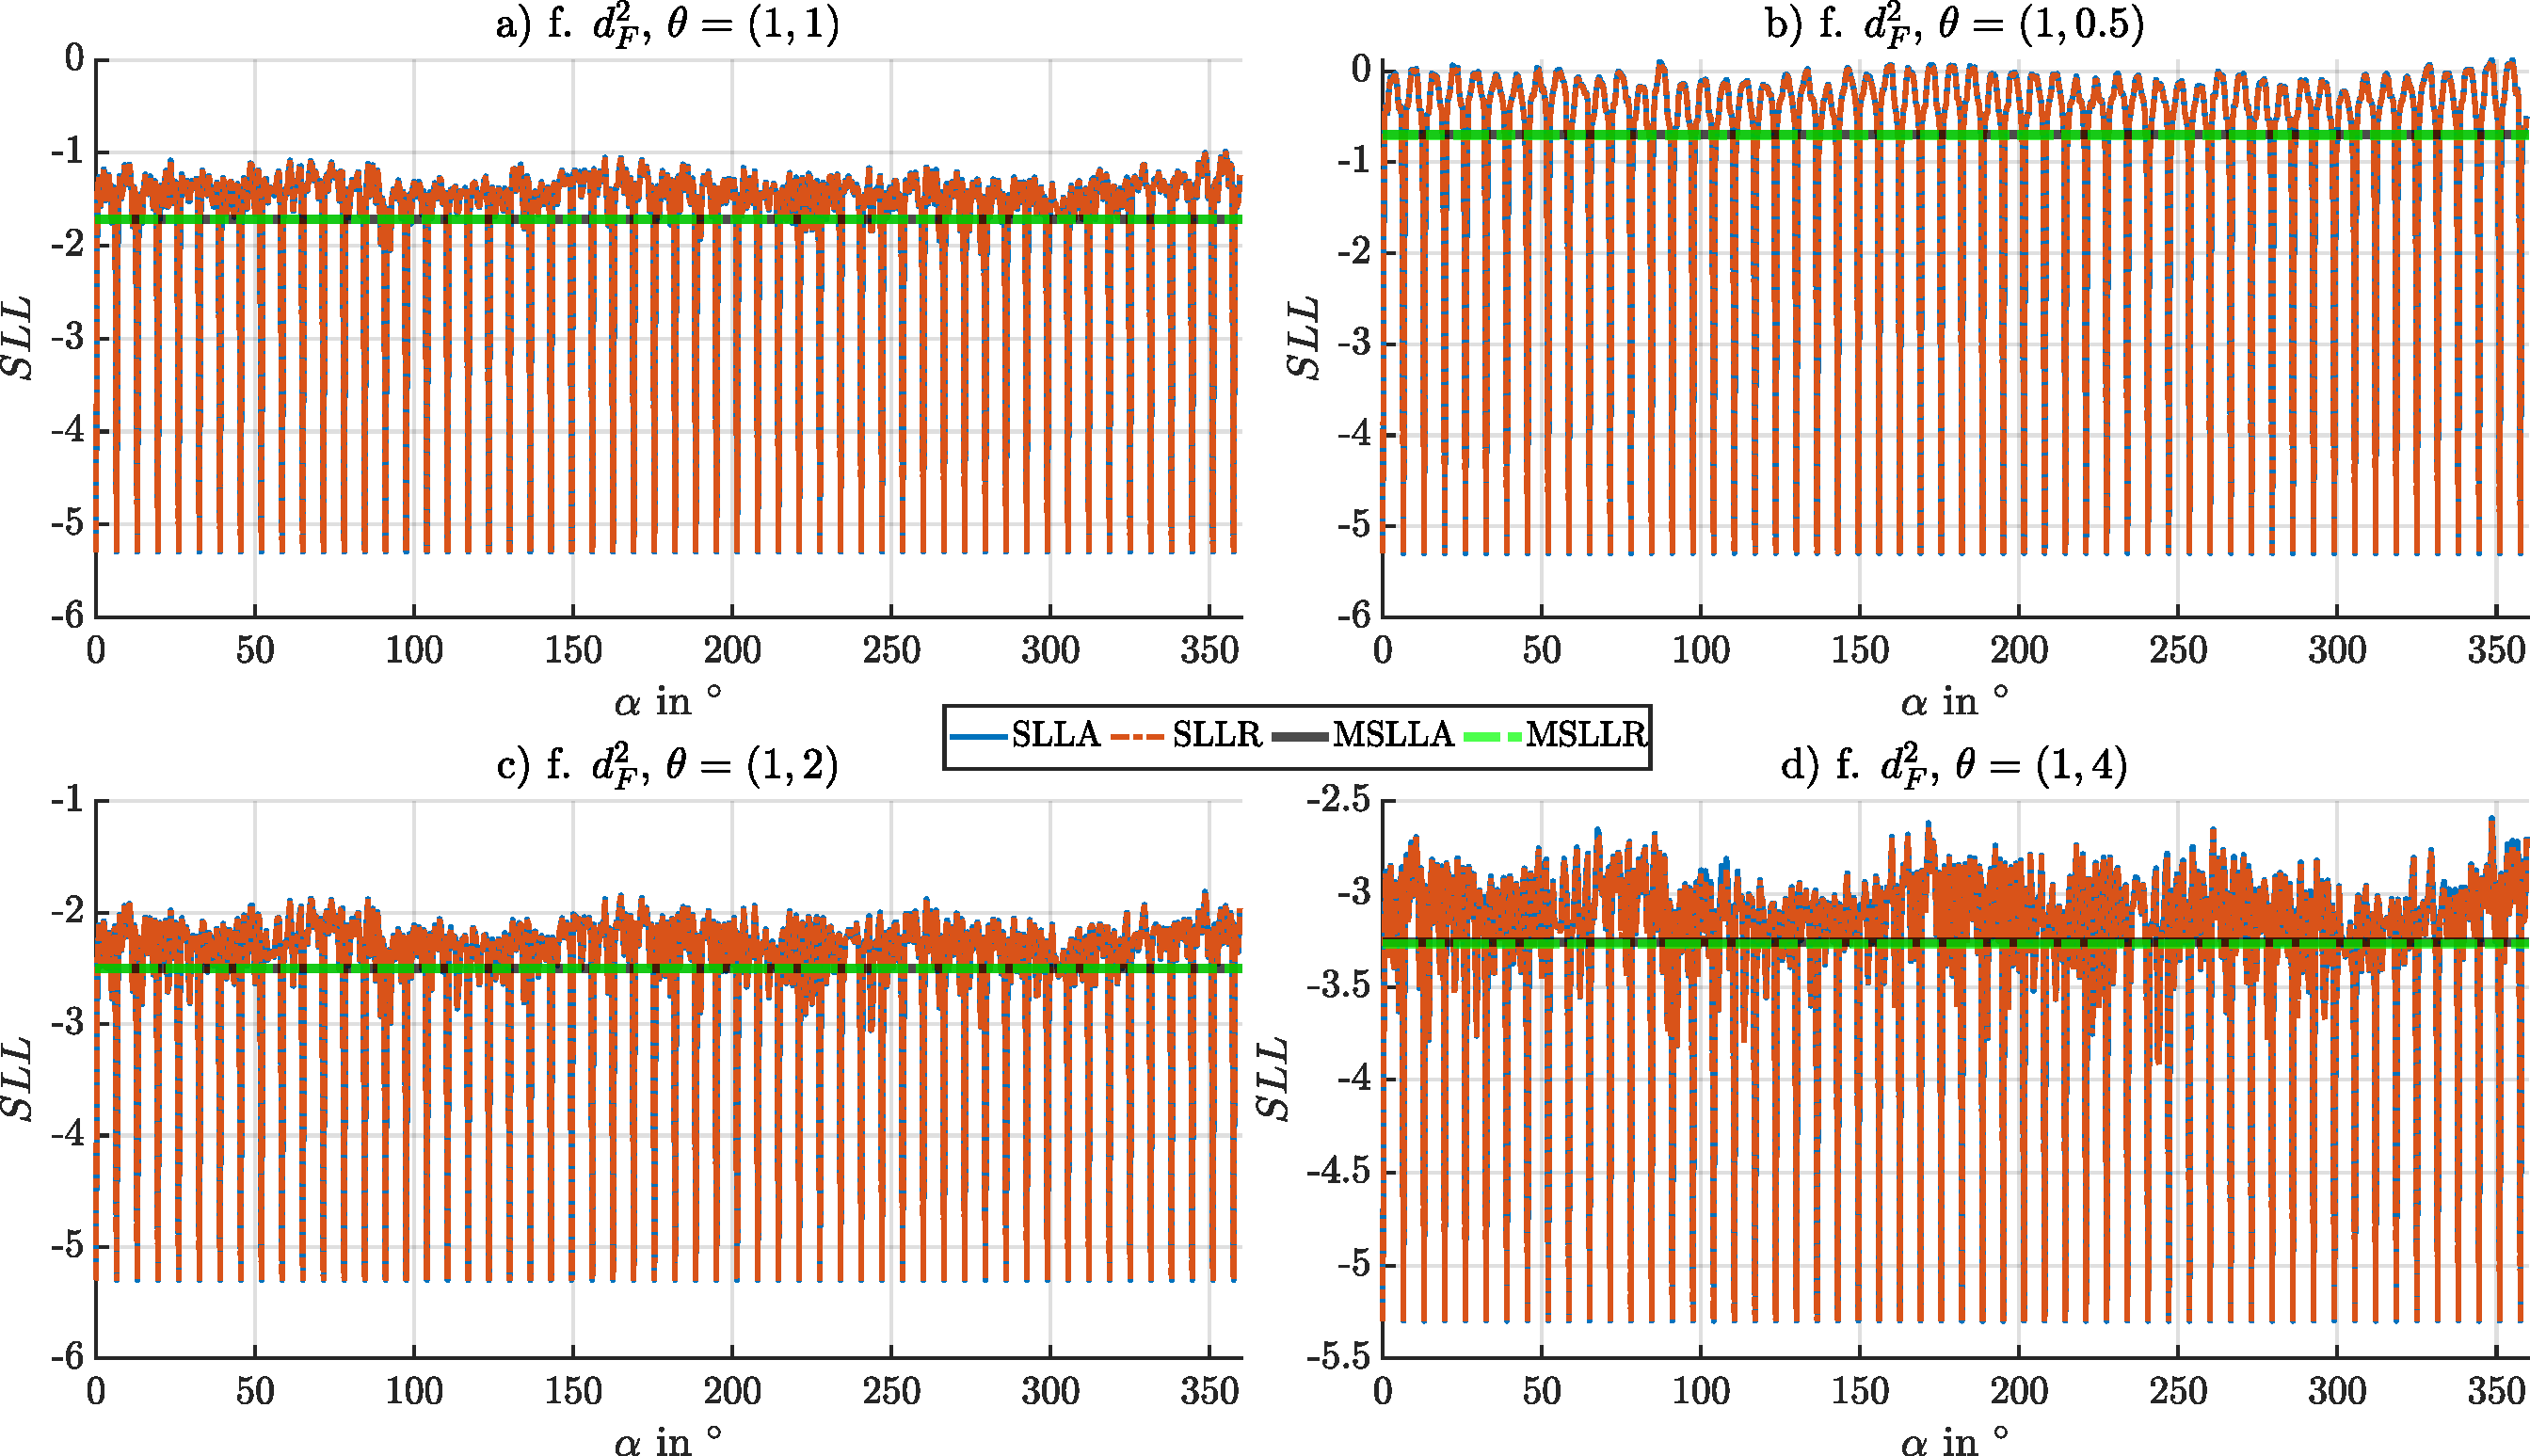
\includegraphics[width=\linewidth]{appendix/images/8-Ergebnisse-Experimente/Vergleich-QFC-SLL}
	\caption[Vergleich der Modellverluste nach Winkel und Radius für die erste Kovarianzfunktion]{Vergleich der Modellverluste nach Winkel und Radius für die erste Kovarianzfunktion für variierende Breitenskalierung.}
	\label{fig:vergleich-qfc-sll}
\end{figure}


\begin{figure}[tbph]
	\centering
	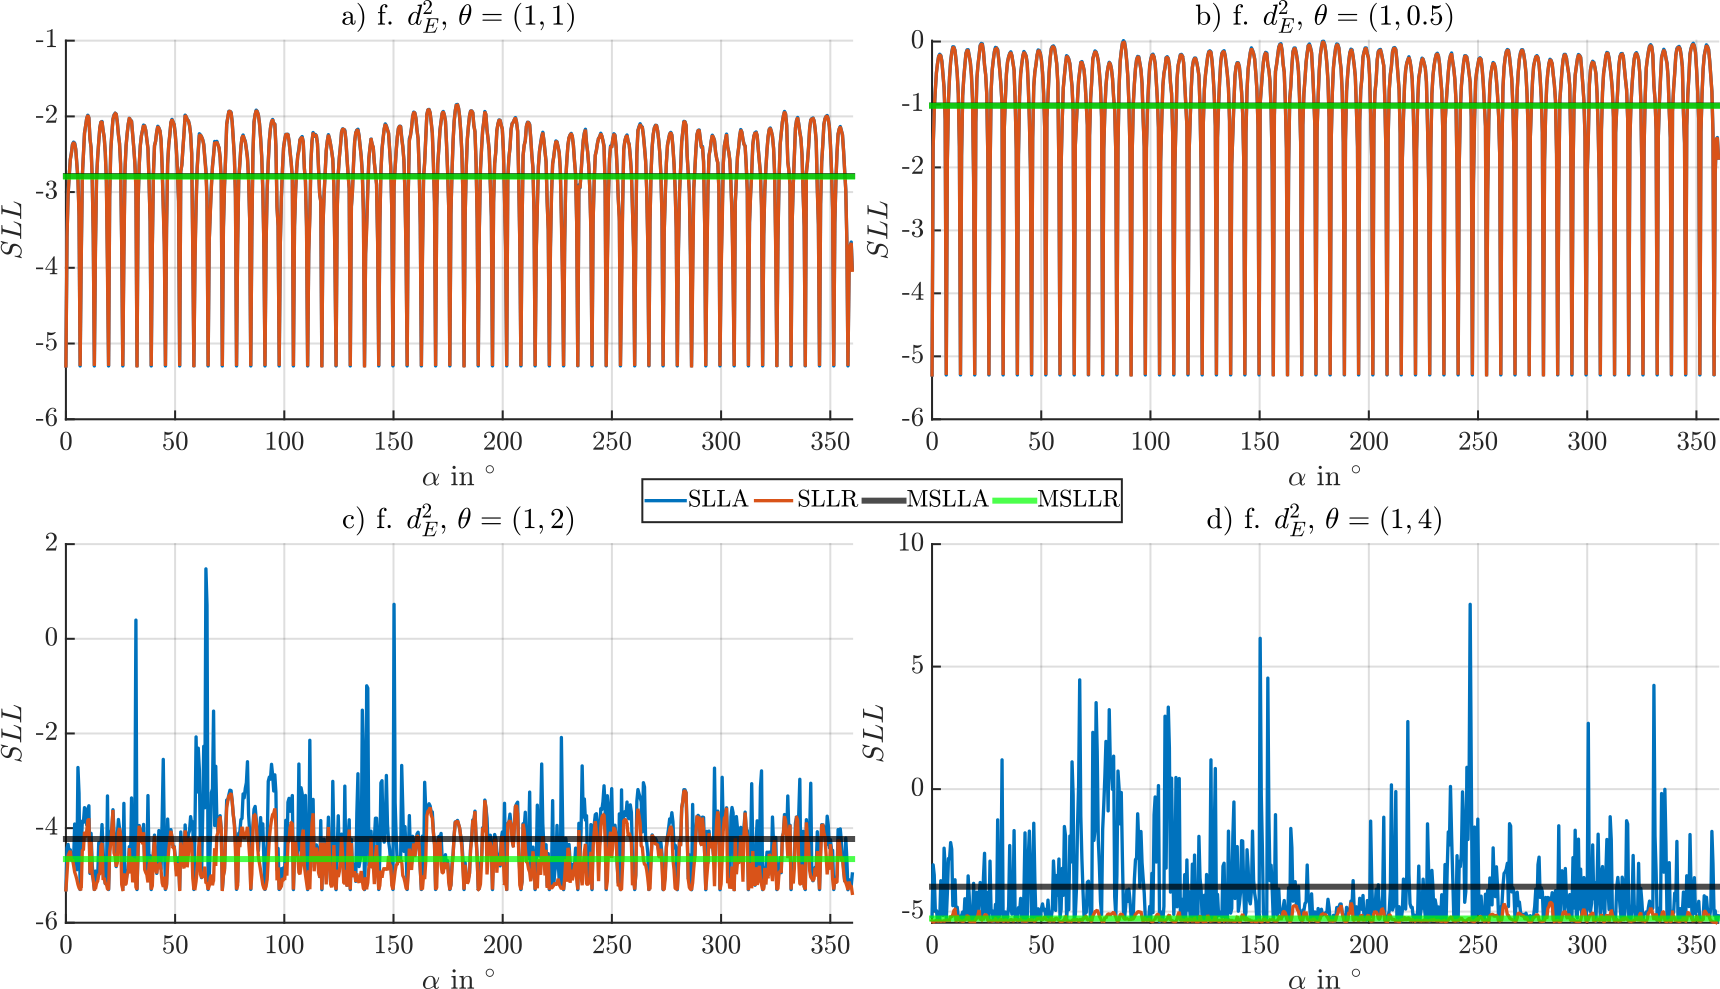
\includegraphics[width=\linewidth]{appendix/images/8-Ergebnisse-Experimente/Vergleich-QFCAPX-SLL}
	\caption[Vergleich der Modellverluste nach Winkel und Radius für die zweite Kovarianzfunktion]{Vergleich der Modellverluste nach Winkel und Radius für die zweite Kovarianzfunktion für variierende Breitenskalierung.}
	\label{fig:vergleich-qfcapx-sll}
\end{figure}


\clearpage


\section{Anpassung der Referenzwinkelanzahl}\label{sec:ergexp2}


\begin{figure}[tbph]
	\centering
	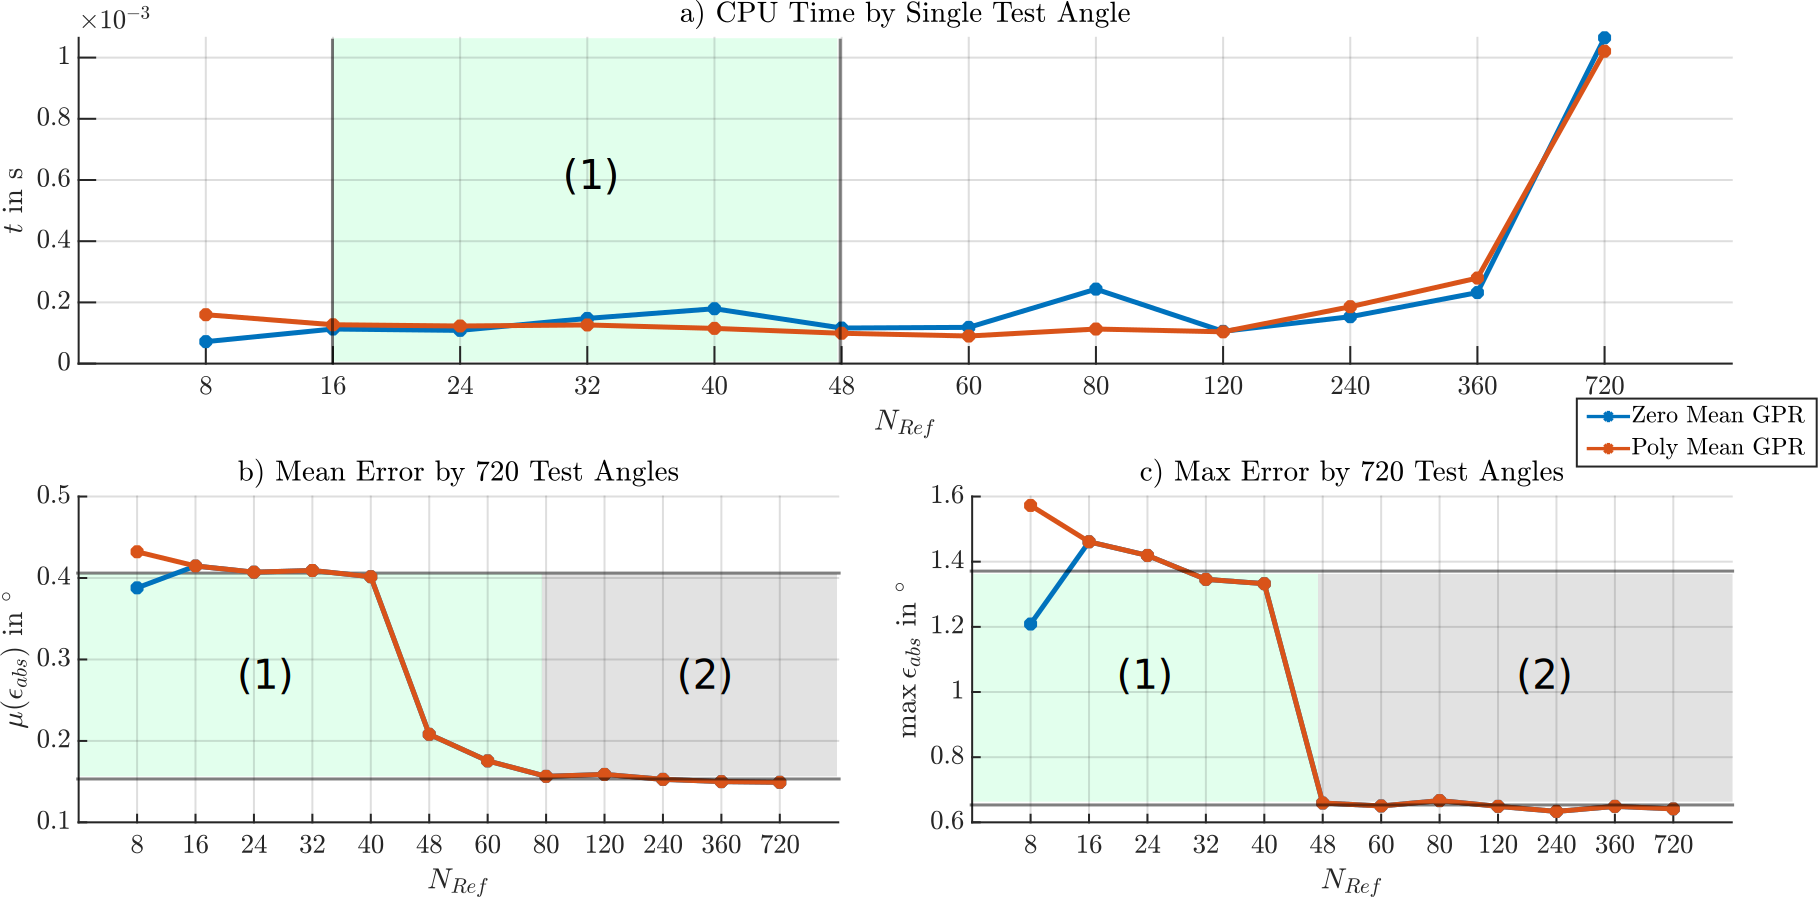
\includegraphics[width=\linewidth]{appendix/images/8-Ergebnisse-Experimente/Timings-vs-Errors}
	\caption[Timing vs Error]{QFCAPX Zero vs Poly 1 Nref Opt 32 (APX) = 8 (QFC) Timing vs Error, Noise Level Gap äußere Optimierung gleicht aus. (1) zu wählender Bereich mit 32 Samples, erfordert Rauschanpassung. (2) Rauschanpassung nicht zwingend notwendig, aber ressourcenintensiv.}
	\label{fig:timings-vs-errors}
\end{figure}


\clearpage


\section{Anpassung des Rauschniveaus}\label{sec:ergexp3}


\begin{figure}[tbph]
	\centering
	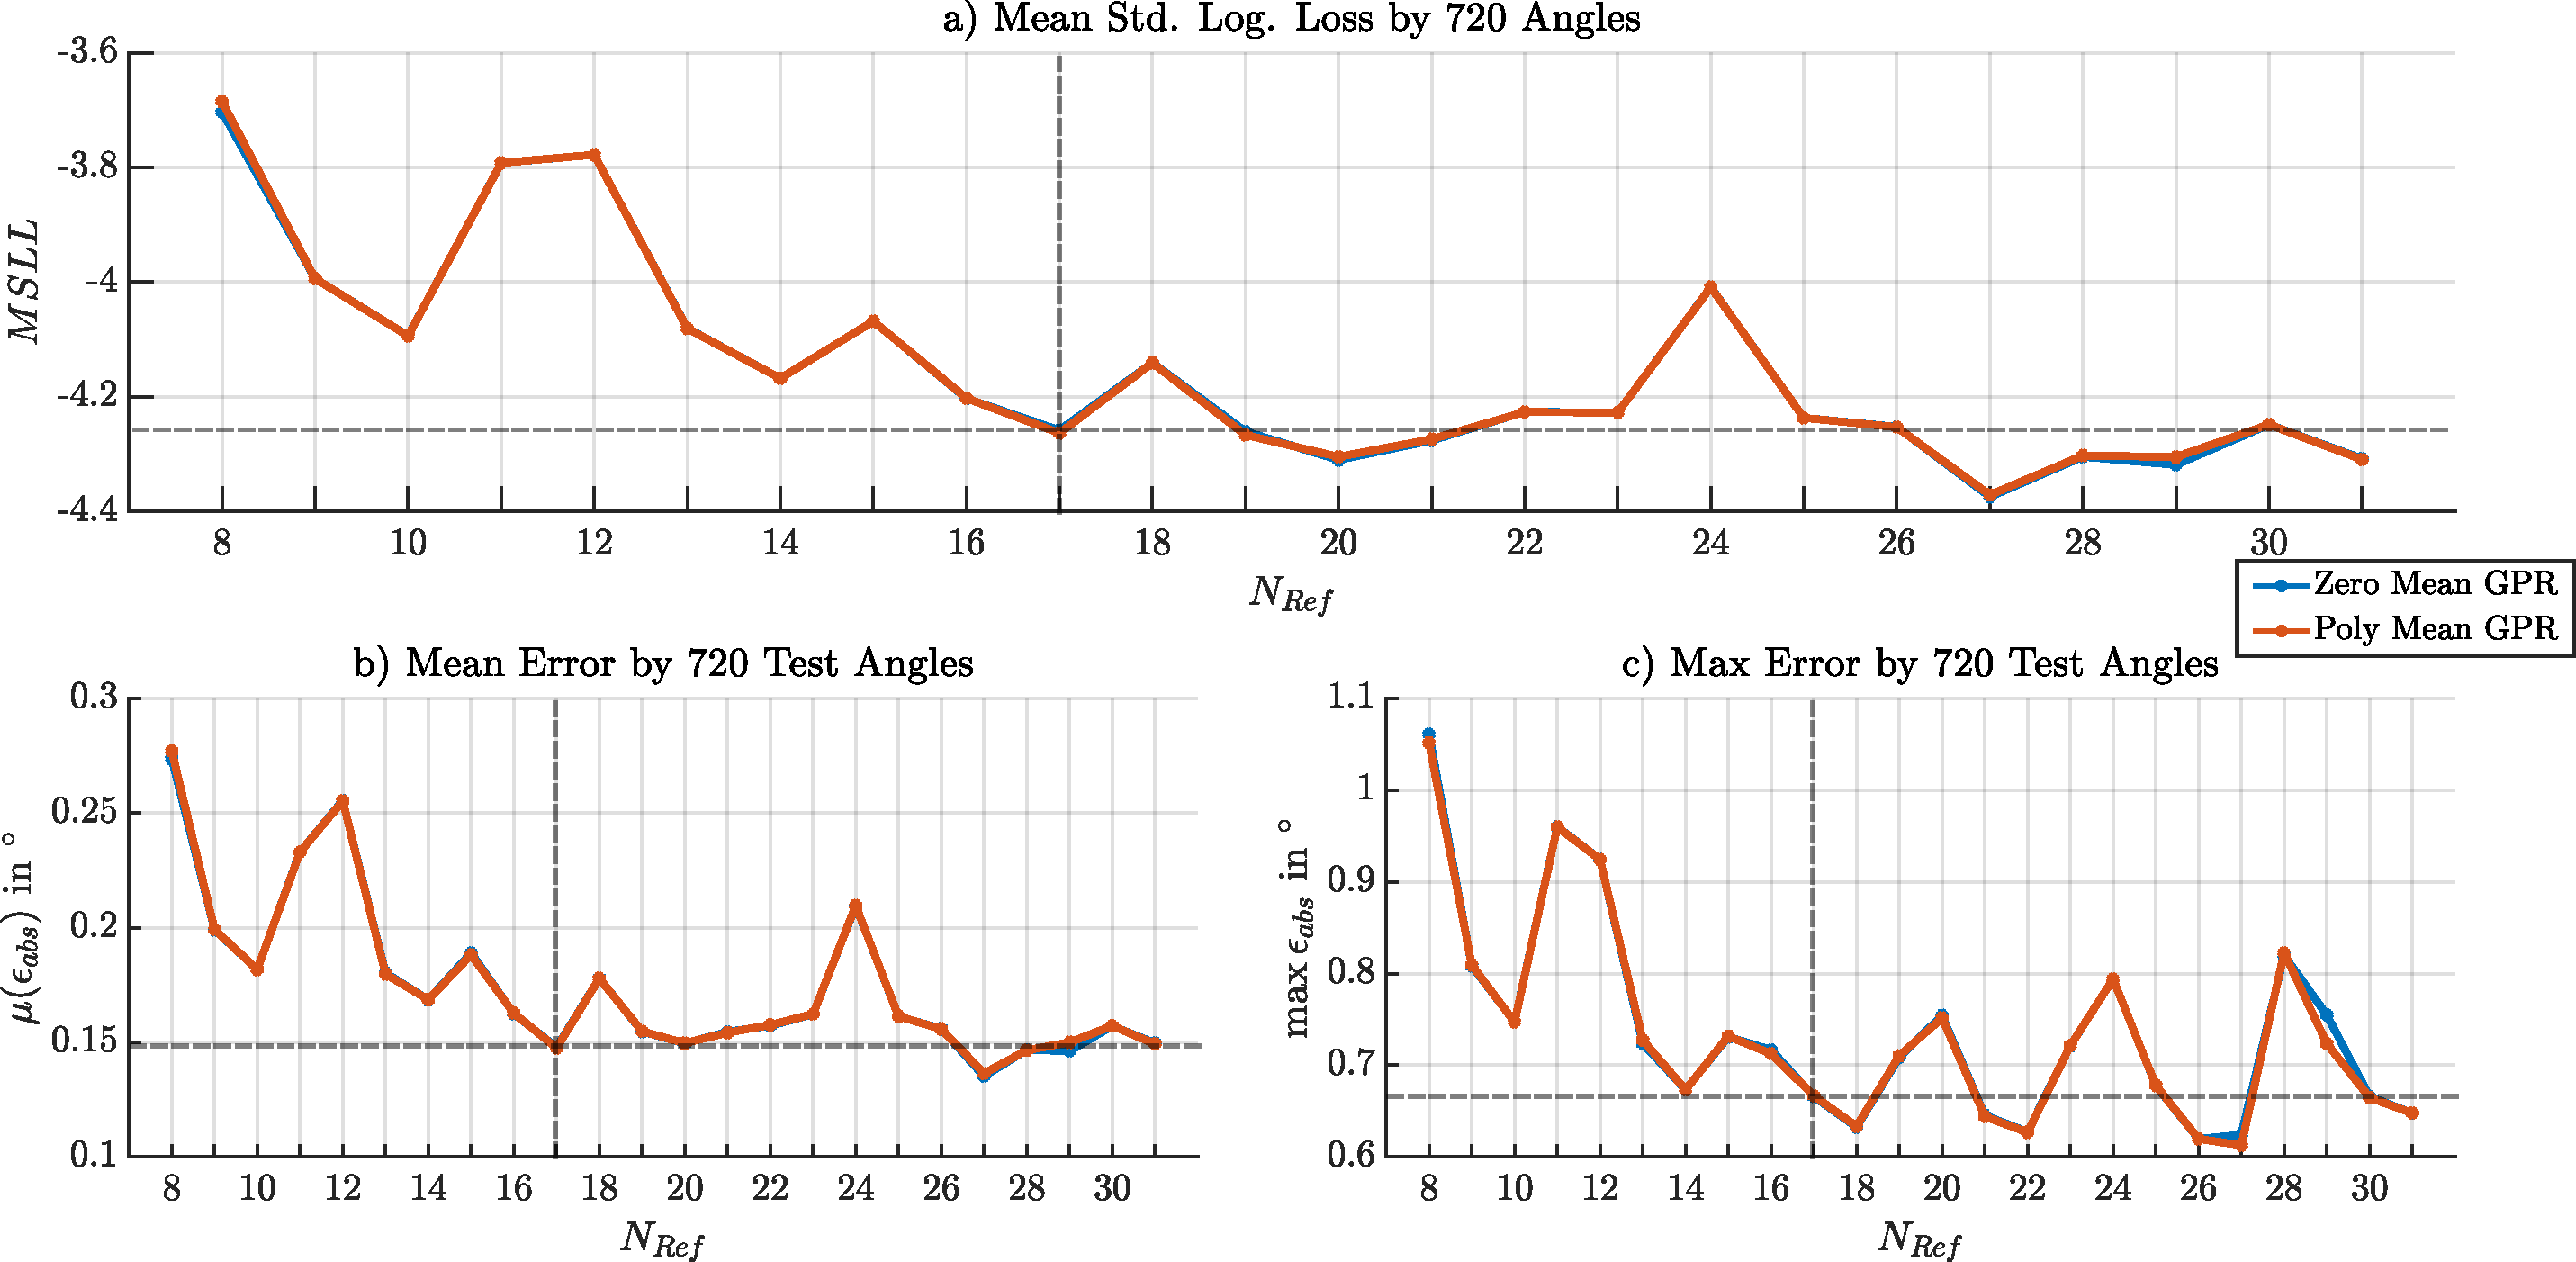
\includegraphics[width=\linewidth]{appendix/images/8-Ergebnisse-Experimente/MSLL-vs-Errors}
	\caption[MSLL vs Error für Nref 17]{MSLL vs Error für Nref 17 Kompromiss}
	\label{fig:msll-vs-errors}
\end{figure}


\clearpage


\section{Anpassung der Parametergrenzen}\label{sec:ergexp4}

Anpassung:

$\sigma_f^2$-Bounds: $(1, 10)$ / $\sigma_l$-Bounds: $(10, 30)$ / $\sigma_n^2$-Bounds: $(10^{-6}, 10^{-4})$


\begin{figure}[tbph]
	\centering
	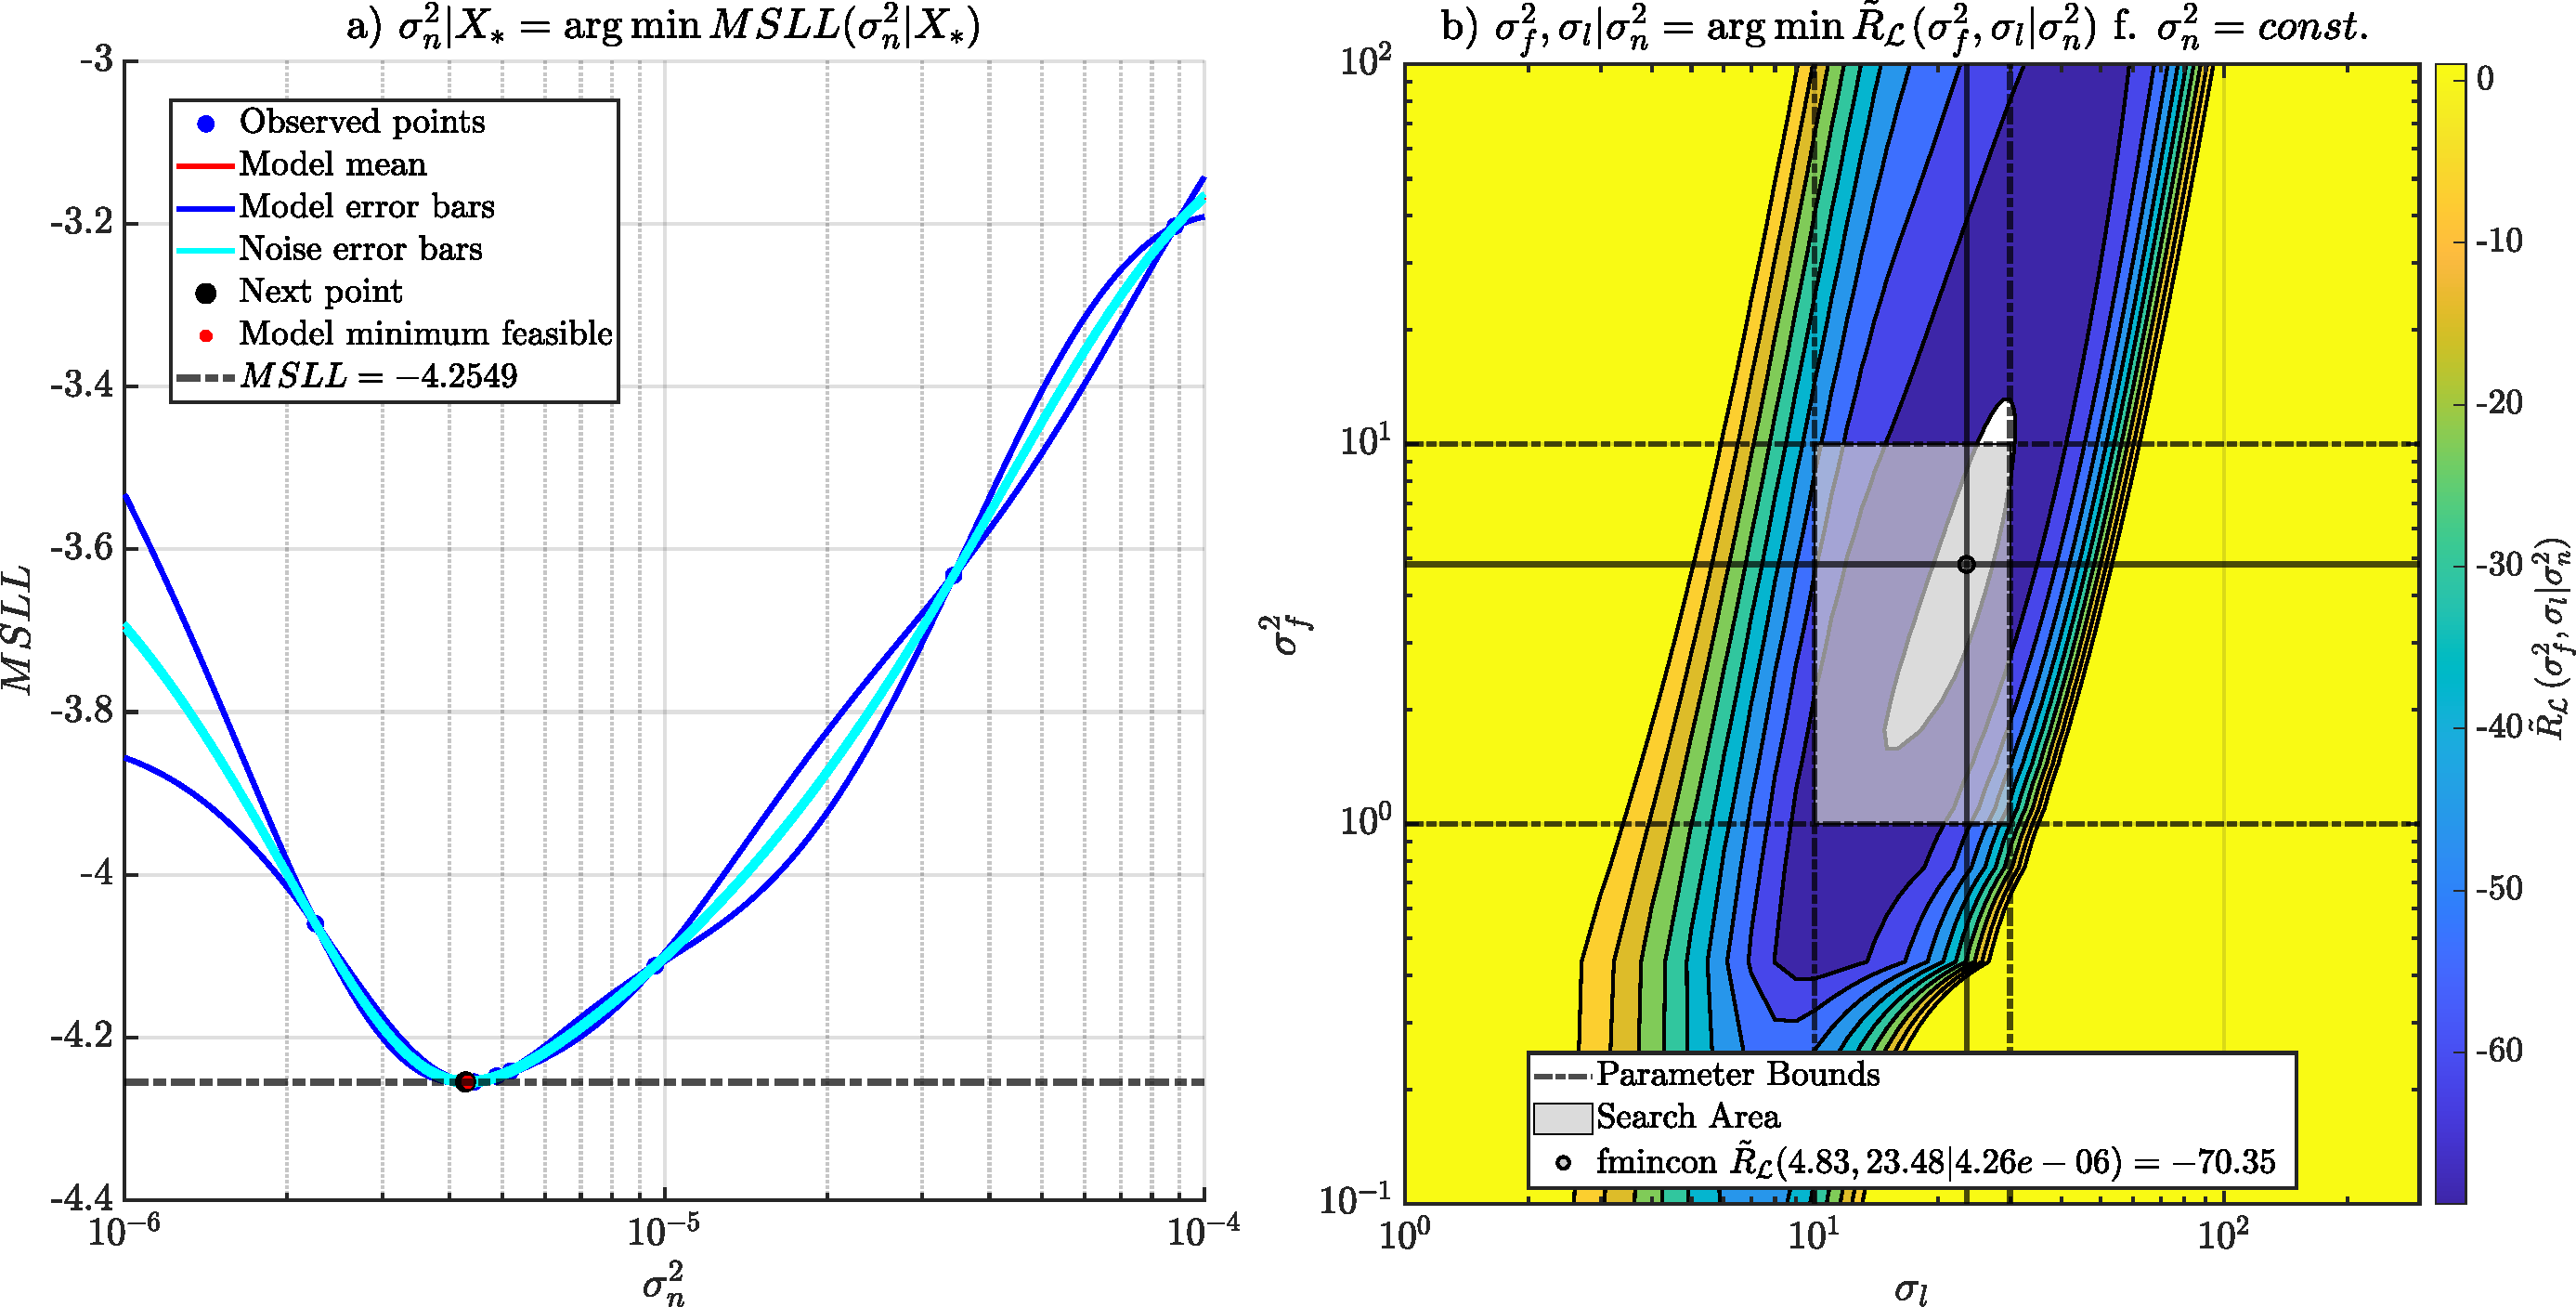
\includegraphics[width=\linewidth]{appendix/images/8-Ergebnisse-Experimente/QFCAPX-Z-N17-Bounds}
	\caption[Angepaster Parameter Bounds]{Angepaster Parameter Bounds}
	\label{fig:qfcapx-z-n17-bounds}
\end{figure}


Anpassung: Durchlaufzahl 10


\begin{figure}[tbph]
	\centering
	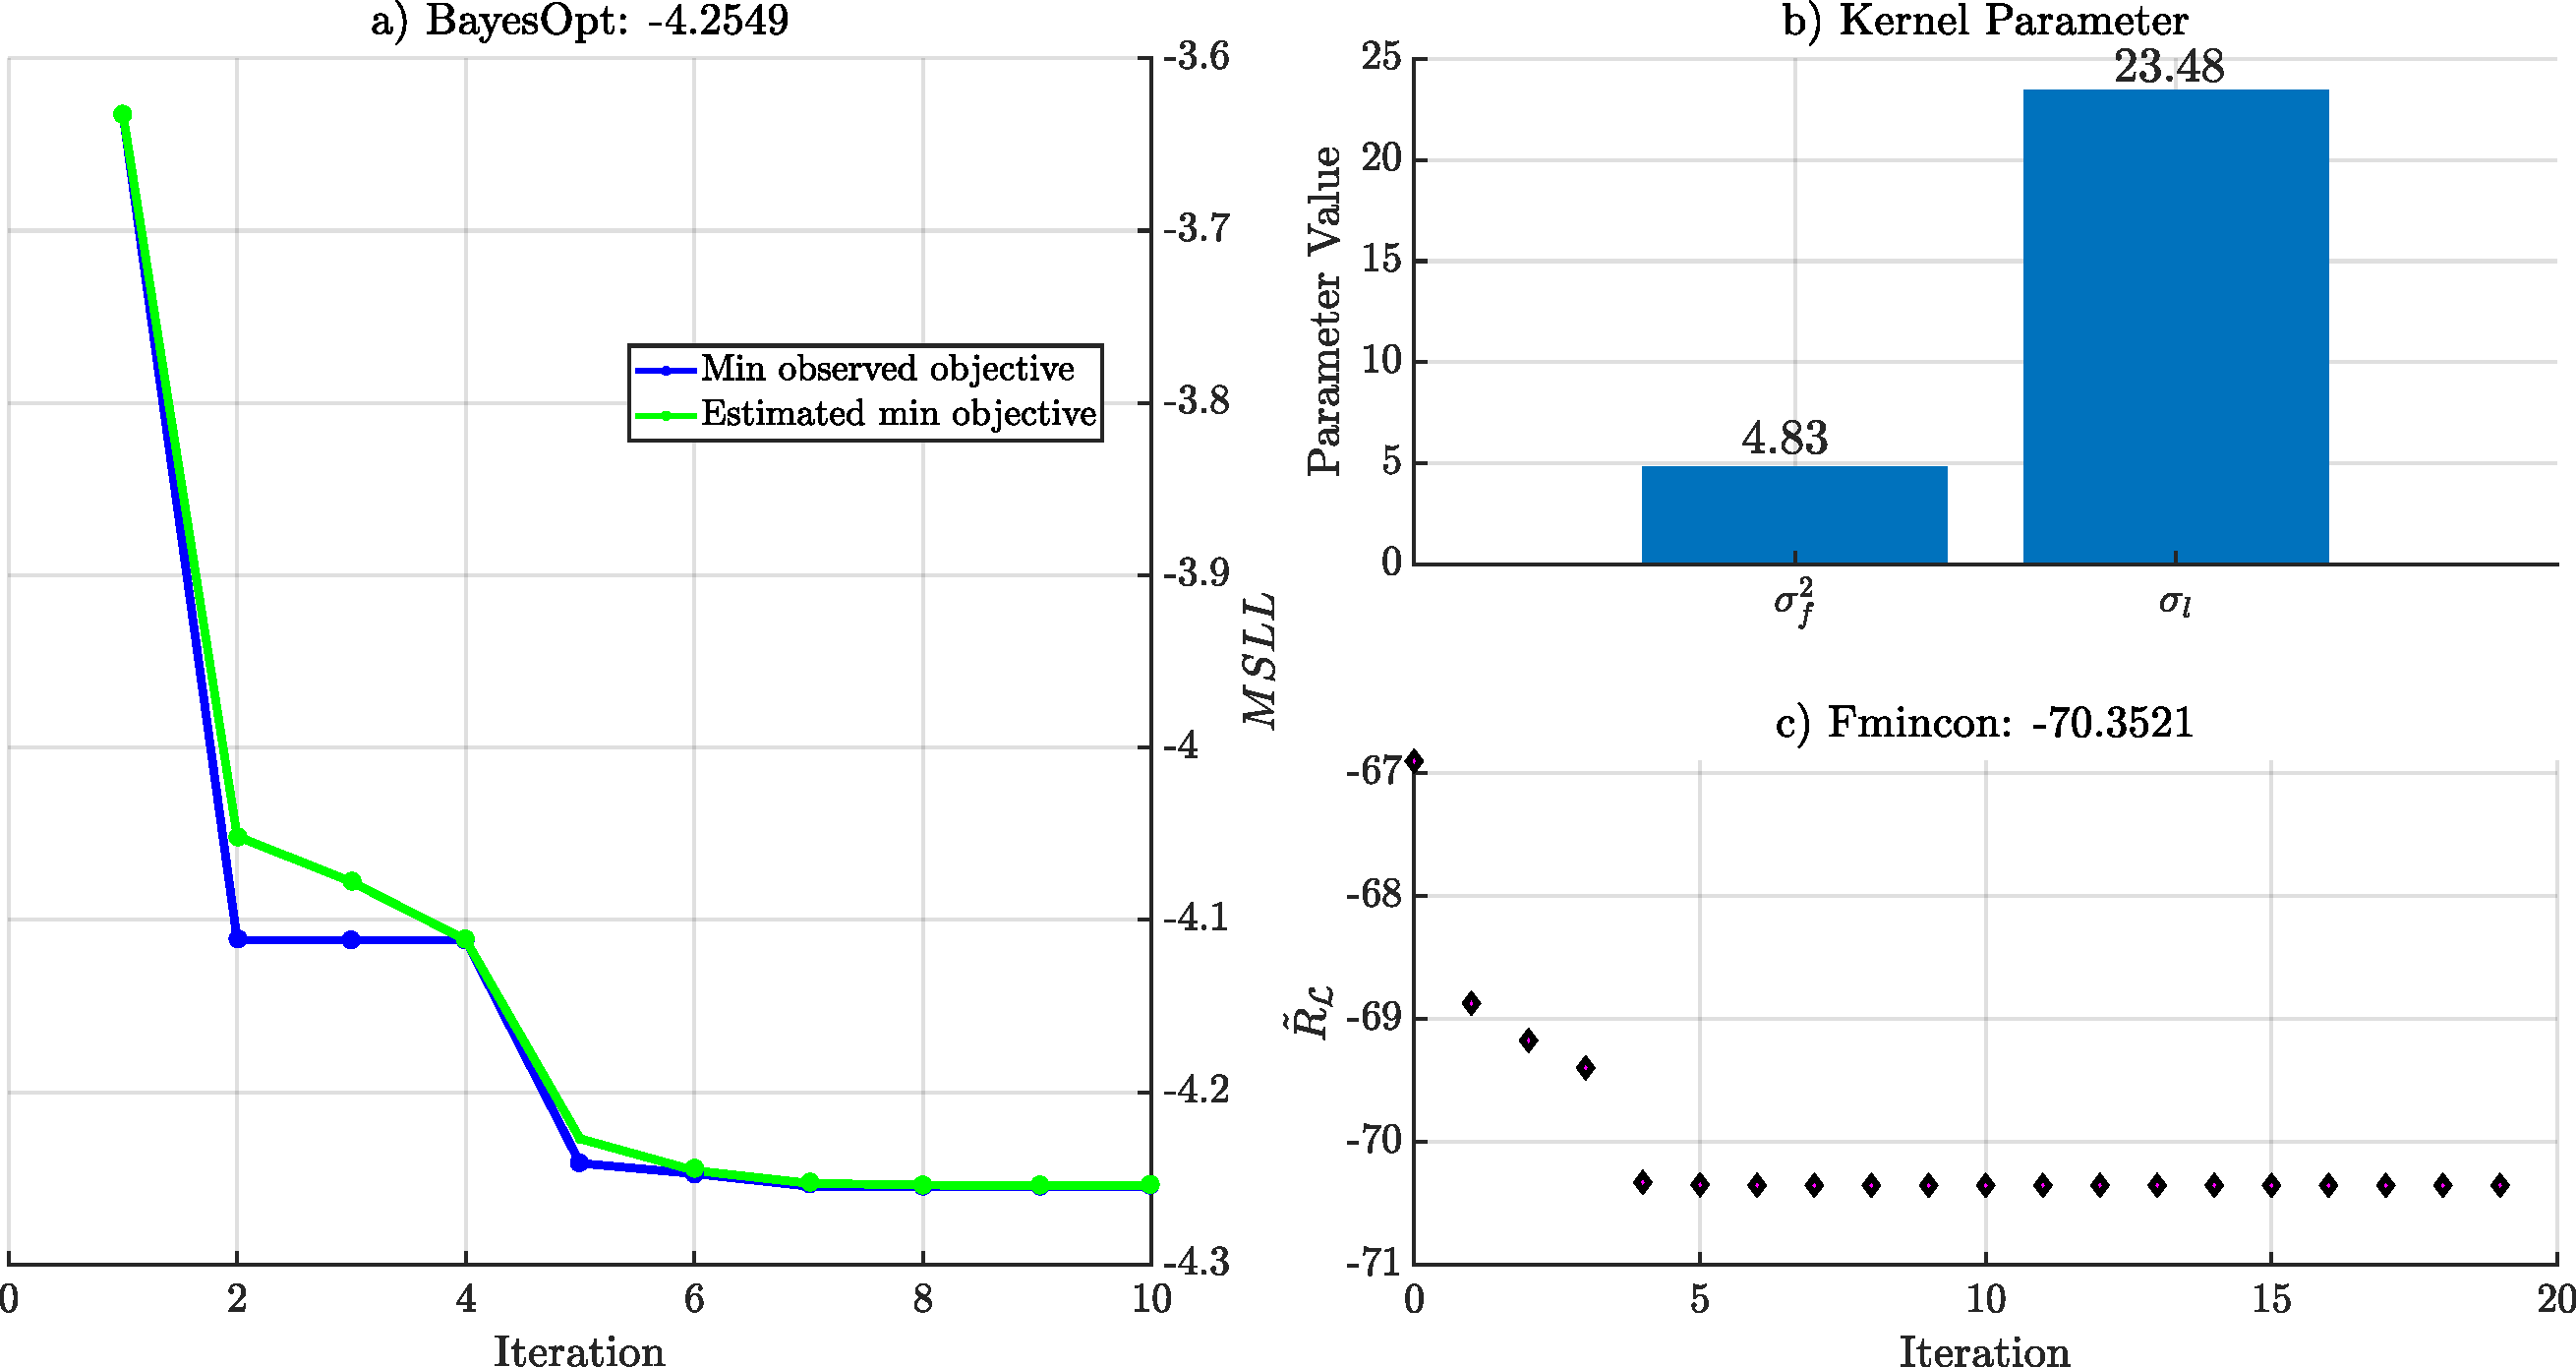
\includegraphics[width=\linewidth]{appendix/images/8-Ergebnisse-Experimente/QFCAPX-Z-N17-Opt}
	\caption[QFCAPX Z N17 Optimierung Runs 10]{QFCAPX Z N17 Optimierung Runs 10}
	\label{fig:qfcapx-z-n17-opt}
\end{figure}





\clearpage


\section{Verhalten bei einfachen Fehllagen}\label{sec:ergexp5}


\begin{figure}[tbph]
	\centering
	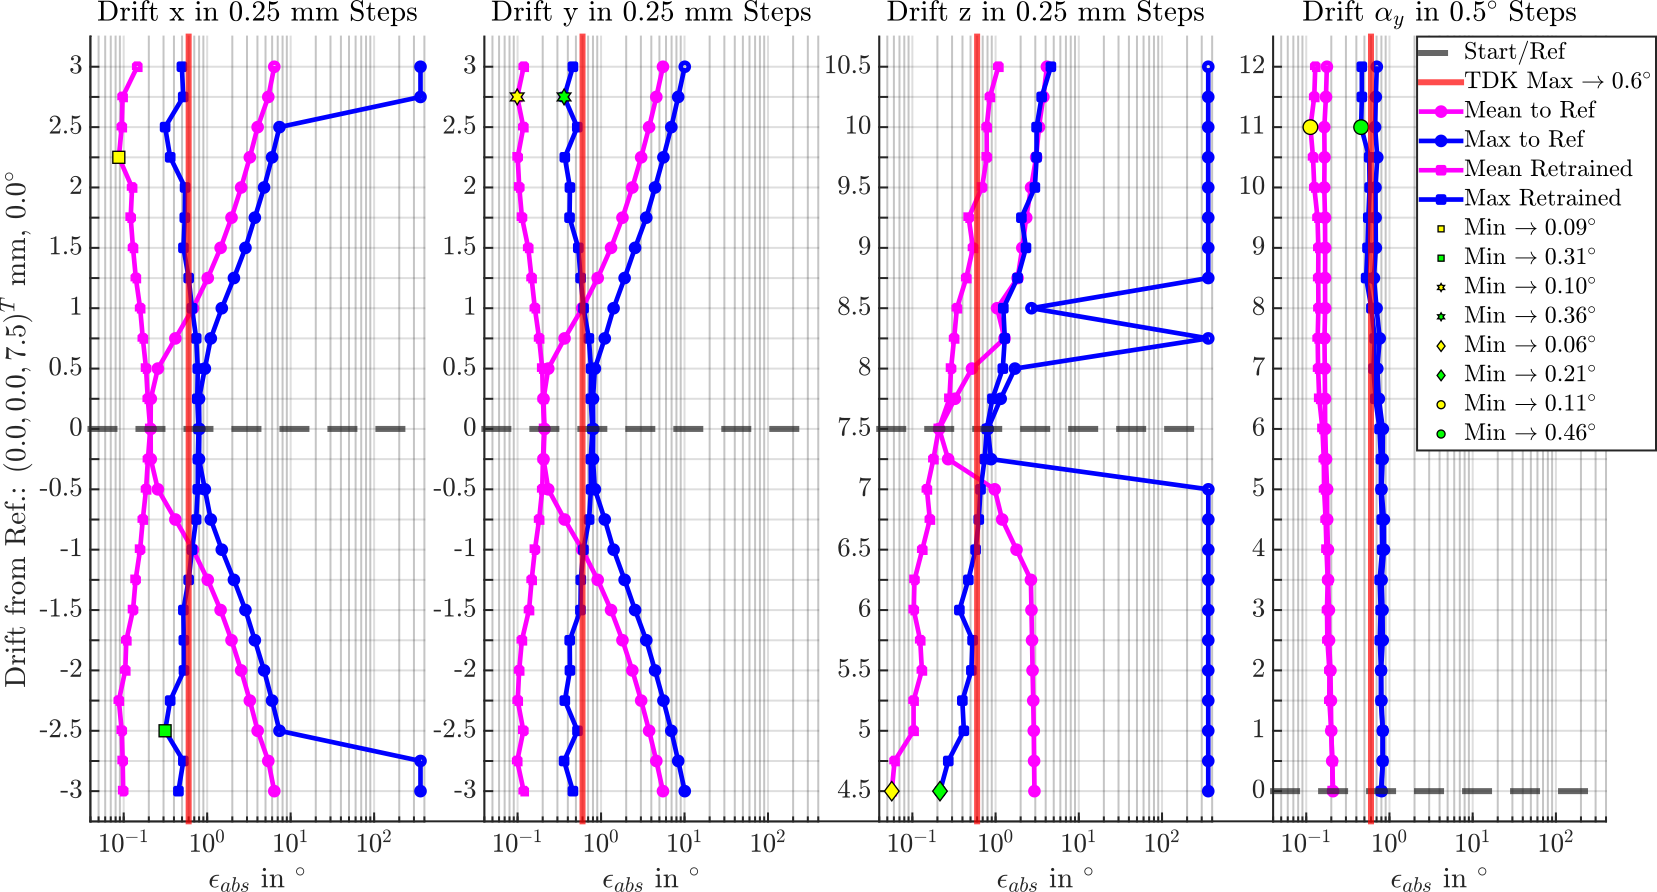
\includegraphics[width=\linewidth]{appendix/images/8-Ergebnisse-Experimente/Drift-Model-Errors}
	\caption[Drift xyz tilt mean max errors 2 ref and retrained]{Drift xyz tilt mean max errors 2 ref and retrained}
	\label{fig:drift-model-errors}
\end{figure}


\begin{figure}[tbph]
	\centering
	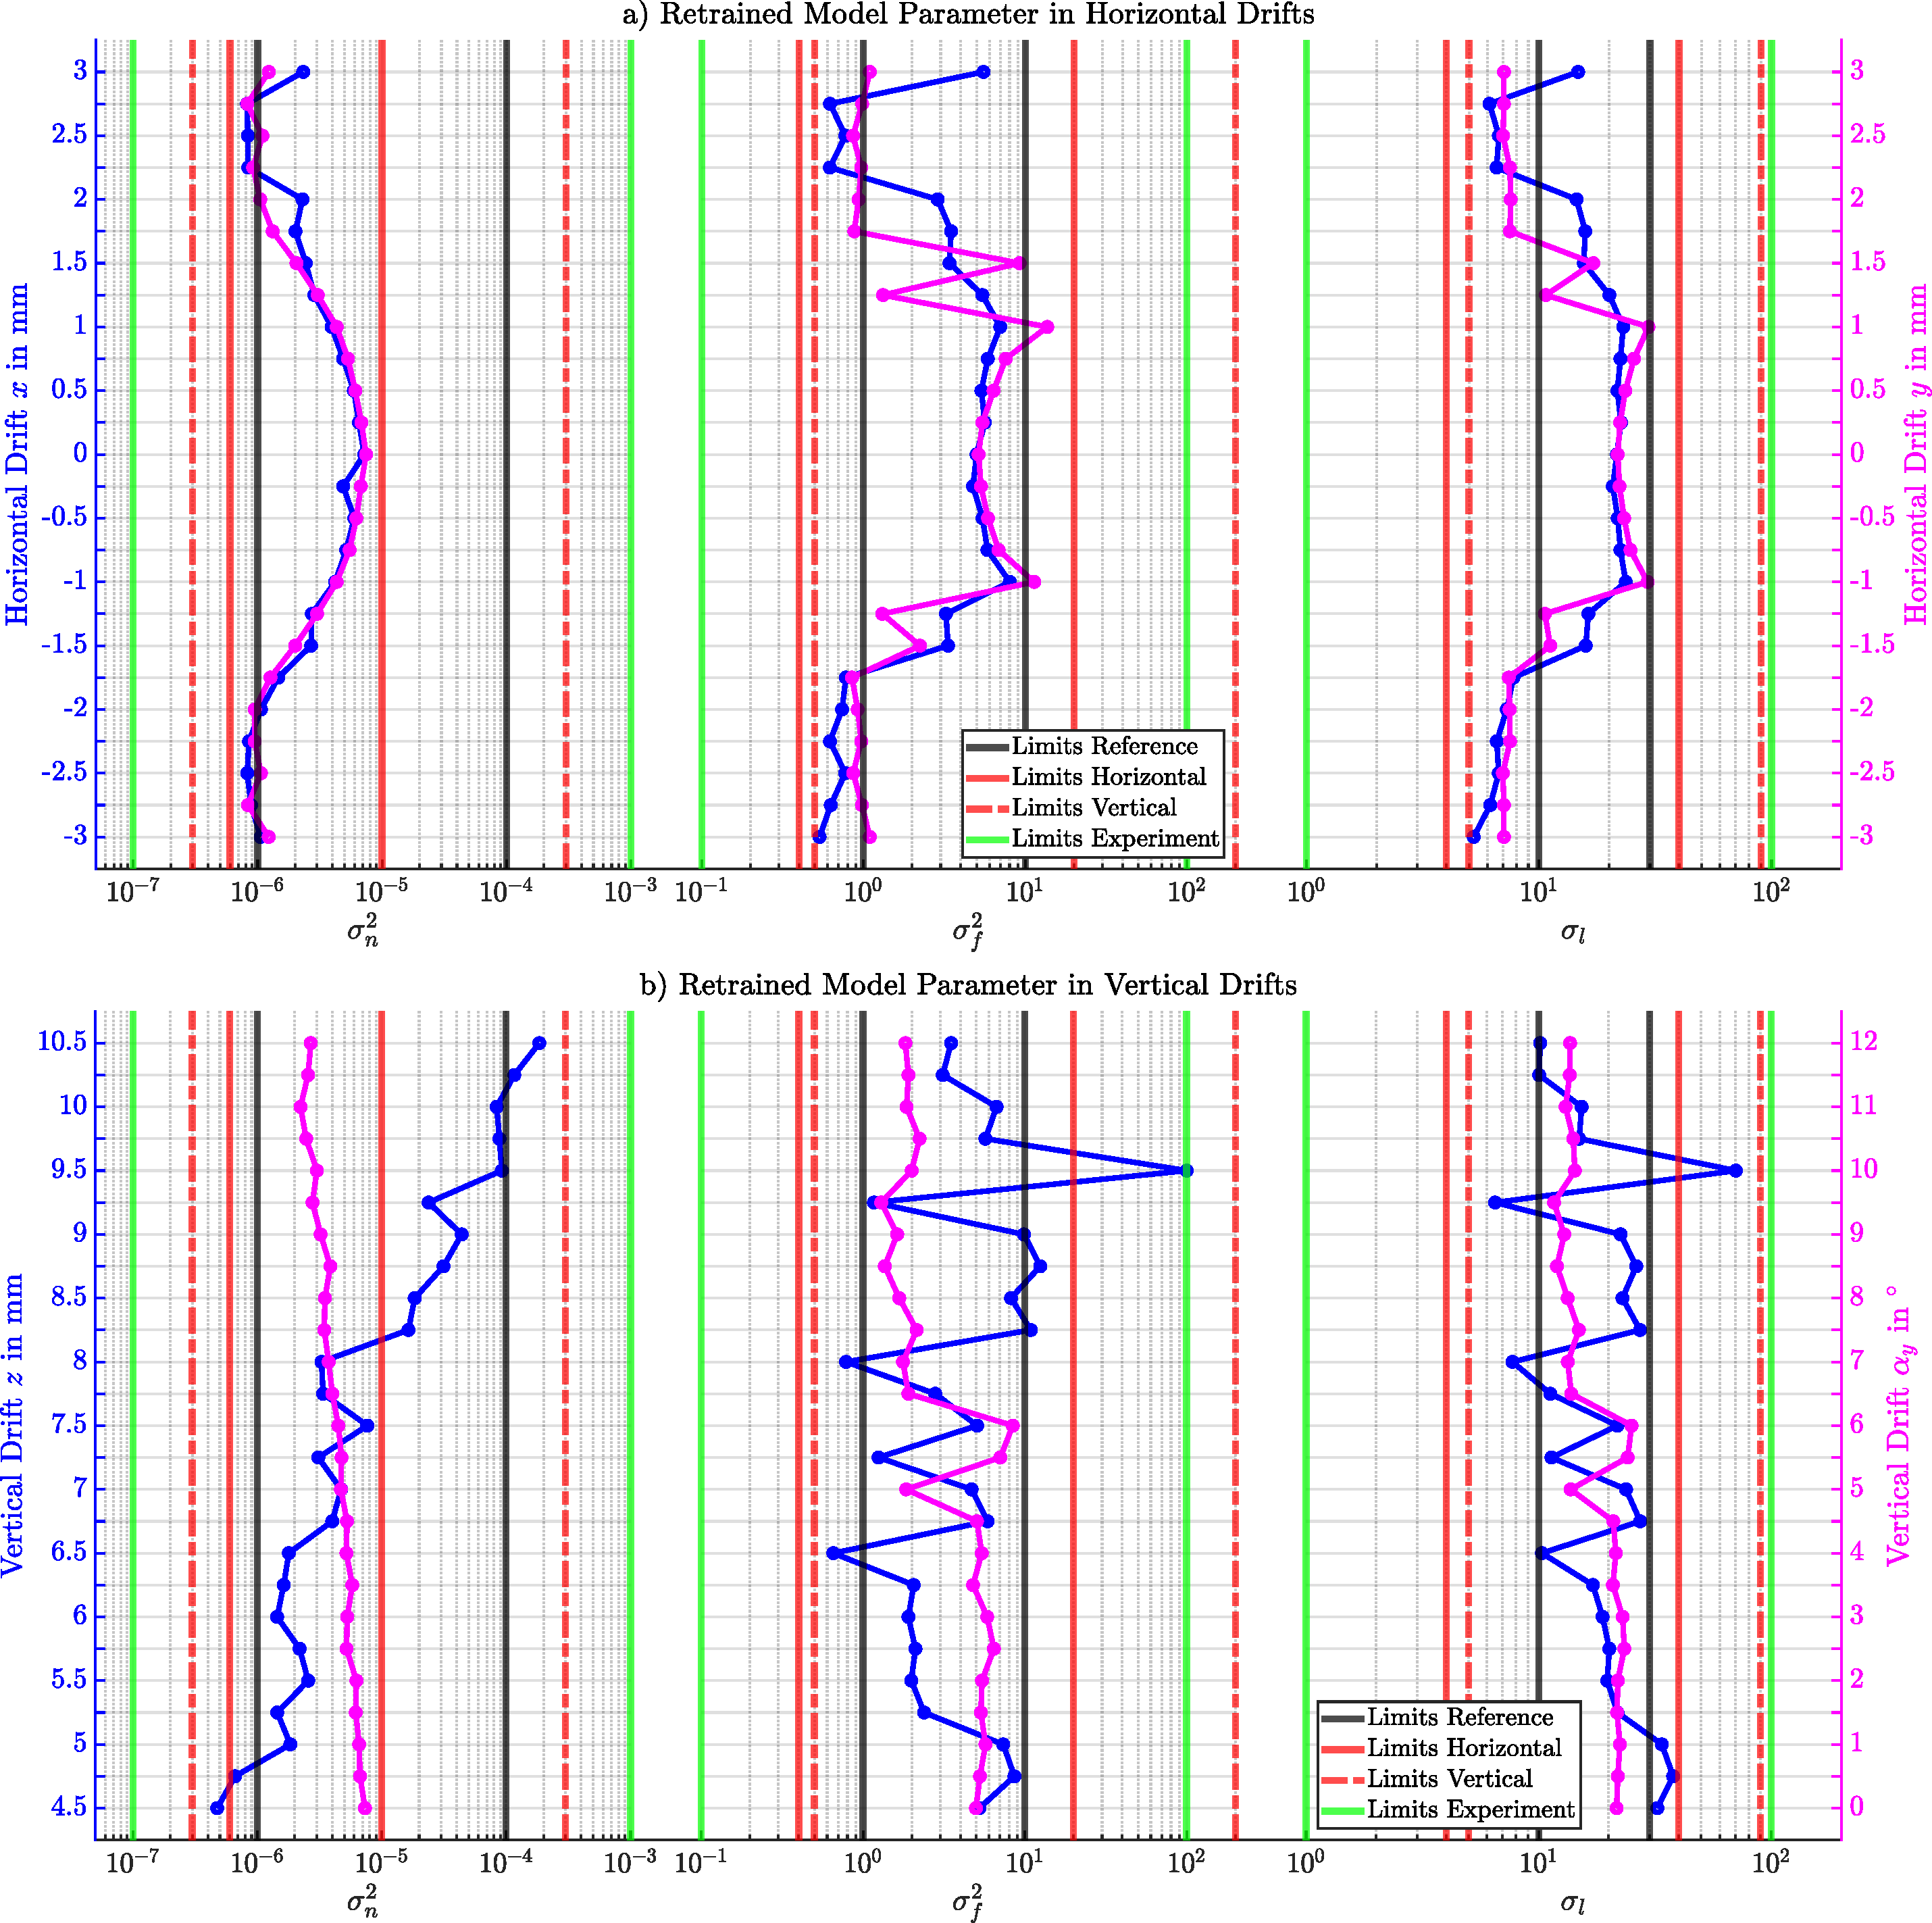
\includegraphics[width=\linewidth]{appendix/images/8-Ergebnisse-Experimente/Drift-Model-Parms}
	\caption[Drift xyz tilt retrained model params tracking]{Drift xyz tilt retrained model params tracking, limits from exp and ref and new suggestion}
	\label{fig:drift-model-parms}
\end{figure}


\begin{figure}[tbph]
	\centering
	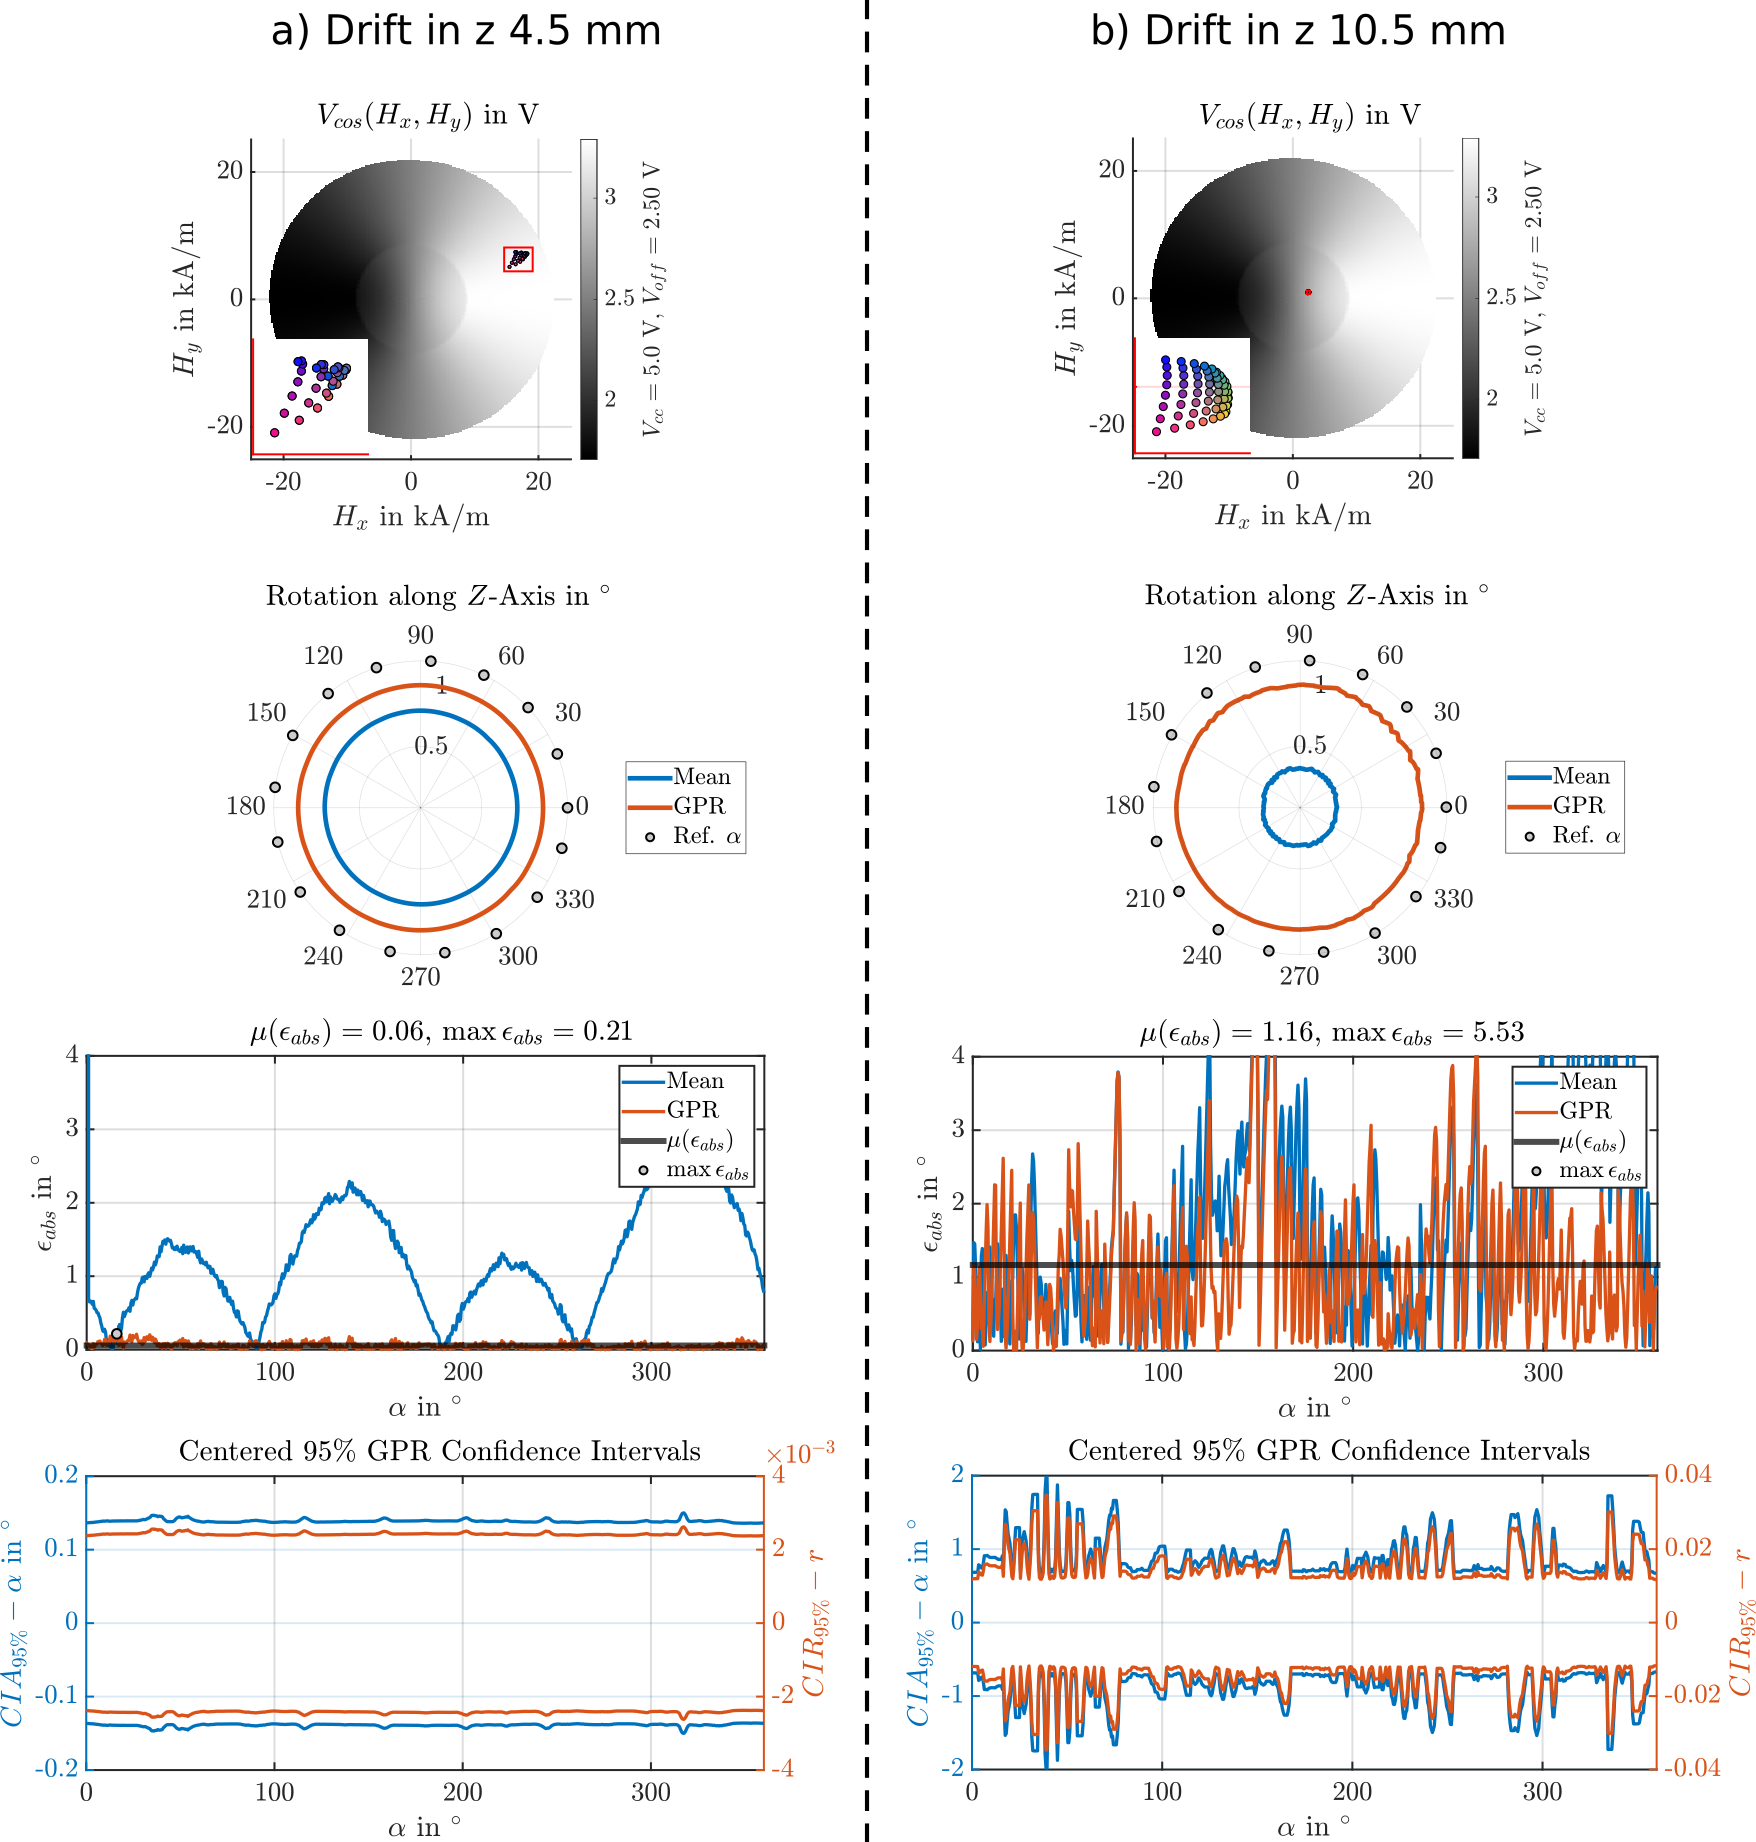
\includegraphics[width=\linewidth]{appendix/images/8-Ergebnisse-Experimente/Z-Pos-Comp-45-105-Rotation}
	\caption[Zpos 45 105 comp rotation]{Zpos a) 45 b) 105 comp rotation $\SI{21,5}{\degree}$ comp char spredding}
	\label{fig:z-pos-comp-45-105-rotation}
\end{figure}



\clearpage


\section{Verhalten bei kombinierten Fehllagen}\label{sec:ergexp6}

\begin{figure}[tbph]
	\centering
	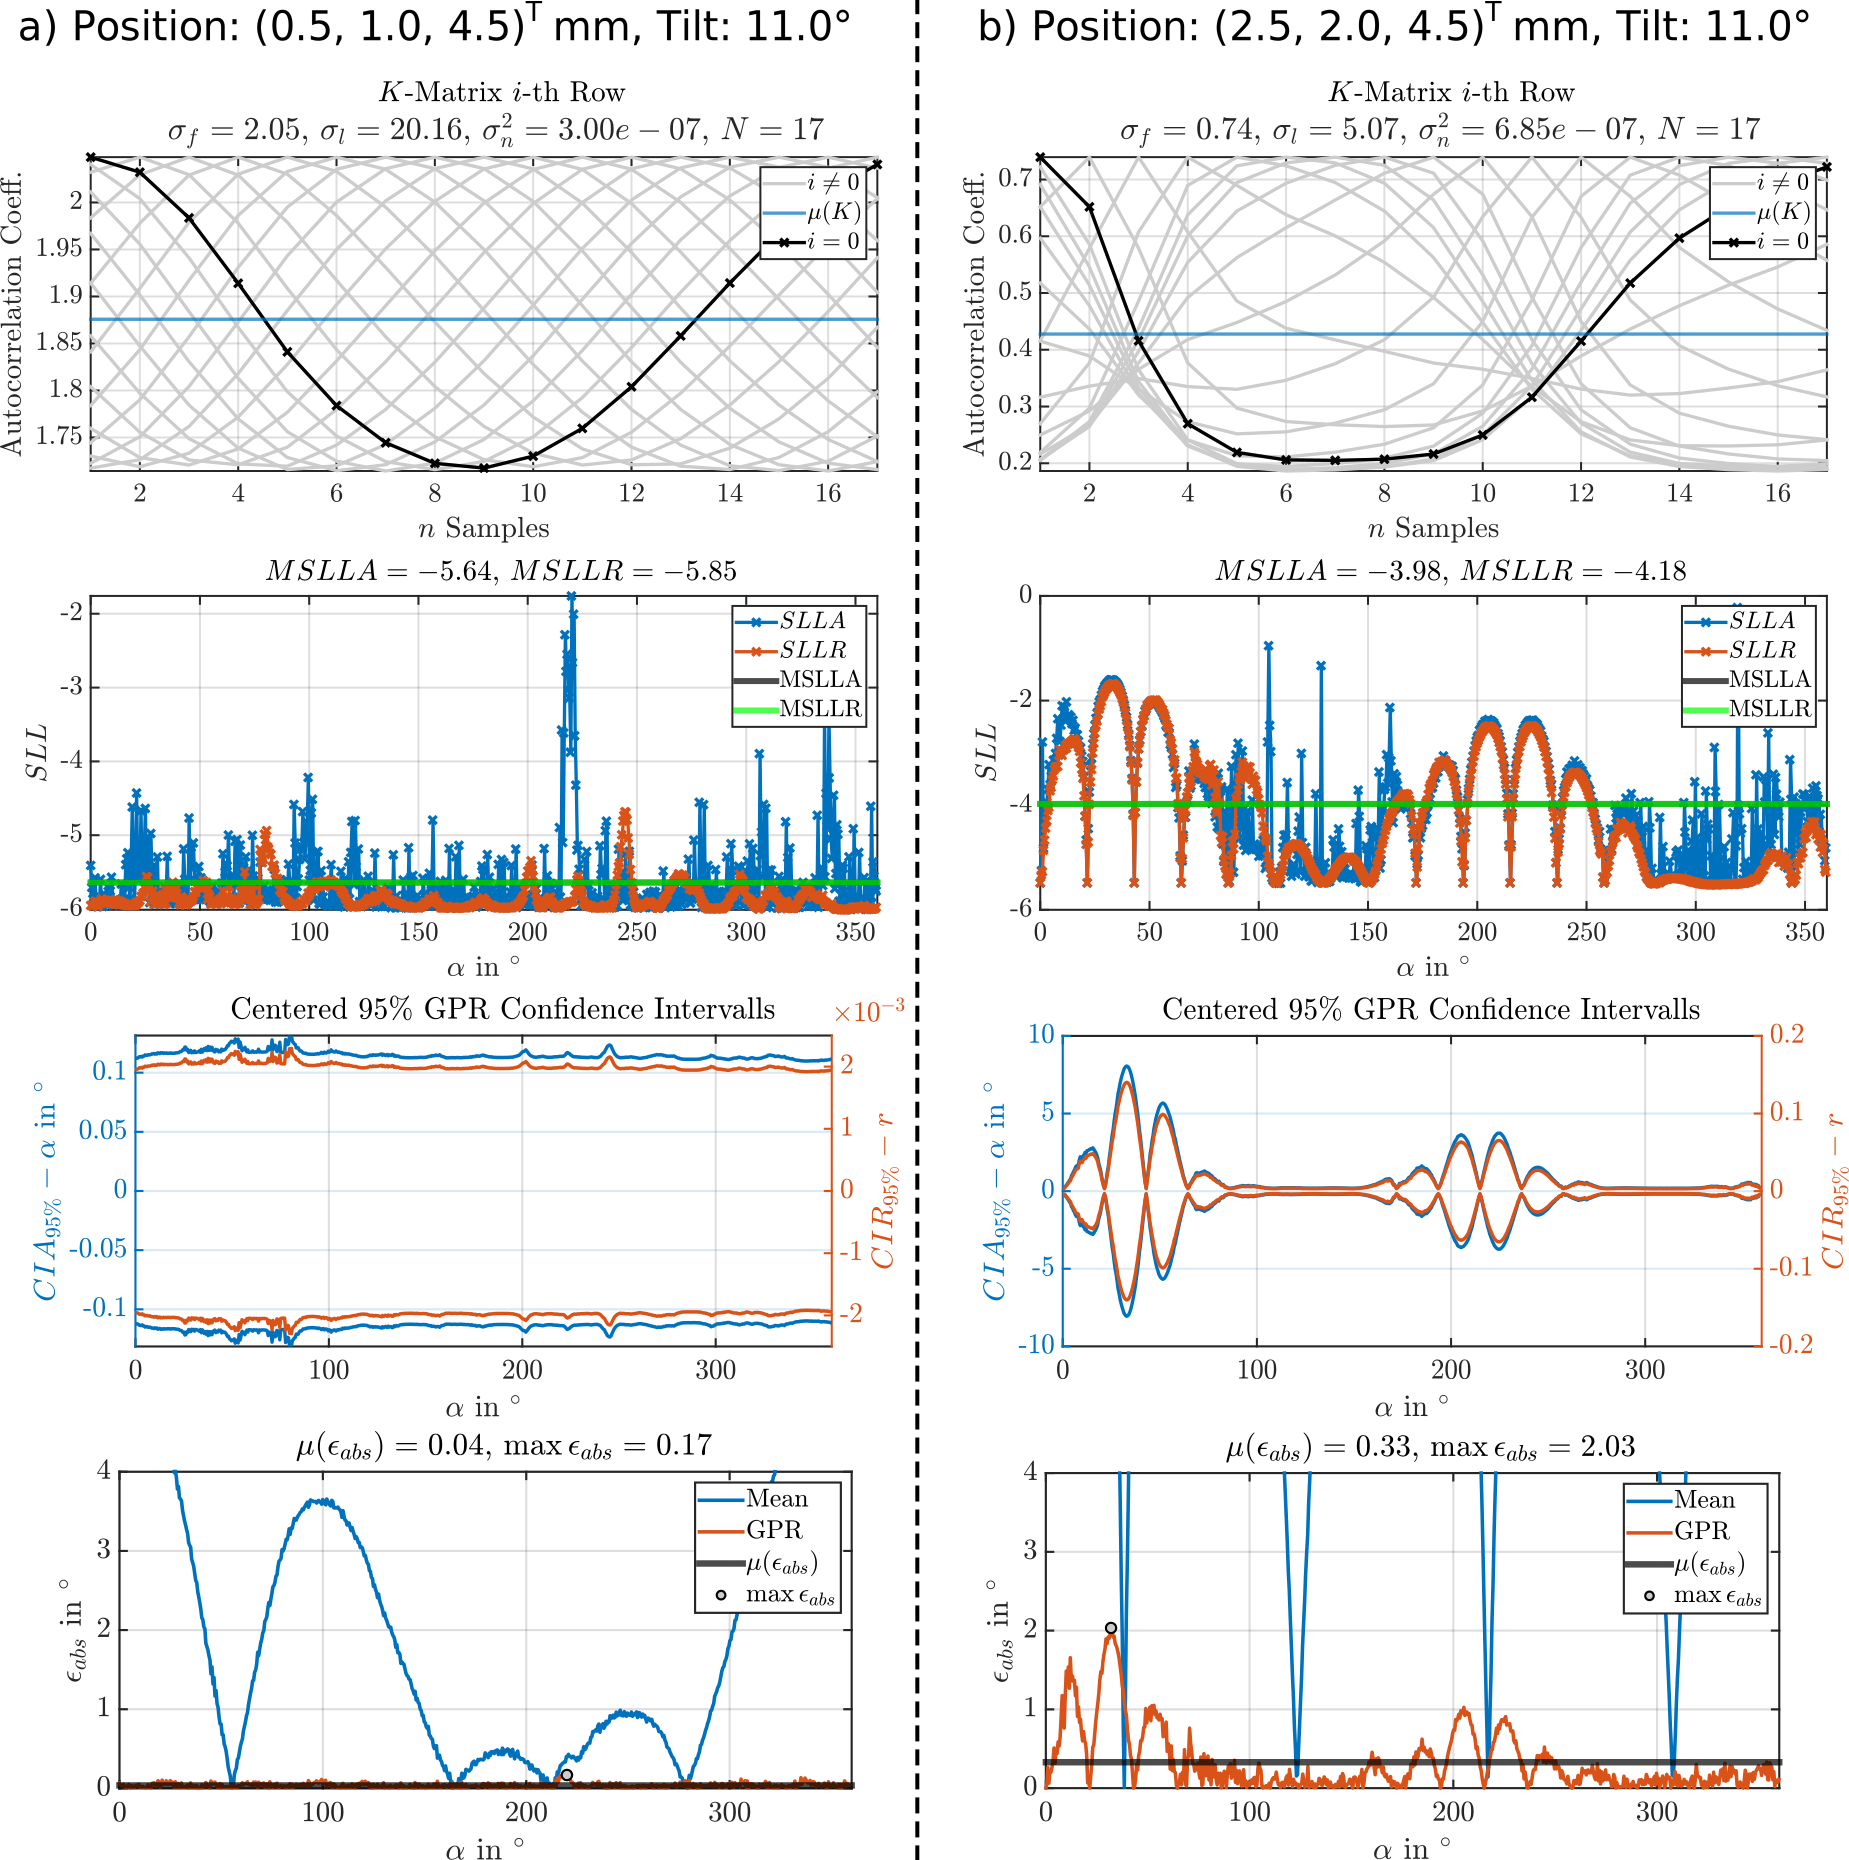
\includegraphics[width=\linewidth]{appendix/images/8-Ergebnisse-Experimente/Kombinierte-Fehllagen-GPR}
	\caption[Kombinierte Fehllagen Modell]{Kombinierte Fehllagen Modell}
	\label{fig:kombinierte-fehllagen-gpr}
\end{figure}



\begin{figure}[tbph]
	\centering
	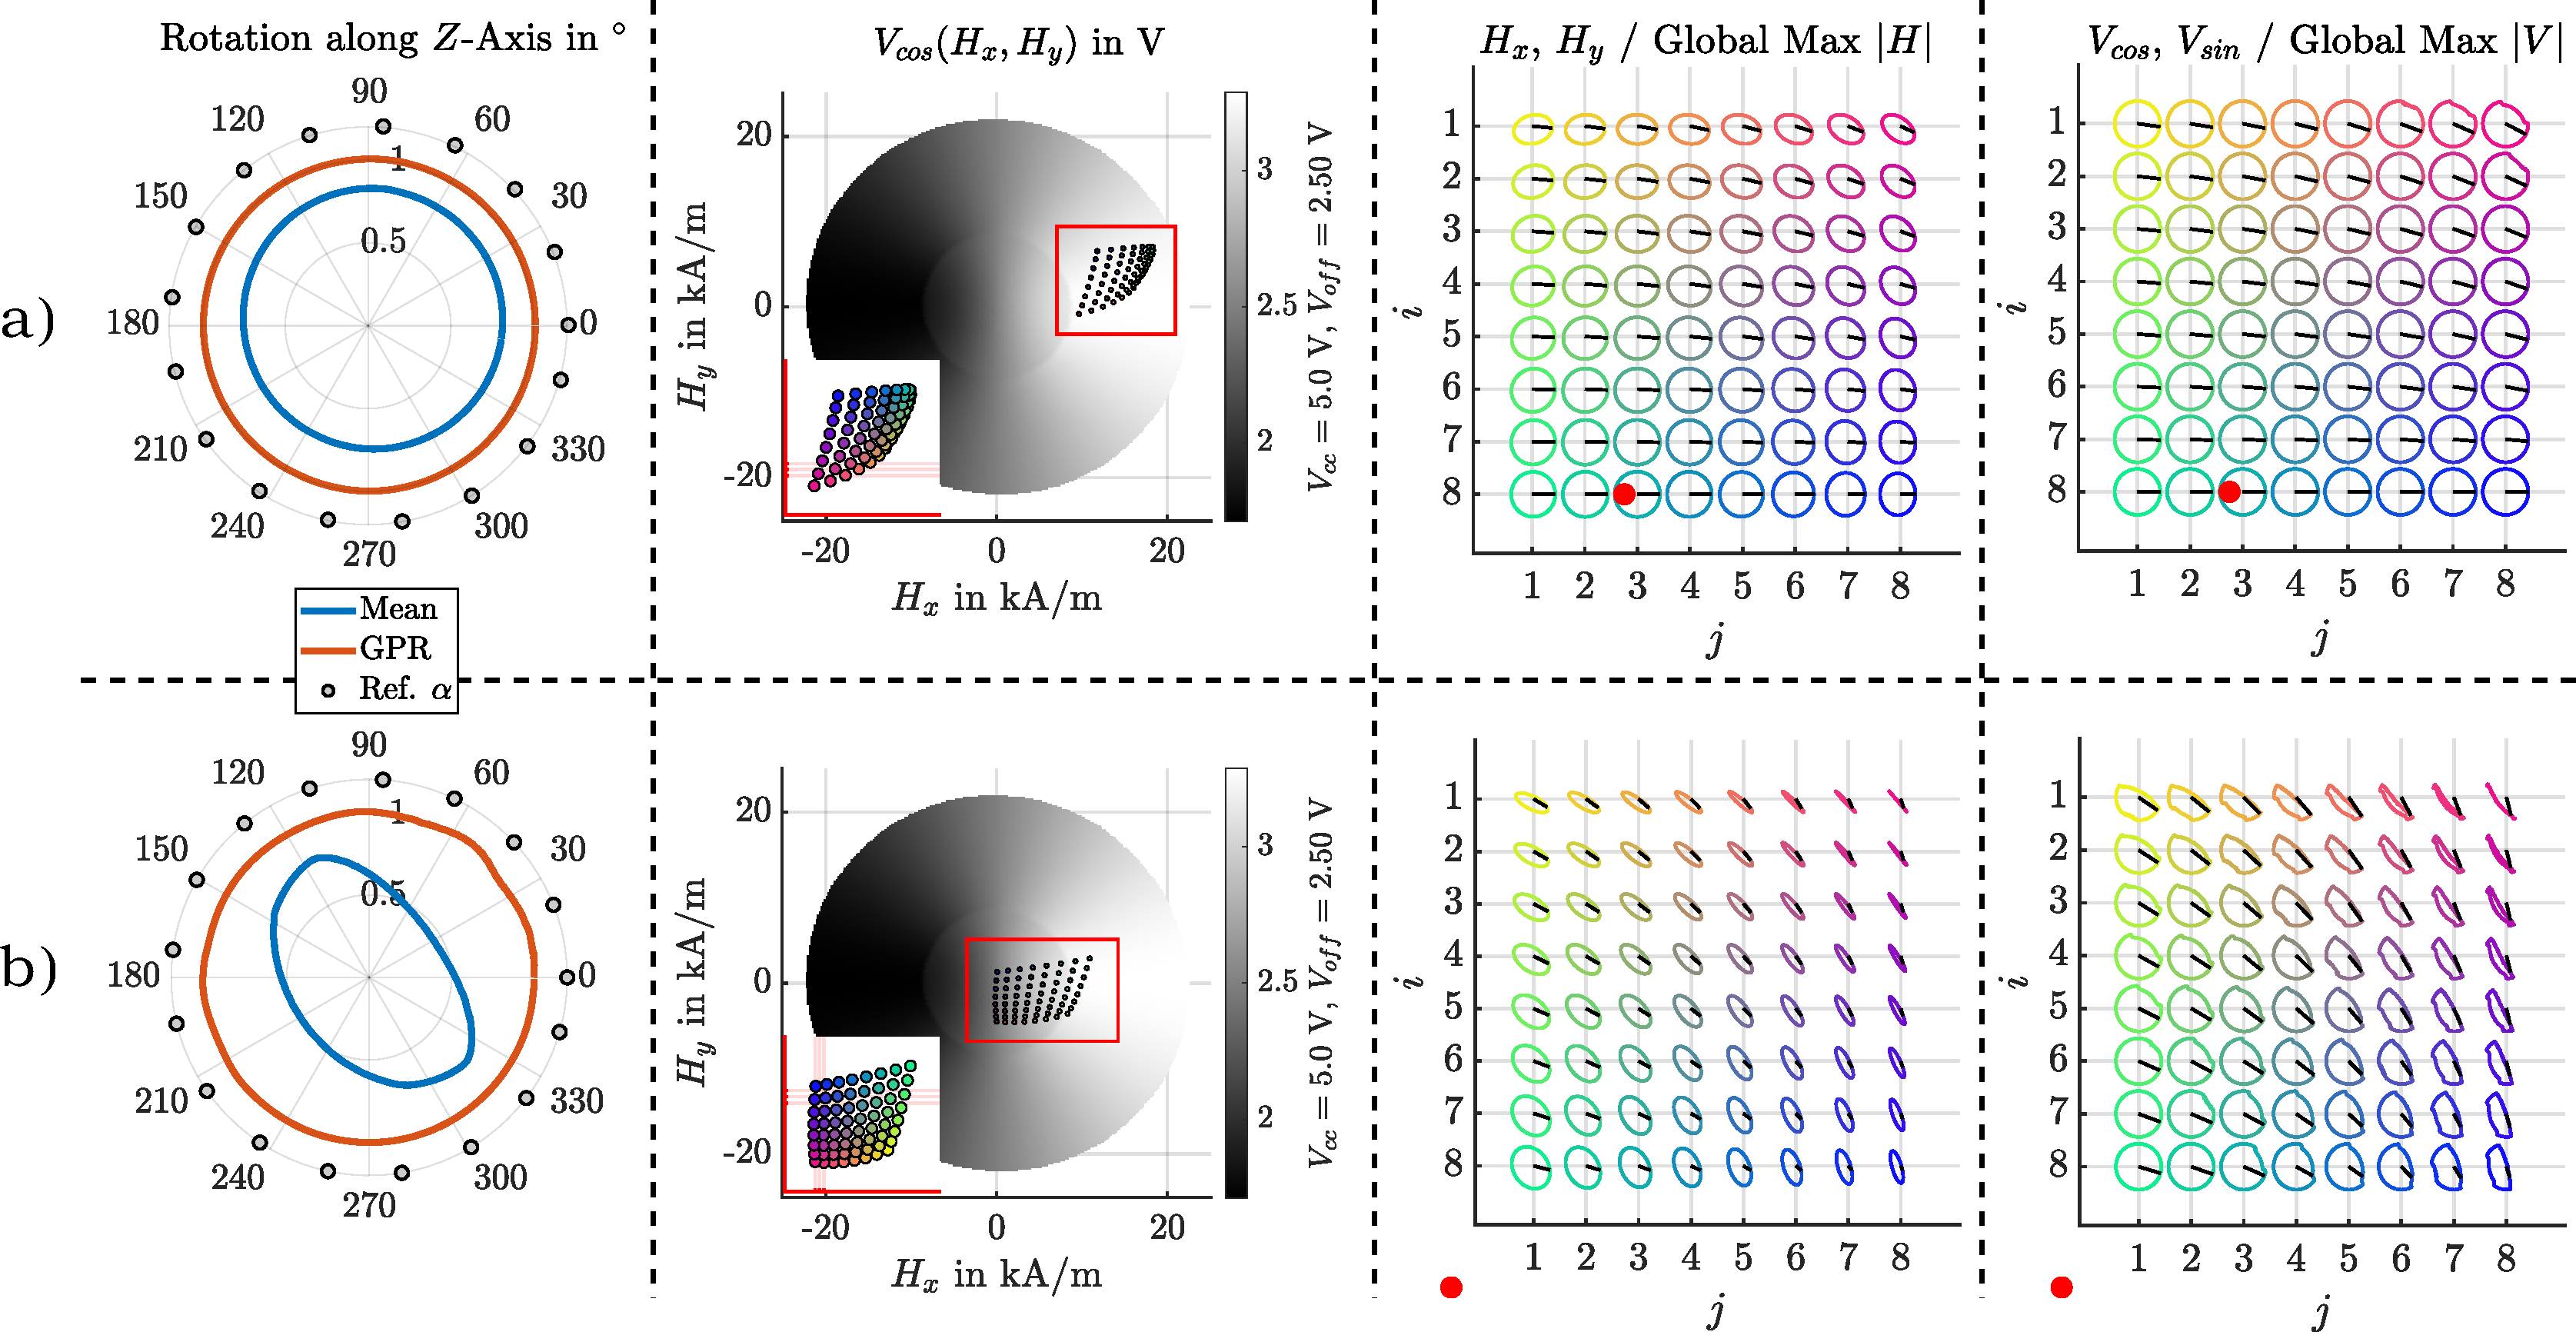
\includegraphics[width=\linewidth]{appendix/images/8-Ergebnisse-Experimente/Kombinierte-Fehllagen-Sensor}
	\caption[Kombinierte Fehlagen Sensor]{Kombinierte Fehlagen Sensor beide 11 tilt a) (0,0,4.5) b) (2.5,2,4.5) Verzerrung}
	\label{fig:kombinierte-fehllagen-sensor}
\end{figure}



%% !TEX root = ../thesis.tex
% appendix NXP KMZ60 char dataset
% @author Tobias Wulf
%

\chapter{NXP KMZ60 Kennfelddatensatz 0.0.1 29.03.2021}\label{ch:kmz60-datensatz}


\begin{figure}[tbph]
	\centering
	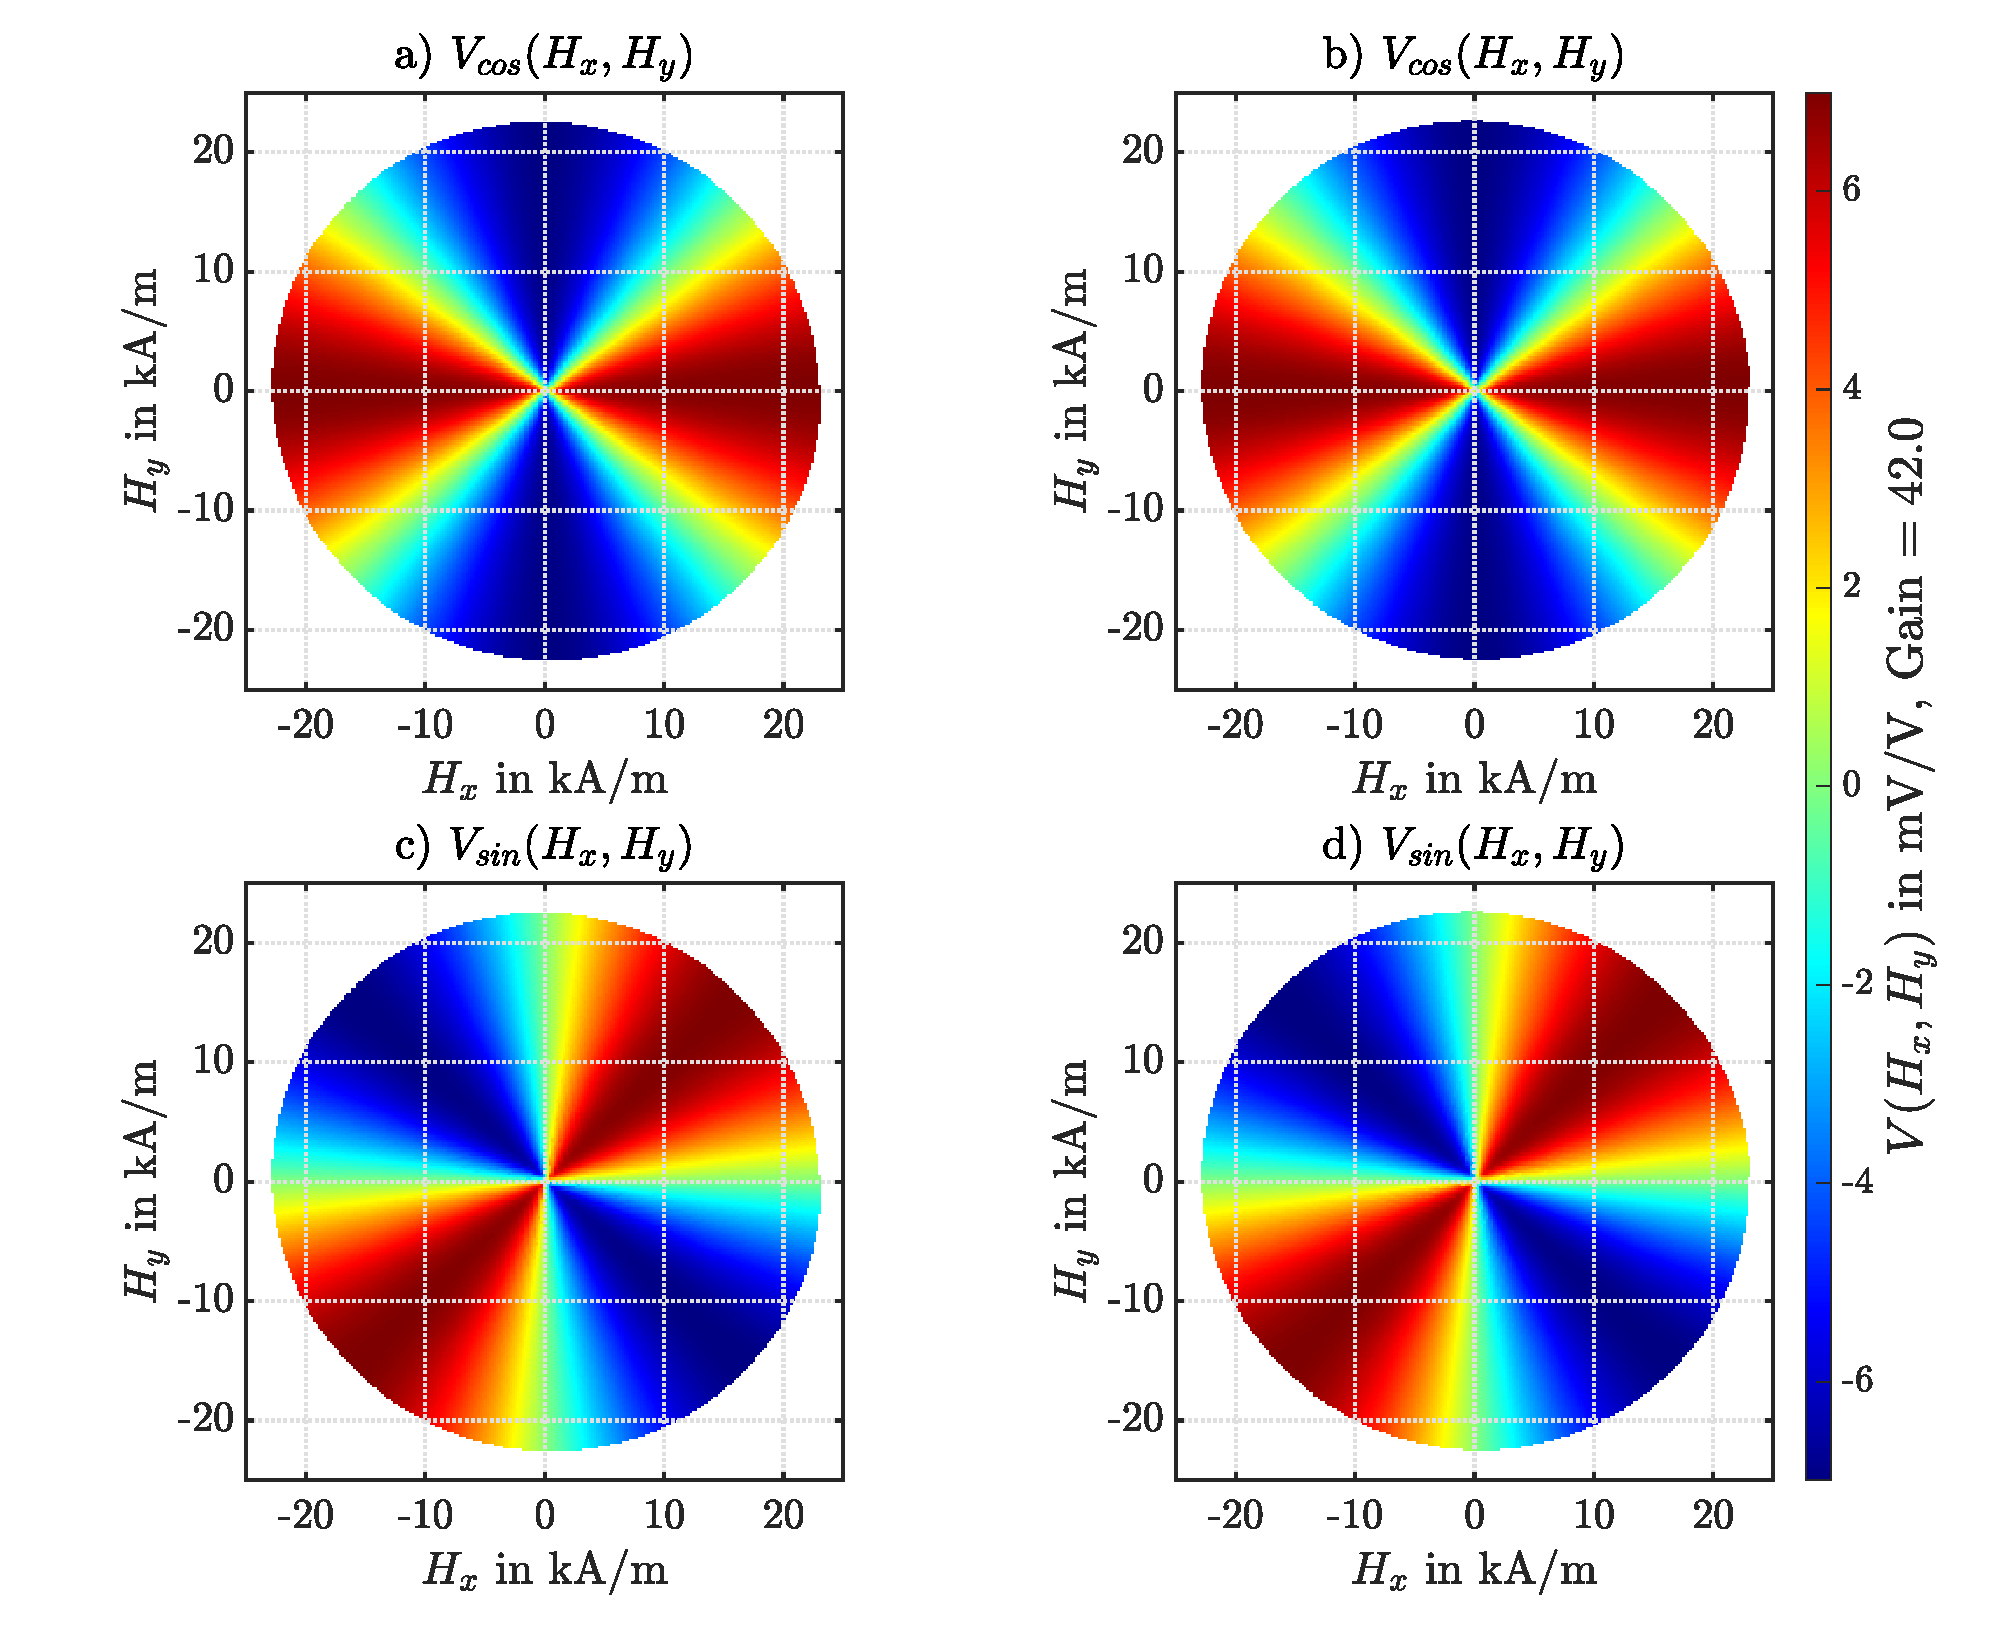
\includegraphics[width=\linewidth]{appendix/images/4-KMZ60/KMZ60_Kennfelder}
	\caption[NXP KMZ60 Winkelsensorbrückenkennfelder]{NXP KMZ60 Winkelsensorbrückenkennfelder. Zu sehen sind die 
		Kennfelder der Cosinus-Brücke a) und b). Darunter befinden sich die Kennfelder der Sinus-Brücke c) und d). 
		Die Kennfelder für beide Brücken a) und c) beziehen sich auf die steigenden Flanke der Amplitudenmodulation aus 
		\autoref{fig:magnetfeldstimuluskennfeldmethode} und die in b) bzw. d) gezeigten Kennfelder sind gewonnen aus 
		der fallenden Flanke. Die Brückenkennfelder sind normiert in $\SI{}{\milli\volt\per\volt}$. Für eine 
		Spannungsausgabe in Betriebsspannungsniveau ist eine zusätzliche Verstärkung um Faktor $42$ notwendig. Die 
		Kennfelder besitzen, jeweils in $H_x$- und $H_y$-Richtung, eine Schrittweite von 
		$\SI{0.1961}{\kilo\ampere\per\metre}$ und sind skaliert von $\SI{-25}{\kilo\ampere\per\metre}$ bis 
		$\SI{+25}{\kilo\ampere\per\metre}$. Somit ergibt sich eine Bildauflösung für ein Kennfeld von $256 \times 256$ 
		Messpunkten. Grafik nachempfunden aus \cite{Schuethe2019}.}
	\label{fig:kmz60kennfelder}
\end{figure}


\begin{figure}[tbph]
	\centering
	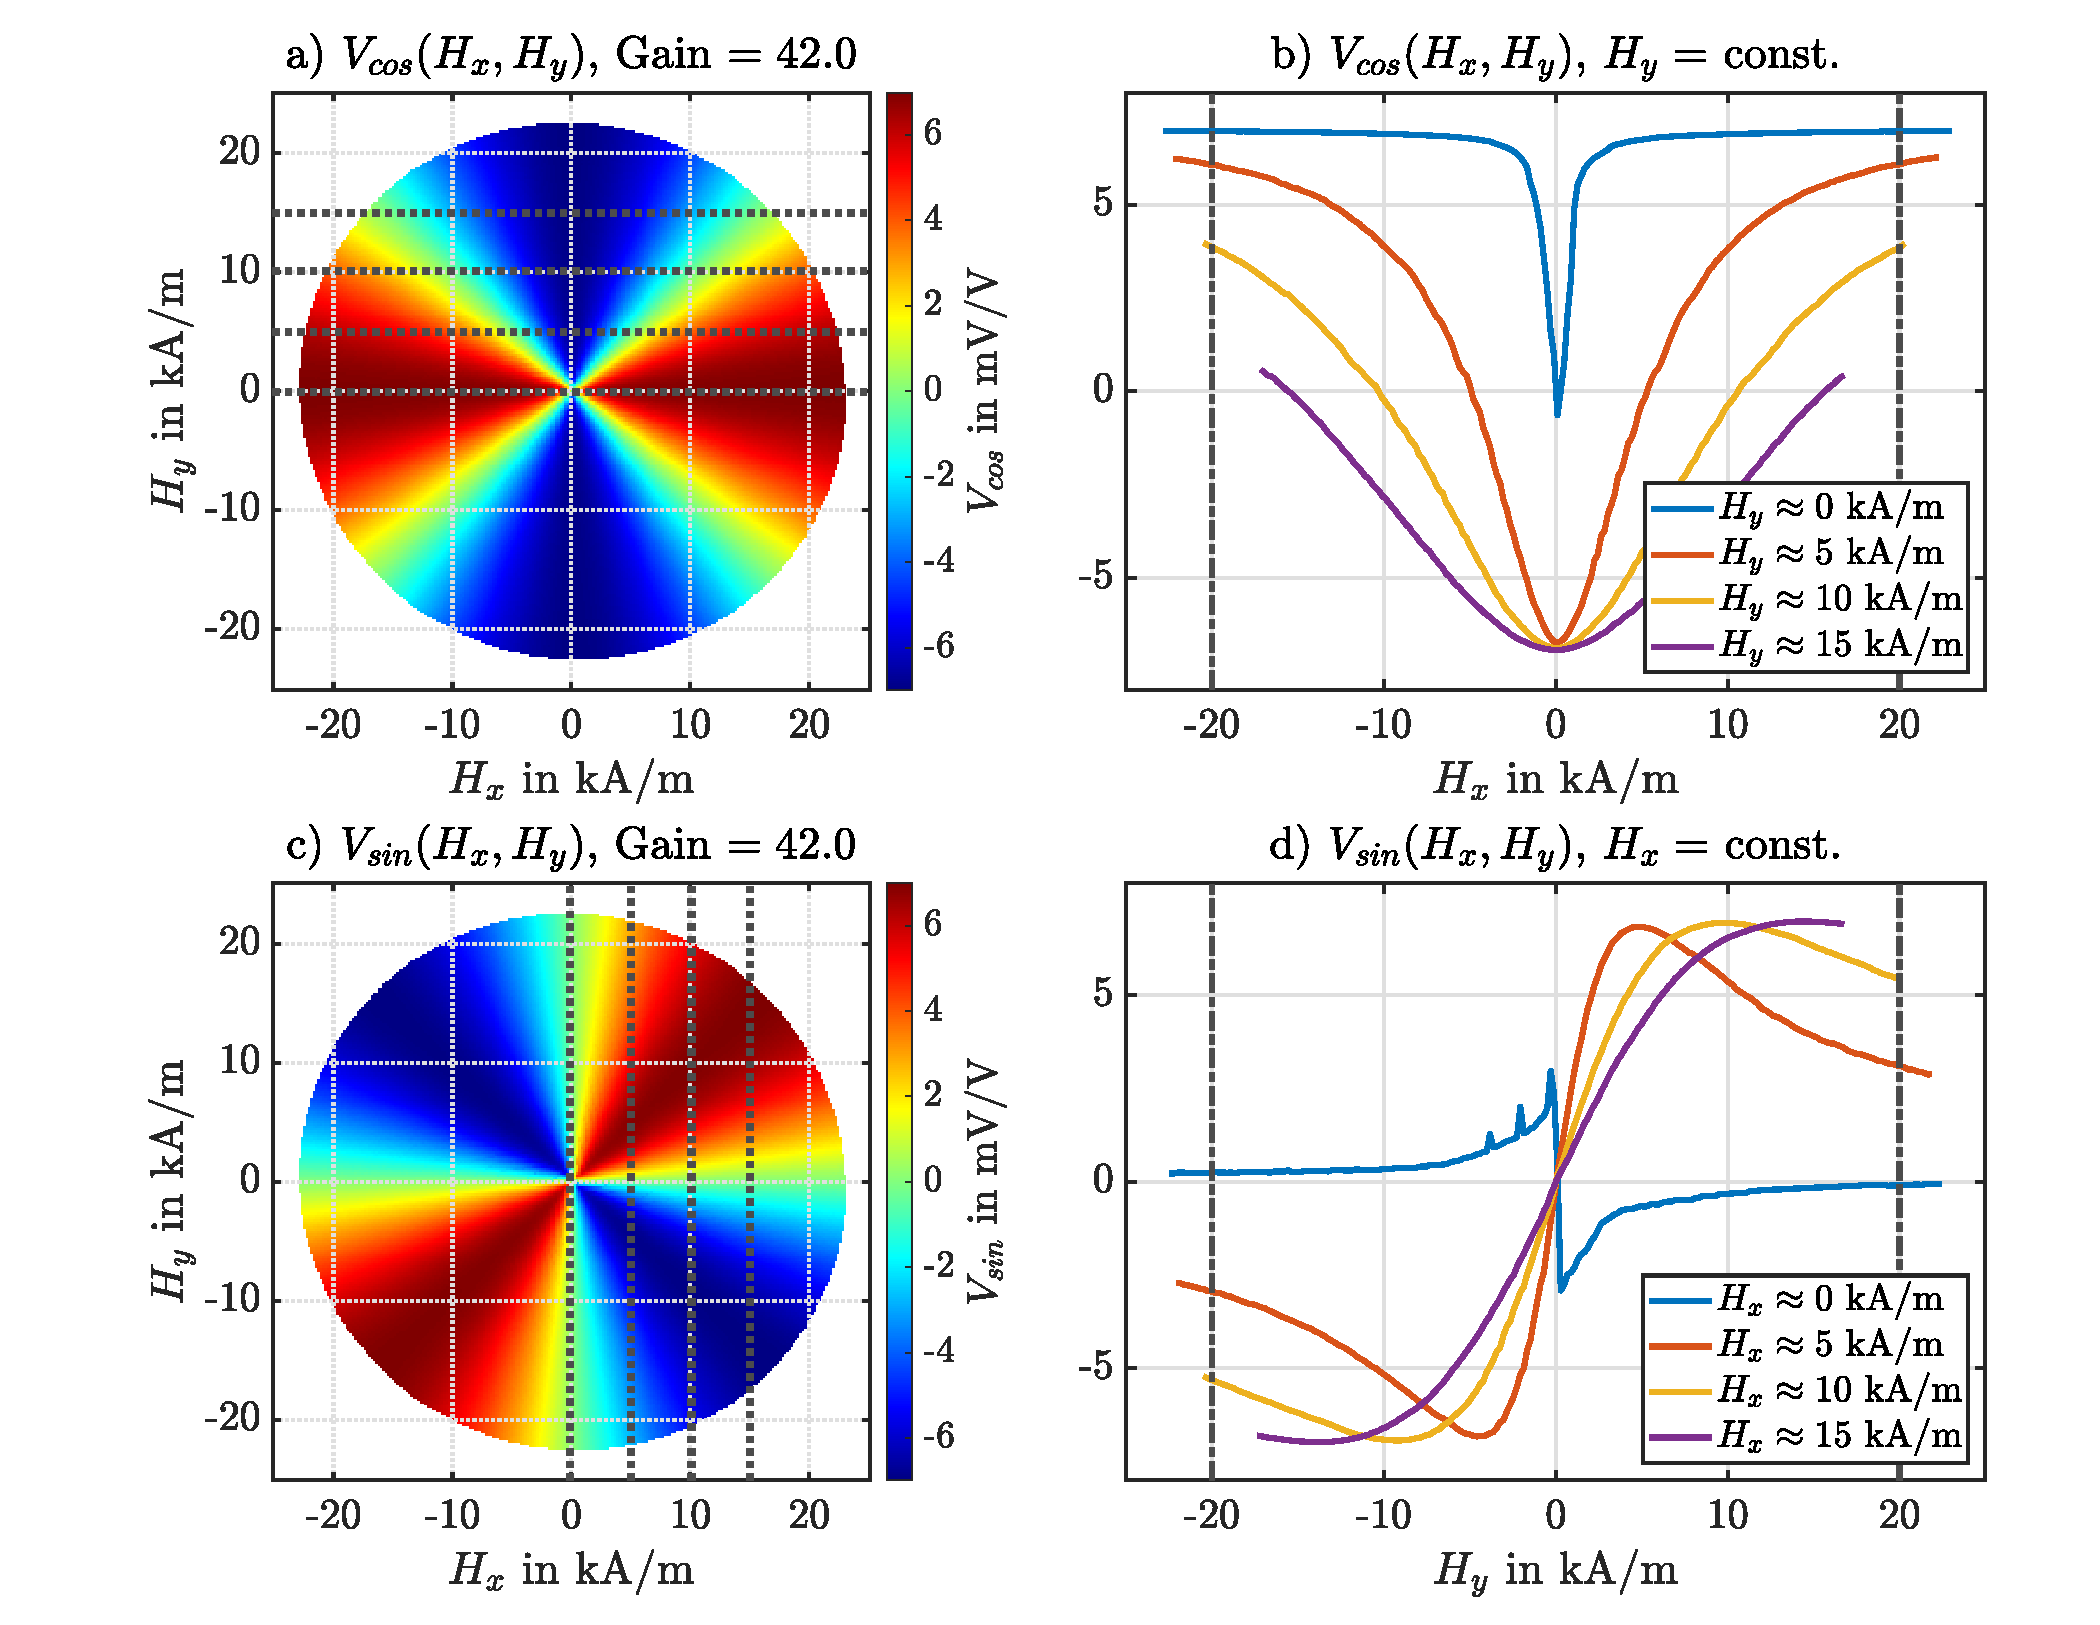
\includegraphics[width=\linewidth]{appendix/images/4-KMZ60/KMZ60_Kennfeld_Steigend}
	\caption[NXP KMZ60 Kennfeldquerschnitte]{NXP KMZ60 Kennfeldquerschnitte. Für die Kennfelder gewonnen aus 
		steigender Amplitudenmodulation a) und c). Es sind Querschnitte durch die jeweiligen Kennfelder in b) und d) 
		abgebildet. Für $V_{cos}$ a), b) verschiedene konstante $H_y$ und $V_{sin}$ c), d) entsprechend verschiedene 
		konstante $H_x$ Querschnitte. Grafik nachempfunden aus \cite{Schuethe2019}.}
	\label{fig:kmz60kennfeldsteigend}
\end{figure}




\begin{figure}[tbph]
	\centering
	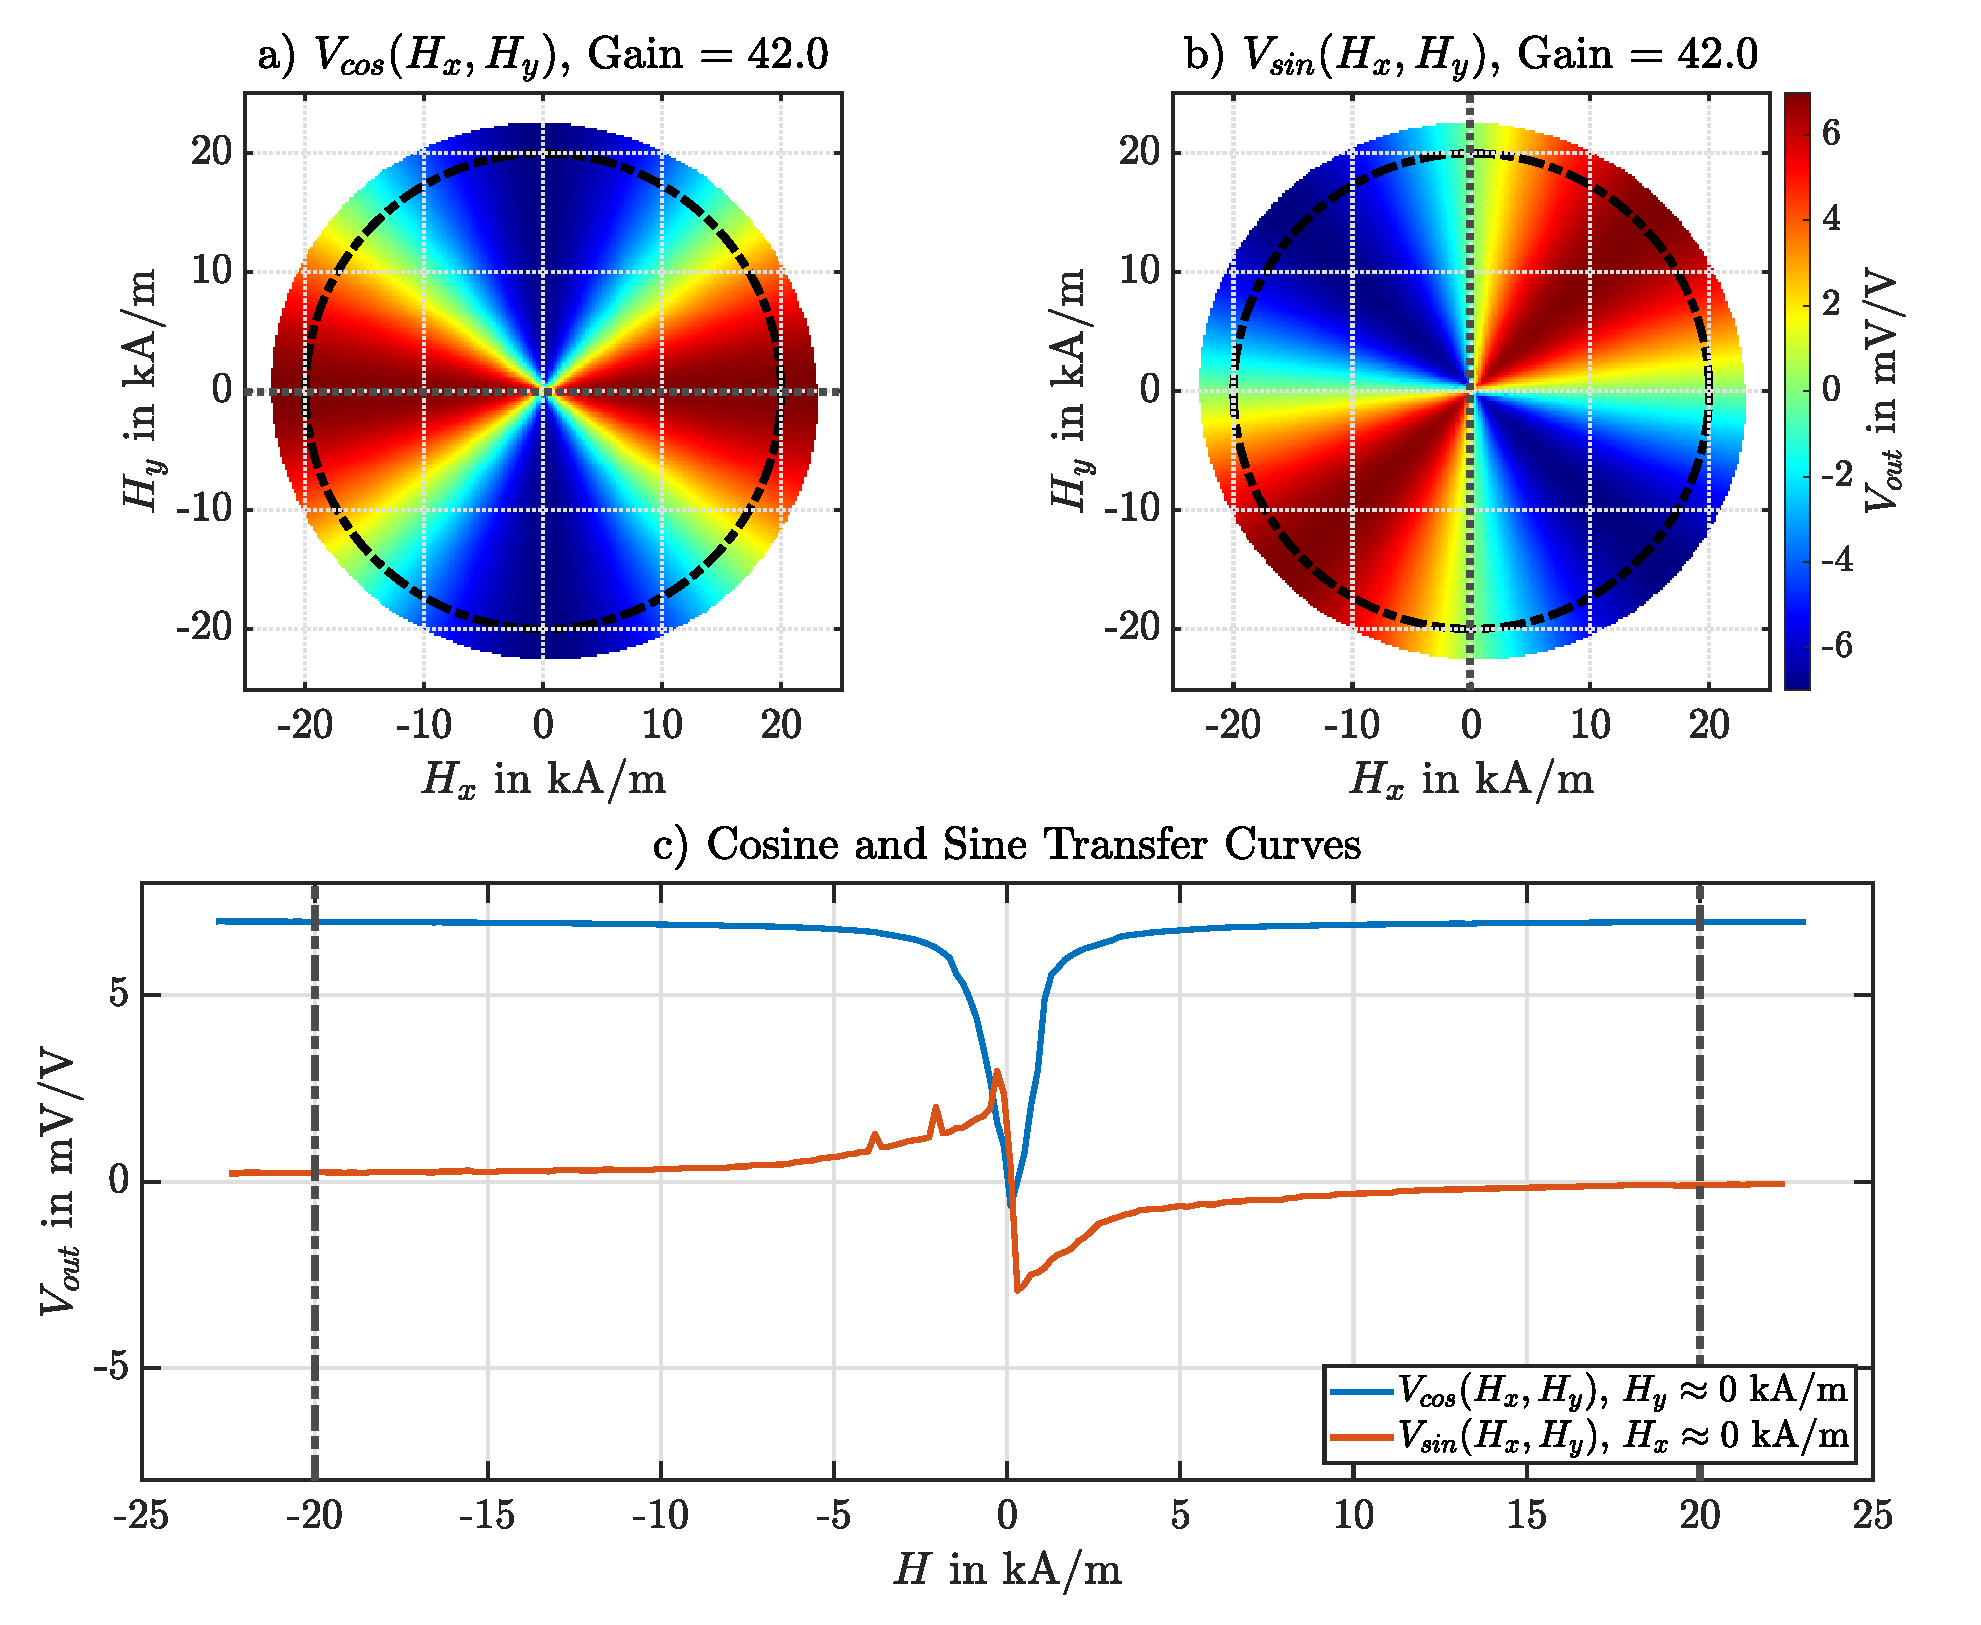
\includegraphics[width=\linewidth]{appendix/images/4-KMZ60/KMZ60_Uebertragungskennlinien}
	\caption[NXP KMZ60 Übertragungskennlinie]{NXP KMZ60 Übertragungskennlinie. Es sind wieder die Kennfelder aus 
		der steigenden Amplitudenmodulation in a) und b). In c) sind die Übertragungskennlinien für den Sensor gezeigt 
		mit Kennzeichnung für den Betrieb in Sättigung bei $\SI{20}{\kilo\ampere\per\metre}$. Ebenfalls zu sehen in a) 
		und b) durch die sich ergebene Kreisbahn mit einem Radius des aufgelegten Intervalls aus c). Grafik 
		nachempfunden aus \cite{Schuethe2019}.}
	\label{fig:kmz60uebertragungskennlinien}
\end{figure}

% !TEX root = ../thesis.tex
% appendix used software
% @author Tobias Wulf
%
\chapter{Genutzte Software 0.0.3 08.01.2021}\label{ch:genutzte-sw}

Für die Nachvollziehbarkeit der getätigten Entwicklungsarbeiten und die Erstellung der Bachelor-Thesis, ist das dafür jeweilige \gls{ac:os}
und die verwendete \gls{ac:sw} tabellarisch aufgeführt. Es finden sich genutzte Versionen der SW und Angaben zur Minimalanforderung für deren
Nutzung. Die Anforderungen sind für \gls{ac:cpu}, \gls{ac:ram}, \gls{ac:hdd} näher aufgeschlüsselt. Die Programmierarbeiten mit MATLAB sind
jeweils mit Windows und Linux geschrieben bzw. getestet worden.

\vspace{5mm}
\begin{table}[!htbp]
\centering
\resizebox{\textwidth}{!}{
\begin{tabular}{@{}lllll@{}}
\toprule
\textbf{Software}     & \textbf{Verwendungszweck (Typ)} & \textbf{Min.-Anforderung}    & \textbf{Version} & \textbf{Erscheinungstag} \\ \midrule
Ubunut Budgie         & Linux-Betriebssystem            & 2 GHz Dual-Core-CPU          & 18.04 LTS        & 26.04.2018               \\
                      & (Laptop OS)                     & 4 GB RAM                     &                  &                          \\
                      &                                 & 25 GB freier HDD-Speicher    &                  &                          \\ \hline
Windows 10 Enterprise & Windows-Betriebssystem          & 1 GHz Core-CPU               & 1909             & 12.11.2020               \\
                      & (Laptop OS)                     & 1 GB RAM                     &                  &                          \\
                      &                                 & 32 GB freier HDD-Speicher    &                  &                          \\ \hline
MATLAB                & Simulationssoftware             & Intel/ AMD x86-64 CPU        & 2020b            & 17.09.2020               \\
                      & (Multi-Paradigmen Programmier-  & 4 GB RAM                     &                  &                          \\
                      & Sprache, IDE)                   & 3.5 GB freier HDD-Speicher   &                  &                          \\ \hline
Git                   & Versionierung                   & -                            & 2.29             & 29.10.2020               \\
                      & (Kommandozeilenprogramm)        & -                            &                  &                          \\
                      &                                 & -                            &                  &                          \\ \hline
Inkscape              & Vektorgrafikzeichenprogramm     & 1 GHz CPU                    & 0.92.3           & 11.03.2018               \\
                      & (Grafikaufbereitung)            & 256 MB RAM                   &                  &                          \\
                      &                                 & 302 MB freier HDD-Speicher   &                  &                          \\ \hline
Texstudio             & Textbearbeitung f. LaTeX        & -                            & 2.12.6           & 25.07.2020               \\
                      & Dokumente (Editor)              & -                            &                  &                          \\ 
                      &                                 & 24.7 MB freier HDD Speicher  &                  &                          \\ \hline
wkhtmltopdf			  & HTML- zu Pdf-Konvertierung      & -                            & 0.12.6           & 11.06.2020               \\
                      &                                 & -                            &                  &                          \\
                      &                                 & -                            &                  &                          \\ \hline
JabRef				  &	Literaturverwaltungsprogramm    & -							   & 5.1              & 30.08.2020               \\
                      & f.BibLaTeX (Editor)             & -                            &                  &                          \\
                      &                                 & -                            &                  &                          \\
\bottomrule		
\end{tabular}}
\caption[Genutzte Software]{Genutzte Software zur Erstellung der Thesis und Dokumentation der Ergebnisse, Entwicklungsumgebung für die
geschriebene Simulationssoftware zur Generierung und Auswertung der Sensor-Array-Simulation.}
\label{tab:sw}
\end{table}

% !TEX root = ../thesis.tex
% appendix software documentation (autogenerated)
% @author Tobias Wulf
%
\chapter{Software-Dokumentation 0.0.4 13.01.2021}\label{ch:sw-doku}

Die Software-Dokumentation ist automatisiert mit MATLAB-Skripten erstellt worden.
Es ist dafür ein zweistufiger Prozess implementiert, der im ersten Schritt eine
in MATLAB integrierte HTML-Dokumentation erstellt und im Anschluss diese zu
eigenständigen PDF-Dateien exportiert. Als letzter Schritt sind diese zu einem LaTeX-Manual
zusammengefasst im Anhang eingebunden. Mit diesem Verfahren ist es möglich,
eine Dokumentation direkt aus geschriebenen M-Dateien zu generieren. Allerdings
ist es dafür nötig, eine spezielle Formatierung und einen gewissen Programmierstil einzuhalten \cite{Johnson2014}.
Die Dokumentation enthält neben dem erstellten Quellcode eine Reihe von Arbeitsanweisungen,
wie mit der Software umzugehen ist. Zusätzlich sind Beschreibungen für die Erstellung und Pflege
des Software-Projektes mit beigefügt. Die geschriebene Software ist mithilfe
des Software-Versionierungsprogramms Git erstellt worden, was eine genaue Nachvollziehbarkeit in Bezug
auf die einzelnen Arbeitsschritte ermöglicht. Zur Versionierung ist der Git-Feature-Branch-Workflow \cite{Bitbucket2020}
angewandt worden. Aus stilistischen Gründen ist die gesamte Software-Dokumentation in Englisch verfasst.

% \subimport{../../Manual/}{Manual.tex}



\Istatement

\end{document}
